\documentclass{report}

\usepackage[dvipsnames,x11names]{xcolor}
\usepackage[utf8]{inputenc}
\usepackage[T1]{fontenc}
\usepackage[british]{babel}
\usepackage{etoolbox}
\newbool{isRelease}
\IfFileExists{.isRelease}{\booltrue{isRelease}}{\boolfalse{isRelease}}
\usepackage[margin=2.5cm]{geometry}
\usepackage{amssymb, latexsym, mathtools}
\usepackage{times}
\usepackage{float}
\usepackage{listings}
\usepackage{natbib}
\usepackage{framed}
\ifbool{isRelease}
    {\usepackage[disable]{todonotes}}
    {\usepackage{todonotes}}

\usepackage{amsmath}
\usepackage{stmaryrd}
\usepackage{colonequals}

\usepackage{tikz}
\usetikzlibrary{automata, positioning, arrows}
\tikzset{
    state/.style={
           rectangle,
           rounded corners,
           draw=black, very thick,
           minimum height=2em,
           inner sep=2pt,
           text centered,
           },
}


\usepackage{microtype}
\usepackage{graphicx}

\usepackage[colorlinks,citecolor=blue,linkcolor=blue,anchorcolor=blue,urlcolor=blue]{hyperref}
\usepackage[capitalise,noabbrev,nameinlink]{cleveref}

\usetikzlibrary{arrows}

\newcommand{\coot}[1]{\textcolor{violet}{\emph{#1}}}
\newcommand{\njd}[1]{\textcolor{purple}{\emph{#1}}}
\newcommand{\avieth}[1]{\textcolor{blue}{\emph{#1}}}
\newcommand{\dcoutts}[1]{\textcolor{orange}{\emph{#1}}}
\addtolength{\marginparwidth}{-0.1\marginparwidth}

\newcommand{\var}[1]{\mathit{#1}}
\newcommand{\type}[1]{\mathsf{#1}}
\newcommand{\powerset}[1]{\mathbb{P}(#1)}
\newcommand{\order}[1]{\mathcal{O}\left(#1\right)}
\newcommand{\restrictdom}{\lhd}
\newcommand{\subtractdom}{\mathbin{\slashed{\restrictdom}}}
\newcommand{\restrictrange}{\rhd}

\ifbool{isRelease}
       {
         \newcommand{\wip}[1]{}
         \newcommand{\hide}[1]{}
       }
       {
         \newcommand{\wip}[1]{\color{magenta}{#1}\color{black}}
         \newcommand{\hide}[1]{}
       }
\newcommand{\haddockref}[2]
           {\href{https://input-output-hk.github.io/ouroboros-network/#2}
                 {\emph{haddock documentation}: \texttt{#1}}
           }
\newcommand{\trans}[1]{\texttt{#1}}
\newcommand{\state}[1]{\texttt{#1}}
\newcommand{\msg}[1]{\texttt{#1}}
\newcommand{\StIdle}{\state{StIdle}}
\newcommand{\StBusy}{\state{StBusy}}
\newcommand{\StDone}{\state{StDone}}
\newcommand{\MsgDone}{\msg{MsgDone}}

% TODO: the document is using `\langle` and `\rangle` to denote lists, maybe
% it's better to use Haskell notation, will it be more in sync with other docs
% produced by the formal method team?
\renewcommand{\langle}{[}
\renewcommand{\rangle}{]}

\DeclareMathOperator{\dom}{dom}
\DeclareMathOperator{\range}{range}
\DeclareMathOperator*{\argmin}{arg\,min} % thin space, limits underneath in displays
\DeclareMathOperator*{\minimum}{min}
\DeclareMathOperator*{\maximum}{max}

% ---- Connection Manager things
\lstset{
  xleftmargin=2pt,
  stepnumber=1,
  belowcaptionskip=\bigskipamount,
  captionpos=b,
  escapeinside={*'}{'*},
  language=haskell,
  tabsize=2,
  emphstyle={\bf},
  commentstyle=\it,
  stringstyle=\mdseries\rmfamily,
  showspaces=false,
  keywordstyle=\bfseries\rmfamily,
  columns=flexible,
  basicstyle=\small\sffamily,
  showstringspaces=false,
  morecomment=[l]\%,
}
\lstdefinelanguage{cddl}{
  morekeywords={bool,uint,nint,int,float16,float32,float64,float,bstr,bytes,tstr,text},
  morecomment=[l]{;},
  morestring=[b]",
}
\lstdefinestyle{cddl}{
  numbers=left,
  language=cddl,
  columns=fixed,
}

\definecolor{shadecolor}{rgb}{.6,0.6,0.8}
\definecolor{mygreen}{rgb}{0.109804,0.698039,0.341176}
\definecolor{myblue}{rgb}{0.360784,0.423529,255}
\usetikzlibrary{arrows,calc,matrix,shapes}
\tikzset{every scope/.style={>=triangle 60,thick}}
\exhyphenpenalty 10000

% -------

\raggedbottom

\begin{document}

\title{The Shelley Networking Protocol}
\author{
  Duncan Coutts \\
  {\small \texttt{duncan@well-typed.com}} \\
  {\small \texttt{duncan.coutts@iohk.io}}
\and
  Neil Davies \\
  {\small \texttt{neil.davies@pnsol.com}} \\
  {\small \texttt{neil.davies@iohk.io}}
\and
  Karl Knutsson \\
  {\small \texttt{karl.knutsson@iohk.io}}
\and
  Marc Fontaine \\
  {\small \texttt{marc.fontaine@iohk.io}}
\and
  Armando Santos \\
  {\small \texttt{armando@well-typed.com}}
\and
  Marcin Szamotulski \\
  {\small \texttt{marcin.szamotulski@iohk.io}}
\and
  Alex Vieth \\
  {\small \texttt{alex@well-typed.com}}
}
\date{{\small Version 1.3.0, \today}}

\maketitle

\begin{abstract}
  This document provides technical specification of the implementation of the
  \texttt{ouroboros-network} component of \texttt{cardano-node}. It provides specification of all
  mini-protocols as well multiplexing and low level wire encoding.  It provides
  necessary information about both node-to-node and node-to-client protocols.

  The primary audience for this document are engineers wishing to build
  clients interacting with a node via node-to-client or node-to-node protocols
  or independent implementations of a node.  Although the original
  implementation of \texttt{ouroboros-network} is done \texttt{Haskell}, this specification is
  made language agnostic. We may provide some implementation details which are
  \texttt{Haskell} specific.
\end{abstract}

\tableofcontents

\section*{Version history}

\begin{description}
\item[Version 1.0.0 Nov 2019, State machines and wire format for Ouroboros-Network-1.0.0.]
\item[Version 1.1.0 Apr 2021, Connection Manager for Ouroboros-Network-Framework.]
\item[Version 1.2.0 Apr 2021, tx-submission version 2, local-state-query, keep-alive mini-protocols]
\item[Version 1.3.0 Jul 2021, Review of the multiplexer documentation]
\end{description}
% \chapter{Overview}
The Cardano blockchain system is based on the Ouroboros family of protocols
for a proof-of-stake cryptocurrency.
The operation of these protocols on a node, working in collaboration with the consensus
and ledger aspects of Cardano, create the overall distributed system.
It is that distributed system that defines the "single source of truth" that is the distributed ledger.
The Ouroboros papers describe these protocols in a high-level mathematical formalism
that allows for a concise presentation and is appropriate for peer review by cryptography experts.
For separation of concerns, the papers do not describe a concrete implementation of the Ouroboros
protocols.

This document has a broader scope.
It is addressed to system designers and engineers who have an IT background
but are not necessarily crypto experts,
but want to implement Cardano or to understand the reference implementation.
The description of the protocol in this document contains all the information needed to
implement the data diffusion functionality of a compatible Cardano network node.
It covers:
\begin{itemize}
\item How nodes join the network.
\item The general semantics of the messages that nodes exchange.
\item The binary format of the messages.
\item The order in which nodes send and receive the messages of the protocol.
\item The permissible protocol states for each participant in the protocol.
\end{itemize}
This information is typically found in the description of network protocols.

However, the Ouroboros proof-of-stake cryptocurrency has additional requirements,
of a sort that are not typically covered in a
protocol  description itself.
While these underlying requirements are essential for understanding the design of the protocol,
it also makes sense to also discuss these aspects and requirements in this document.
Typical network protocols describe simple information exchanges;
the distributed nature of blockchain computation means
that additional contextual information is available.
Use of this context allows, for example, for validated store and forward
which is an essential feature to contain the effect of potential malicious actions
against the distributed system.

Shelley is a first fully decentralised release of Cardano system, implementing the Ouroboros protocol.

This Chapter contains an overview of the content and scope of this document and aspects that
are being discussed.

\wip{
\subsubsection{Software assurance}
Software assurance
}

\subsubsection{Layered Protocols}
Traditionally network protocols are presented as a stack of layers where
upper layers build on services provided by lower layers and lower layers
are independent of the implementation of the upper layers.
This concept of layers is misleading when discussing Ouroboros.
For example, it is {\em not} the case that the consensus (layer)
is built on top of the network (layer).
It is more appropriate to talk about a network component than a network layer.
The network component provides services to the consensus component and vice versa;
both components rely on each other.
The network component uses the consensus component to validate
information that it distributes to other nodes, which
is essential to guard against certain kinds of DoS attacks.
Existing peer-to-peer systems focus on a slightly different problem domain.
For example, they do not consider the information validation issue
or are concerned with issues such as 'eclipse attacks' that to not
apply to the Ouroboros family of protocols.

%\missingfigure[figwidth=6cm]{Testing a long text string}

\subsubsection{Performance of the Ouroboros Network}
In computer science, Byzantine Fault Tolerance is a property of a distributed algorithm, which states
that it works for the honest participants
under the assumption that a certain proportion of the participants are indeed honest.
A similar, but more informal property applies to performance of the Ouroboros network as well.

The network provides a service to its participants while at the same
time the participants provide a service to the network.
The performance of the Ouroboros network depends (among other things) on the performance of the nodes,
while the performance of a node also depends on the performance of the network.
Not only are there honest and adversarial participant, but there is also a huge variety of
possible network topographies, bandwidths and latencies of network connections and other
factors that determine the performance of the network.

This document discusses the high level functional and performance requirements for Ouroboros and the
assumptions made about the structure of the underlying P2P network.

\subsubsection{Protocol vs Implementation}
Network Protocols are written at different levels of abstraction.
To be useful, a protocol description must be precise enough to be implemented.
A protocol description should also be abstract enough to allow alternative implementations of the protocol
and to facilitate developing and improving it.
Furthermore, it should be possible to both implement an
abstract version of a protocol
and interpret it in a real-world scenario.
For example, it must be possible to implement a protocol
such that the real-world software runs on a machine with a typical size of memory
and a typical speed network connection.

The Shelley network protocol design has been developed in parallel
with a reference implementation in Haskell.
Haskell (more precisely GHC) has built-in support for high level concurrency abstractions
such as light-weight threads and software transactional memory.
While the protocol itself is completely language agnostic, it still makes sense to discuss some
aspects of the Haskell reference implementation in this document.
In particular, the document describes how to achieve good resource bounds for
a protocol implementation.

\wip{
  \subparagraph{Threats}
  Reference the Threats section.
  'eclipse' can be deterred}


\wip{TODO:extended abstract, scope of the document}

\section{High level requirements and User Stories}

These are the high level business requirements for the networking that were
gathered and signed off in late 2017. As such they are expressed in informal
prose, often following a ``user story'' style.
Roughly, there are three different kinds of users:
\begin{itemize}
\item Users who have delegated.
\item Small stakeholders.
\item Large stakeholders.
\end{itemize}

\subsubsection{Network connectivity}\label{network-connectivity}

\paragraph{Participate as a user who has delegated}

As a Daedalus home user with my stake delegated to other users
I would like to join the Cardano network so I can participate in the network.
\begin{itemize}
\item The system must be designed to provide this user segment with the ability
      to catch up and keep up with the blockchain without having
      to do any local network configuration.
\item The system must be designed to provide this user segment with the ability to
      continuously find and maintain a discovery of a sufficient number of
      other network participants that have reasonable connectivity.
\item The system must be designed to provide this user segment with the ability to
      find and maintain a minimum of 3 other network participants to maintain
      connectivity with performance that is sufficient to catch up with the
      blockchain.
\item The system design will take into account that this user will probably be
      behind a firewall.
\item Users in the segment can be defined by having all their stake
      delegated to other network participants.
      As such they will never be selected as a slot leader (i.e required to generate a block).
\end{itemize}


\paragraph{Participate in network as small stakeholder}

As a Daedalus home user operating a node with a small stake,
I would like to join the Cardano network so I can participate in the network as a
node that produces blocks i.e. my stake is not delegated to someone else.

\begin{itemize}
\item The system must be designed to provide this user segment with the ability to
      receive the transactions that will be incorporated into blocks (although
      sizing the operation of the distributed system to ensure that all such
      participants would be able to receive all transactions is not a bounding
      constraint).
\item The system must be designed to provide this user segment with the ability to
      participate in the MPC protocol\footnote{This requirement is now
      redundant because the MPC protocol is specific to Ouroboros Classic.}.
\item The system will be designed to provide this user segment with the ability
      to catch up and keep up with the blockchain without having to do any local
      network configuration (this is a bounding constraint).
\item The user will have sufficient connectivity and performance to receive a
      block within a time slot {\sc and} they have to be able to create and
      broadcast a block within a time slot in which the block is received by
      other participating nodes.
\item The system will be designed to maximise the likelihood that 50\% of home
      users operating a participating node are compliant with the previous requirement
      at any one time.
\item The system will be designed to provide this user segment with the ability
      to continuously find and maintain a discovery of a sufficient number of
      other network participants that have reasonable connectivity.
\item The system will provide a discovery mechanism that will find and maintain
      a minimum of 3 other network participants to maintain connectivity with
      performance that is sufficient to catch up with the blockchain.
\item The system design will take into account that this user may be behind a
      firewall (i.e being behind a firewall should not preclude a user
      participating in this fashion).
\item The Delegation work stream will provide a UI feature for the user to
      choose to control their own stake.
\item Users in this segment will be defined as {\sc not}
      \begin{itemize}
      \item[a)] being in the top 100 users ranked by stake or
      \item[b)] in a ranked set of users who together control 80\% of the stake
      \end{itemize}
\item Users in this segment will not be part of the Core Dif, but still
      subject to the normal incentives related to creating blocks.
\end{itemize}


\paragraph{Participate in network as a large stakeholder}

As a user running a core node on a server and with large stake in the network,
I would like to join the Cardano network so I can participate in the network as
a core server node that produces blocks i.e. have not delegated to someone else.

\begin{itemize}
\item A large stakeholder will be defined as
      \begin{itemize}
      \item[a)] being in the top 100 users ranked by stake; or
      \item[b)] in a ranked set of users who combined control 80\% of the stake
      \end{itemize}
\item Assuming that this user has sufficient connectivity and performance, the
      system should ensure that the collective operation of the distributed
      system will ensure that they have a high probability of receiving a
      block within a time slot such that they have sufficient time to be able
      to create and broadcast a block within a time slot where the block is
      received by other core nodes.
\item It is expected that the previous requirement will be fulfilled to a high
      degree of reliability between nodes in this category -- assuming normal
      network operations

      \begin{tabular}{rl}
      Threshold & $>95\%$ \\
      Target    & $>98\%$ \\
      Stretch   & $>99\%$
      \end{tabular}
\item The system will be designed to provide this user segment with the ability
      to continuously find and maintain a discovery of a sufficient number of
      other network participants that have reasonable connectivity.
\item Discovery will find and maintain a minimum of 10 other network
      participants to maintain connectivity with performance that is sufficient
      to catch up with the blockchain.
\item Ability to receive the transactions that will be incorporated into blocks.
\item Ability to participate in the MPC protocol\footnote{This requirement is
      now redundant because the MPC protocol is specific to Ouroboros Classic.}.
\item The user will catch up and keep up with the blockchain.
\item The server firewall rules will be such that it can communicate with other
      core nodes on the system (and vice versa) -- The system will provide the
      necessary information to update firewall rules if the server is operating
      behind a firewall to ensure the server can communicate with other core
      nodes.
\item The threshold which defines the group of large stakeholders may be
      configurable on the network layer. The configuration may include toggling
      between the rules a) and b) in the previous requirement and the threshold
      numbers within these (this is pending a decision from the Incentives
      work stream.
\item The rules and threshold configuration may need to be a protocol parameter
      that is updated by the update system.
\end{itemize}


\paragraph{Poor network connectivity notification}

As a home user, I want to see a network connection status on Daedalus so that
I know the state of my network connection.
%
\begin{itemize}
\item If the user receives a notification that they are in red or amber mode,
      Daedalus will give the user some helpful information on how to resolve
      common connectivity issues.
\end{itemize}
%
There are three (at least) the following three distinct modes that the network can be operating in:
each one has a red, green, amber status.

%
\begin{center}
\begin{tabular}{ll}
Initial block sync \\
\hline
red   & receiving $<1$ blocks per 10s \\
amber & receiving $<10$ blocks per 10s \\
green & otherwise  \\[1em]

Recovery \\
\hline
red   & receiving $<1$ block per 10s \\
amber & otherwise  \\
green & (not applicable) \\[1em]

Block chain following \\
\hline
red   & it has been more that 200s since a slot indication was received. \\
amber & it has been more than 60s since a slot indication was received. \\
green & otherwise.
\end{tabular}
\end{center}

This assumes that the slot time remains 20 seconds, or at least that the average time
between production of new blocks is 20 seconds.

\paragraph{Transaction Latency}

As a user I want my transaction to be submitted to the blockchain and received
by the target user within the following time period:
%
\begin{center}
\begin{tabular}{lr}
Threshold & 100 seconds \\
Target    & 60 seconds  \\
Stretch   & 30 seconds  \\
\end{tabular}
\end{center}
%
The above time-frames will be achieved for $>95\%$ of all transactions.

\paragraph{Network Bearer Resource Use -- end user control}

As a user operating on the network as a home user not behind a firewall, I
would like a cap on the total amount of network capacity in terms of short-term
bandwidth that other network users can request from my connection so I am
assured my network resource is not eaten up by the data diffusion function.

\begin{itemize}
\item The cap should be based on a fraction of a typical home internet
      connection -- it can be changed by configuration including ``don't act
      as a super node''.
\item The system will allow users syncing with the latest version of the
      blockchain to download blocks from more then one and up to five network
      peers concurrently.
\item A cap on number of incoming subscribers.
\item A cap on number of outbound requests for block syncing from other users.
\item The cap will not be imposed on core nodes running on a server.
\item If these resources are available, a reasonable connection speed should be
      available to users requesting to sync the latest version of the
      blockchain e.g. downloading blocks from 5 peers concurrently to aggregate
      the bandwidth.
\item (nice to have) the actual number and capacity being used is available to
      user.
\end{itemize}

\paragraph{Participant performance measurement}

There may be a requirement for measuring if a large stakeholder is not meeting
their network obligation \cite{DBLP:journals/corr/abs-1807-11218}.

It is accepted that this requirement is a ``nice to have'', and it has not been
established that it is possible, nor has it been incorporated into the
incentives mechanism.

\subsubsection{Distributed System Resilience and Security}

\paragraph{Resilience to abuse}

As a user I should not be able to attack the system using an asymmetric denial
of service attack that will deplete network resources from other users.

\begin{itemize}
\item The system should achieve its connectivity and performance requirements
      even in the presence of a non-trivial proportion of bad actors on the
      network.
\item There is an assumption that there are not a large numbers of bad actors
      in the network.
\item The previous assumption does not follow from the assumptions of Ouroboros
      which states that the users that control 50\% of the stake are
      non-adversarial.
\end{itemize}


\paragraph{DDoS protection}

As a large stakeholder running a core node on a server, I should still be able
to communicate with other user in this segment, even if the system comes under
a DDoS attack.

\begin{itemize}
\item Users in this segment will be able to generate and broadcast blocks to
      each other within the usual timing constraints in this situation.
\end{itemize}

IP addresses will be hidden.

\begin{itemize}
\item Encrypted IP addresses will be published by 10 of the other members of
      the group of large stakeholder core nodes.
\end{itemize}

Assumption

\begin{itemize}
\item Core node operators will not publish their IP addresses publicly.
\item Encrypted IP addresses will be published by the 10 of the other members
      of the group of large stakeholder core nodes.
\item If a node operator's IP address is compromised the operator will respond
      and change the IP address of their node.
\item The system will allow operators to change the address of their core nodes
      and communicate with that new IP address within a reasonable period of
      time.
\end{itemize}


\subsubsection{Network decentralisation}

\paragraph{No hegemony}

As a user I want to be assured that IOHK and its business partners are not in
an especially privileged position in terms of trust, responsibility and
necessity to the network so that network hegemony is avoided.

\begin{itemize}
\item IOHK should be in the same position on the network as any other
      stakeholder with an equivalent amount of stake.
\item There is a more general requirement that no other actor could
      achieve hegemonic control of the operation of the data diffusion layer.
\end{itemize}


\wip{
\section{Context and Introduction}

How this work relates (in general terms) to the rest of the Shelley
development and the Ouroboros papers.

\subsection{Data Diffusion assumptions in Ouroboros}
\begin{quote}
  This is the ``telling them what you are going to tell them'' part -
  outline of the data diffusion and overlay network bringing out the
  key functional and non-functional relationships - aim to serve as a
  general executive overview as well as a framing of PoS issues.
\end{quote}
\begin{itemize}
  \item Assumptions of the mathematical model(s)
  \item Goal of the data diffusion functionality
  \item Strong requirement on collective performance
  \begin{itemize}
    \item Chain growth quality
    \item Adversarial actor assumption
  \end{itemize}
\end{itemize}
\subsection{Functional Layering}
\hide[inline]{pictures as to how the various functional layers relate; How the Data
diffusion layer relates to Ledger etc; How data diffusion relates to
point-to-point overlay network.}

\subsubsection{Non-function aspects}
Performance; trustworthiness; Forwarding as an expression of confirmed
``trust'' (and corollary - forwarding of \emph{clearly} incorrect information
seen as prima-facie evidence of adversarial action.
\subsection{Protocol Roles}
Peer relationship between various nodes; Limited trust and
verification; (Brief) description of the expectations and assumptions across
the functionality boundaries;
}

\wip{
\subsubsection{Mini Protocols}
\begin{description}
\item[Chain Sync]
\item[Block Fetch]
\item[Transaction Submission]
\item[$\Delta Q$ Measurement] (not really a mini protocol, in that it
  is point-to-point and not part of the diffusion process itself,
  placed here because it ``sits'' on top of the overlay network. Role
  to generate active endpoint performance data to help optimise
  time-to-diffuse critical information exchanges (e.g. newly minted
  block diffusion)
\end{description}
}
\wip{
\subsubsection{Point-to-point Overlay Network}
\hide[inline]{need a picture} Note that long term eclipse attacks are not an issue
here (cover why a bit later); tie in chain growth requirements with
need for ``better'' communications performance between (major)
stake pools (notion of Core DIF); association explain need for
\begin{itemize}
\item fixed configuration (with/without others from this list)
\item Core DIF
\item Distributed endpoint discovery (subset of notion of peer in
  other approaches)
\end{itemize}
}

\wip{
\section{Layout of the Document}

\begin{itemize}
  \item What goes in which section ?
  \item In which order to read ?
  \item Which sections can be skipped ?
\end{itemize}

\section{Notation}
}

\wip{
\chapter{Requirements}

\section{Performance Requirements and User Stories}
\subsection{Classes of Participants}
\wip{todo: make a nice table}
\hide{Some information about participants is in the previous
section~\ref{network-connectivity}}

\subsubsection{Stake pool} % lookup what this is called in the protocols.tex
\subsubsection{Small stakeholder}
\subsubsection{User who has delegated}
\subsubsection{Requirements for Participants}
\subsubsection{Requirements for Stake Pools}
\subsubsection{Services that the System should provide}

There are two kinds of Requirements:

\begin{enumerate}
\item System capabilities for a node to take a blockchain slot creation role in the protocol.
\item What services that the system provides to the user.
\end{enumerate}

}

\hide{
\section{Protocol Updates on the Blockchain}
\begin{itemize}
\item Hybrid phase of federation and decentralisation
\item Gradually transition between protocol variants on a live blockchain.
\item Several protocol variants active in parallel, version negotiation.
\item Communication between Shelley Nodes and existing core nodes.
\item Byron proxy
\end{itemize}

\section{Node to Node and Node to Consumer IPC}
There are two basic variants of inter-process-communication in the network:
\begin{itemize}
\item IPC between Cardano nodes that are engaged in the high level Ouroboros
      blockchain consensus protocol.
\item IPC between a Cardano node and a `chain consumer' component such as a
      wallet, explorer or other custom application.
\end{itemize}
Both variants of IPC in the network follow distinct requirements and constraints, and
,while the first version of Cardano used a single protocol, the new version will
use different sets of protocols for both uses cases.
(See Section~\ref{why_distinguish_protocols} for the motivation for this design decision.)
Throughout the document it will be clear which variant of we are referring to.

\section{Threat Model}

\wip{
  WIP discussion of the threat model
\subsection{Resource Consumption Attacks}
}
}
\hide{
\section{Ouroboros}
\wip{
How PoS is different from PoW in its network requirements:
}

\begin{itemize}
  \item No capability to sustain an undetected Eclipse attack
  \item Sustained liveness requirement
\end{itemize}

\section{Delegation}
}

\chapter{System Architecture}
\hide{
\section{Overview}
This section describes the key underlying aspects and considerations of the design
of the network protocol and tries to give a big picture the overall network protocol.

\section{Key Functionality}

\wip{
  Here only an outline. Full discussion in the Section~\ref{ouroboros}.
\begin{description}
\item[Block diffusion]
\item[Chain following]
\item[Forwarding transactions]
\end{description}
}

\section{High Assurance Software}
\wip{How does the software/protocol design reflect the high assurance requirements ?}

\section{Modular Design and Mini Protocols}
\wip{Why are mini protocols a good idea ?}
\wip{How does polymorphism help modularity ?}
}

\section{Congestion Control}
A central design goal of the system is robust operation at high workloads.
For example, it is a normal working condition of the networking design
that transactions arrive at a higher rate than the number
that can be included in blockchain.
An increase of the rate at which transactions are submitted must not cause a decrease
of the block chain quality.

Point-to-point TCP bearers do not deal well with overloading.
A TCP connection has a certain maximal bandwidth,
i.e. a certain maximum load that it can handle relatively reliably under normal conditions.
If the connection is ever overloaded,
the performance characteristics will degrade rapidly unless
the load presented to the TCP connection is appropriately managed.


At the same time, the node itself has a limit on the rate at which it can process data.
In particular, a node may have to share its processing power with other processes that run on the
same machine/operation system instance, which means that a node may get slowed down for some reason,
and the system may get in a situation
where there is more data available from the network than the node can process.
The design must operate appropriately in this situation and recover form transient conditions.
In any condition, a node must not exceed its memory limits,
that is there must be defined limits, breaches of which being treated like protocol violations.

Of cause it makes no sense if the system design is robust,
but so defensive that it fails to meet performance goals.
An example would be a protocol that never transmits a message unless it has received an
explicit ACK for the previous message. This approach might avoid overloading the network,
but would waste most of the potential bandwidth.

\hide{
\subsection{Back Pressure}
Back Pressure is a strategy for congestion control for push based buffered channels like
,for example, TCP connections.



\wip{TODO: explain the concept of Back pressure and how it is used in the design}
\subsection{Push vs Pull}
\wip{TODO: data flow inside the node is pull based}
\subsection{Delta Q}
\wip{TODO: explain what delta Q means and what it has to do with congestion control.}
}

\begin{figure}[ht]
  \pgfdeclareimage[height=15cm]{node-diagram-chains-state}{figure/node-diagram-chains-state.pdf}
  \begin{center}
    \pgfuseimage{node-diagram-chains-state}
  \end{center}
  \caption{Data flow inside a Node}
  \label{node-diagram-concurrency}
\end{figure}

\section{Data Flow in a Node}
Nodes maintain connections with the peers that have been chosen
with help of the peer selection process.
Suppose node $A$ is connected to node $B$.
The Ouroboros protocol schedules a node $N$ to generate a new block in a given time slot.
Depending on the location of nodes $A$, $B$ and $N$ in the network topology and whether the new
block arrives first at $A$ or $B$, $A$ can be either up-stream or down-stream of $B$.
Therefore, node $A$ runs an instance of the client side of the chain-sync mini protocol
that talks with a server instance of chain-sync at node $B$ and also a server instance of chain sync
that talks with a client instance at $B$.
The situation is similar for the other mini protocols (block fetch, transaction submission, etc).
The set of mini protocols that runs over a connection is determined by the version of the network
protocol, i.e.  Node-to-Node, Node-to-Wallet and Node-to-Chain-Consumer
connections use different sets of mini protocols (e.g. different protocol
versions).  The version is negotiated when a new connection is established
using protocol which is described in Chapter~\ref{connection-management}.
\hide{Add description of this protocol in Chapter~\ref{connection-management}
and link it.}

Figure~\ref{node-diagram-concurrency} illustrates parts of the data flow in a node.
Circles represents a thread that runs one of the mini protocols (the mini protocols are explained in
Chapter~\ref{state-machine-section}).
There are two kinds of data flows:
mini protocols communicate with mini protocols of other nodes by sending and receiving messages;
and, within a node, they communicate by reading from- and writing to- a shared
mutable state (represented by boxes in Figure~\ref{node-diagram-concurrency}).
\href{https://en.wikipedia.org/wiki/Software_transactional_memory}{Software transactional memory}
(STM) is a mechanism for safe and lock-free concurrent
access to mutable state and the reference implementation makes intensive use of this abstraction.

\section{Real-time Constraints and Coordinated Universal Time}
Ouroboros models the passage of physical time as an infinite sequence of time slots,
i.e. contiguous, equal-length intervals of time,
and assigns slot leaders (nodes that are eligible to create a new block) to those time slots.
At the beginning of a time slot, the slot leader selects the block chain and transactions that are the basis
for the new block, then it creates the new block and sends the new block to its peers.
When the new block reaches the next block leader before the beginning of next time slot,
the next block leader can extend the block chain upon this block (if the block
did not arrive on time the next leader will create a new block anyway).

There are some trade-offs when choosing the slot time that is used for the protocol but
basically the slot length should be long enough such that a new block has a good chance to reach the
next slot leader in time.
A chosen value for the slot length is 20 seconds.
It is assumed that the clock skews between the local clocks of the nodes is small with respect to the
slot length.

However, no matter how accurate the local clocks of the nodes are with respect to the time slots
the effects of a possible clock skew must still be carefully considered.
For example, when a node time-stamps incoming blocks with its local clock time, it may encounter
blocks that are created in the future
with respect to the local clock of the node.
The node must then decide whether this is because of a clock skew or whether the node considers this
as adversarial behaviour of an other node.

\wip{TODO :: get feedback from the researchers on this. Tentative policy: allow 200ms to 1s
explain the problem in detail.
A node cannot forward a block from the future.
}

\chapter{System Architecture}

\section{Data Flow in a Node}
Nodes maintain connections with the peers that have been chosen
with help of the peer selection process.
Suppose node $A$ is connected to node $B$.
The Ouroboros protocol schedules a node $N$ to generate a new block in a given time slot.
Depending on the location of nodes $A$, $B$ and $N$ in the network topology and whether the new
block arrives first at $A$ or $B$, $A$ can be either up-stream or down-stream of $B$.
Therefore, node $A$ runs an instance of the client side of the chain-sync mini protocol
that talks with a server instance of chain-sync at node $B$ and also a server instance of chain sync
that talks with a client instance at $B$.
The situation is similar for the other mini protocols (block fetch, transaction submission, etc).
The set of mini protocols that runs over a connection is determined by the version of the network
protocol, i.e.  Node-to-Node, Node-to-Wallet and Node-to-Chain-Consumer
connections use different sets of mini protocols (e.g. different protocol
versions).  The version is negotiated when a new connection is established
using protocol which is described in Chapter~\ref{connection-management}.
\hide{Add description of this protocol in Chapter~\ref{connection-management}
and link it.}

\begin{figure}[ht]
  \pgfdeclareimage[height=15cm]{node-diagram-chains-state}{figure/node-diagram-concurrency.pdf}
  \begin{center}
    \pgfuseimage{node-diagram-chains-state}
  \end{center}
  \caption{Data flow inside a Node}
  \label{node-diagram-concurrency}
\end{figure}

Figure~\ref{node-diagram-concurrency} illustrates parts of the data flow in a node.
Circles represents a thread that runs one of the mini protocols (the mini protocols are explained in
Chapter~\ref{state-machine-section}).
There are two kinds of data flows:
mini protocols communicate with mini protocols of other nodes by sending and receiving messages;
and, within a node, they communicate by reading from- and writing to- a shared
mutable variable, which are represented by boxes in
Figure~\ref{node-diagram-concurrency}.
\href{https://en.wikipedia.org/wiki/Software_transactional_memory}{Software transactional memory}
(STM) is a mechanism for safe and lock-free concurrent
access to mutable state and the reference implementation makes intensive use of
this abstraction (see \cite{stm:harris2006}).

\section{Congestion Control}
A central design goal of the system is robust operation at high workloads.
For example, it is a normal working condition of the networking design
that transactions arrive at a higher rate than the number
that can be included in blockchain.
An increase of the rate at which transactions are submitted must not cause a decrease
of the block chain quality.

Point-to-point TCP bearers do not deal well with overloading.
A TCP connection has a certain maximal bandwidth,
i.e. a certain maximum load that it can handle relatively reliably under normal conditions.
If the connection is ever overloaded,
the performance characteristics will degrade rapidly unless
the load presented to the TCP connection is appropriately managed.

At the same time, the node itself has a limit on the rate at which it can process data.
In particular, a node may have to share its processing power with other processes that run on the
same machine/operation system instance, which means that a node may get slowed down for some reason,
and the system may get in a situation
where there is more data available from the network than the node can process.
The design must operate appropriately in this situation and recover form transient conditions.
In any condition, a node must not exceed its memory limits,
that is there must be defined limits, breaches of which being treated like protocol violations.

Of cause it makes no sense if the system design is robust,
but so defensive that it fails to meet performance goals.
An example would be a protocol that never transmits a message unless it has received an
explicit ACK for the previous message. This approach might avoid overloading the network,
but would waste most of the potential bandwidth.


\section{Real-time Constraints and Coordinated Universal Time}
Ouroboros models the passage of physical time as an infinite sequence of time slots,
i.e. contiguous, equal-length intervals of time,
and assigns slot leaders (nodes that are eligible to create a new block) to those time slots.
At the beginning of a time slot, the slot leader selects the block chain and transactions that are the basis
for the new block, then it creates the new block and sends the new block to its peers.
When the new block reaches the next block leader before the beginning of next time slot,
the next block leader can extend the block chain upon this block (if the block
did not arrive on time the next leader will create a new block anyway).

There are some trade-offs when choosing the slot time that is used for the protocol but
basically the slot length should be long enough such that a new block has a good chance to reach the
next slot leader in time.
A chosen value for the slot length is 20 seconds.
It is assumed that the clock skews between the local clocks of the nodes is small with respect to the
slot length.

However, no matter how accurate the local clocks of the nodes are with respect to the time slots
the effects of a possible clock skew must still be carefully considered.
For example, when a node time-stamps incoming blocks with its local clock time, it may encounter
blocks that are created in the future
with respect to the local clock of the node.
The node must then decide whether this is because of a clock skew or whether the node considers this
as adversarial behavior of an other node.

\wip{TODO :: get feedback from the researchers on this. Tentative policy: allow 200ms to 1s
explain the problem in detail.
A node cannot forward a block from the future.
This is complicated !
}

\chapter{Connection Management}
\label{connection-management}

\section{The Multiplexing Layer}
\label{multiplexing-section}
Multiplexing is used to run several mini protocols in parallel over a single
channel (for example a single TCP connection).
Figure~\ref{mux-diagram} shows an example of two nodes, each running three
mini protocols and a multiplexer/de-multiplexer.
All the data that is transmitted between the nodes passes through the MUX/DEMUX of the nodes.
There is a fixed pairing of the mini protocol instances, i.e. each mini protocol instance only
communicates with its dual instance.

\begin{figure}[ht]
\pgfdeclareimage[height=5cm]{mux-diagram}{figure/mux-diagram.pdf}
\begin{center}
\pgfuseimage{mux-diagram}
\end{center}
\caption{Data flow though the multiplexer and de-multiplexer}
\label{mux-diagram}
\end{figure}

The implementation of the mini protocol also handles the serialisation and de-serialisation of its messages.
The mini protocols write chunks of bytes to the MUX and read chunks of bytes from the DEMUX.
The MUX reads the data from the mini protocols, splits the data into segments, adds a segment header
and transmits the segments to the DEMUX of its peer.
The DEMUX uses the segment's headers to reassemble the byte streams for the mini protocols on its side.
The multiplexing protocol itself is completely agnostic to the structure of the multiplexed data.

\subsection{Wire Format}
\hsref{ouroboros-network/src/Ouroboros/Network/Mux/Egress.hs}
\begin{table}[ht]
\centering
\begingroup
\setlength{\tabcolsep}{3pt}
\begin{tabular}{|c|c|c|c|c|c|c|c|c|c|c|c|c|c|c|c|c|c|c|c|c|c|c|c|c|c|c|c|c|c|c|c|}
  \hline
  0&1&2&3&4&5&6&7&8&9&0&1&2&3&4&5&6&7&8&9&0&1&2&3&4&5&6&7&8&9&0&1 \\ \hline
  \multicolumn{32}{|c|}{Transmission Time} \\ \hline
  \multicolumn{1}{|c|}{$M$}
  &\multicolumn{15}{|c|}{Mini Protocol ID}
  &\multicolumn{16}{|c|}{Payload-length $n$} \\ \hline
  \multicolumn{32}{|c|}{} \\
  \multicolumn{32}{|c|}{Payload of $n$ Bytes} \\
  \multicolumn{32}{|c|}{} \\ \hline
\end{tabular}
\endgroup
\caption{Multiplexing-segments}
\label{segment-header}
\end{table}

Table~\ref{segment-header} shows the layout of the data segments of the multiplexing protocol
(big-endian bit order).
The segment header contains the following data:
\begin{description}
\item[Transmission Time]
  The transmission time is a time stamp based the wall clock of the peer with a
  resolution of one microsecond.
\item[Mini Protocol ID] The unique ID of the mini protocol as in Table~\ref{mini-protocol-id}.
\item[Payload Length] The payload length is the size of the segment payload in Bytes.
  The maximum payload length that is supported by the multiplexing wire format is $2^{16}-1$.
  Note, that an instance of the protocol can choose a smaller limit for the size of segments it transmits.
\item[Mode] The single bit $M$ (the mode) is used to distinct the dual instances of a mini protocol.
  The mode is set to $0$ in segments from the initiator, i.e. the side that initially has agency and
  $1$ in segments from the responder.
\end{description}

\subsection{Fairness and Flow-Control in the Multiplexer}
The Shelley network protocol requires that the multiplexer uses a fair scheduling of the mini protocols.

The reference Haskell implementation of multiplexer uses a round-robin-schedule of the mini protocols
to choose the next data segment to transmit.
If a mini protocol does not have new data available when it is scheduled, it is skipped.
A mini protocol can transmit at most one segment of data every time it is scheduled
and it will only be rescheduled immediately if no other mini protocol has data available.
Each mini protocol is implemented as a separate Haskell thread.
These threads can signal the multiplexer at any time that they have new data available.

From the point of view of the mini protocols, there is a one-message buffer between the egress of
the mini protocol and the ingress of the multiplexer.
The mini protocol will block when it sends a message and the buffer is full.

A concrete implementation of a multiplexer may use a variety of data structures and heuristics to
yield the overall best efficiency.
For example, although the multiplexing protocol itself is agnostic to the underlying structure of
the data, the multiplexer may try to avoid splitting small mini protocol messages into two segments.
The multiplexer may also try to merge multiple messages from one mini protocol into a
single segment.
Note that, the messages within a segment must all belong to the same mini protocol.

\subsection{Flow-control and Buffering in the Demultiplexer}
\label{mux-flow-control}
The demultiplexer eagerly reads data from its ingress.
There is a fixed size buffer between the egress of the demultiplexer and the ingress of
the mini protocols.
Each mini protocol implements its own mechanism for flow control which guaranties that this buffer
never overflows (See Section~\ref{pipelining}.).
If the demultiplexer detects an overflow of the buffer, it means that the peer violated the
protocol and the MUX/DEMUX layer shuts down the connection to the peer.

\hide{
The size of the buffers is listed in Table~\ref{demux-buffers}.
}

\section{Setup, Shutdown and Management of Connections}
\label{peer-setup-section}
In addition to the exchange of blocks and transactions, as required by Ouroboros,
the network layer also handles several administrative tasks.
This section describes the parts of the protocol that deal with setting up, shutting down and
managing a connection between two peers.
In this section, we use the term {\bf connection} or {\bf bearer} for the multiplexing-layer object
that manages the mini protocol threads, the buffers and the OS-level connection
(for example TCP socket) that deals with one peer of the node.

The multiplexing layer (Section~\ref{multiplexing-section}) is the central crossing between
the mini protocols and the network channel.
Therefore, the reference implementation takes the approach
of implementing the functions for connection management in the same part of the source code
that also implements the multiplexing layer itself.

This section describes the protocol and sketches a possible implementation.
Roughly the implementation performs the following tasks:
\begin{itemize}
\item Open a socket/ acquire resources from the OS.
\item Negotiate the protocol version with the handshake mini protocol
      (Section \ref{handshake-protocol}.
\item Spawn the threads that run the mini protocols.
\item Measure transmission times and amount of in-flight data.
\item Catch exceptions that are thrown by the mini protocols.
\item Shutdown the connection in case of an error.
\item Handle a shutdown request from the peer.
\item Shutdown the threads that run the mini protocols.
\item Close Socket/ free resources.
\end{itemize}

\newcommand{\Larval}{\state{Larval}}
\newcommand{\Connected}{\state{Connected}}
\newcommand{\Mature}{\state{Mature}}
\newcommand{\Dying}{\state{Dying}}
\newcommand{\Dead}{\state{Dead}}

\section{Life Cycle of a Connection}
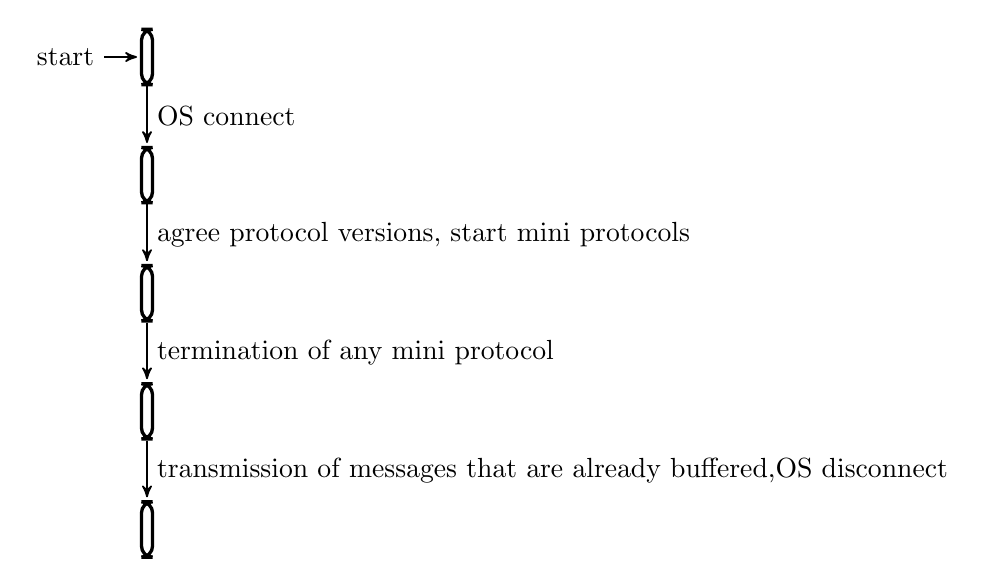
\begin{tikzpicture}[->,>=stealth',shorten >=1pt,auto,node distance=1.5cm, semithick]
  \tikzstyle{every state}=[fill=red,draw=none,text=white]
  \node[state, initial]                           (Larval)       {\Larval};
  \node[state, below of=Larval]                   (Connected)    {\Connected};
  \node[state, below of=Connected]                (Mature)       {\Mature};
  \node[state, below of=Mature]                   (Dying)        {\Dying};
  \node[state, below of=Dying]                    (Dead)         {\Dead};
  \draw (Larval)            edge[]      node{OS connect}         (Connected);
  \draw (Connected)         edge[]      node{agree protocol versions, start mini protocols}    (Mature);
  \draw (Mature)         edge[]      node{termination of any mini protocol}           (Dying);
  \draw (Dying)         edge[]      node{transmission of messages that are already buffered,OS disconnect}
         (Dead);
\end{tikzpicture}

A connection passes through several stages during its life cycle.
\begin{description}
\item[\Larval]    The connection exists but nothing has been initialised yet.
\item[\Connected] The OS-level primitives (sockets or pipes) are connected.
\item[\Mature] The mini protocols are running.
\item[\Dying]  One of the mini protocols has terminated.
\item[\Dead] The connection has been terminated.
\end{description}

\newcommand{\InitReq}{\msg{InitReq}}
\newcommand{\InitRsp}{\msg{InitRsp}}
\newcommand{\InitFail}{\msg{InitFail}}

\noindent\hsref{ouroboros-network/src/Ouroboros/Network/Mux/Types.hs}
\newline\hsref{ouroboros-network/src/Ouroboros/Network/NodeToNode.hs}
\newline\hsref{ouroboros-network/src/Ouroboros/Network/NodeToClient.hs}
\hide{Update needed !}
\begin{table}[ht]
\centering
\begin{tabular}{|l|l|l|l|}
  \hline
  ID & Mini Protocol                         & NtN  & NtC \\ \hline
  0  & MUX-Control                           & Yes  & Yes \\ \hline
  1  & DeltaQ                                & Yes  & Yes \\ \hline
  2  & Chain-Sync instantiated to headers    & Yes  & No \\ \hline
  3  & Block-Fetch                           & Yes  & No  \\ \hline
  4  & Transaction-Submission                & No   & Yes  \\ \hline
  5  & Chain-Sync instantiated to blocks     & No   & Yes  \\ \hline
\end{tabular}
\caption{Mini Protocol IDs}
\label{mini-protocol-id}
\end{table}

\subsection{Default Mini Protocol Sets for Node-to-Node and Node-to-Client}
Table~\ref{mini-protocol-id} show which mini protocols are enabled for node-to-node
and node-to-client communication.
Mux-Control and DeltaQ are enabled for all connections.
The communication between two full nodes (NtN) is fully symmetric.
Both nodes run initiator and responder instances of the
Chain-Sync, the Block-Fetch and the Transaction-Submission protocol.
Node-to-Client (NtC) is a connection between a full node and a client that does not take part in
Ouroboros protocol itself and only consumes data, for example a wallet or a block chain explorer.
In a NtC setup, the node only runs the producer side of the Chain-Sync protocol and the client only the
consumer side.
The Chain-Sync protocol is polymorphic in the type of blocks that are transmitted.
NtN uses a Chain-Sync instance which only transmits block headers, while the NtC instance transmits
full blocks.
The two variants of Chain-Sync use different protocol IDs.


\subsection{Error Handling}
When a mini protocol thread detects that a peer violates the mini protocol it throws an exception.
The MUX-layer catches the exceptions from the mini protocol threads and shuts down the connection.

\chapter{Mini Protocols}
\label{state-machine-section}

\section{Mini Protocols and Protocol Families}
A mini protocol is a well defined and modular building block of
the network protocol.
Structuring the protocol around mini protocols helps to manage the overall complexity of
the design and adds useful flexibility.
The design turns into a family of mini protocols that can be specialised to particular requirements
by choosing a particular set of mini protocols.

The mini protocols in this section describe both the initiator and responder of a communication.
The initiator is the dual of the responder and vice versa.
(The terms client/server and consumer/producer are also used sometimes.)
At any time a node will typically run many instances of mini protocols, including many instances of the
same mini protocol.
Each mini protocol instance of the node communicates with the dual
instance of exactly one peer.
All mini protocols that communicate with the same peer
share a single communication channel (pipe or socket)
and a multiplexer/de-multiplexer is used to multiplex the protocols over that channel.
Section~\ref{multiplexing-section} describes the multiplexing layer.

The set of mini protocols that run on a connection between two participants of the system
depends on the role of the participants, i.e. whether the node acts as a full node or just
a block chain consumer, for example a wallet.
\wip{
Section~\ref{peer-setup-section} describes how a connection between two nodes
that run a set of mini protocols is set up.
}

\section{Protocols as State Machines}
The implementation of the mini protocols uses a generic framework for state machines.
\hide{
The Haskell implementation of the state machine framework is described in
Section~\ref{Haskell-state-machine}.
}
This framework uses correct-by-construction techniques to guarantee
several properties of the protocol and the implementation.
In particular, it guarantees that there are no deadlocks.
At any time, one side has agency
(is expected to transmit the next message) and the other side is awaiting for
the message (or both sides agree that the protocol has terminated).
If either side receives a message that is not expected according to the protocol
the communication is aborted.

For each mini protocol that is based on this underlying framework the description provides the
following pieces of information:

\begin{itemize}
\item An informal description of the protocol.
\item States of the state machine.
\item The messages that are exchanged.
\item A transition graph of the global view of the state machine.
\item The client implementation of the protocol.
\item The server implementation of the protocol.
\end{itemize}

\begin{description}
\item[State Machine]
  Each mini protocol is described as a state machine.
  This document uses a simple diagram representations for state machines, and
  also includes corresponding transition tables.
  Descriptions of state machines in this section are directly derived from
  specifications of mini protocols using the state machine framework.

  The state machine framework that is used to specify the protocol can be instantiated
  with different implementations that work at different levels of abstraction
  (for example implementations used for simulation, implementations that run over virtual
  connections and implementations that actually transmit messages over the real network).


\item[States]
  States are abstract: they are not a value of some variables in a node, but
  rather describe the state of the two-party communication as whole, e.g.
  that a client is responsible for sending a particular type of message and
  the server is awaiting on it.  This, in particular, means that if the state
  machine is in a given state, both client and server are in this state.
  An additional piece of information that differentiates the roles of peers in
  a given state is agency, which describes which side is responsible for
  sending the next message.

  In the state machine framework, abstract states of a state machine are
  modelled as promoted types, so they do not correspond to any particular
  value hold by one of the peers.

  The document presents this abstract view of mini protocols and the state
  machines where the client and server are always in identical states, which
  also means that client and server simultaneously transit to new states.
  For this description network delays are not important.

  An interpretation, which is closer to the real-world implementation but
  less concise, is that there are independent client and server states
  and that transitions on either side happen independently when a message is sent or received.

\item[Messages]
  Messages exchanged by peers form edges of a state machine diagram, in other
  words they are transitions between states.
  They are elements from the set
  $$\{(label, data) \mid label \in Labels, data \in Data\}$$
  Protocols use a small set of $Labels$ typically $|Labels| \leq 10$.
  The state machine framework requires that messages can be serialised,
  transferred over the network and de-serialised by the receiver.
  The binary format for messages is described in appendix~\ref{CBOR-section}.

\item[Agency]
  A node has agency if it is expected to send the next message.
  In every state (except the \StDone-state) either the client or server has agency.
  In the \StDone-state the protocol has terminated and neither side is expected to send any more
  messages.

\item [State machine diagrams]
      States are drawn as circles in state machine diagrams.
      States with agency at the client are drawn in green, states with agency at the server in blue and
      the \StDone-state in black.
      By construction, the system is always in exactly one state,
      i.e. the client's state is always the same state as server's,
      and the colour indicates who is the agent.
      It is also important to understand that the arrows in the state transition diagram denote
      state transitions and not the direction of the message that is being transmitted.
      For the agent of the particular state the arrow means: ``send a message to the
      other peer and move to the next state''.
      For a non-agent an arrow in the diagram can be interpreted as:
      ``receive an incoming message and move to the next state''.
      This may be confusing because the arrows are labelled with the messages and
      many arrows go from a green state (client has the agency) to a blue
      state (server has the agency) or vice versa.

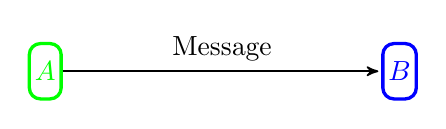
\begin{tikzpicture}[->,>=stealth',shorten >=1pt,auto,node distance=4.5cm, semithick]
  \tikzstyle{every state}=[fill=red,draw=none,text=white]
  \node[state, green]              (A)      {$A$};
  \node[state, blue ,right of=A]   (B)      {$B$};
  \draw (A)            edge[above]          node{Message}   (B);
\end{tikzpicture}

      $A$ is green, i.e in state $A$ the client has agency.
      Therefore the client sends a message to the server and
      both client and server transition to state $B$.
      As $B$ is blue the agency also changes from client to server.

\begin{tikzpicture}[->,>=stealth',shorten >=1pt,auto,node distance=4.5cm, semithick]
  \tikzstyle{every state}=[fill=red,draw=none,text=white]
  \node[state, blue]               (C)      {$C$};
  \node[state, blue ,right of=A]   (D)      {$D$};
  \draw (A)            edge[above]               node{Message}   (B);
\end{tikzpicture}

      $C$ is blue, i.e in state $C$ the server has agency.
      Therefore the server sends a message to the client and
      both client and server transition to state $D$.
      As $D$ is also blue the agency remains at the server.

\item[Client and server implementation]
  The state machine describes which messages are sent and received and in which order.
  This is the external view of the protocol that every compatible implementation MUST follow.
  In addition to the external view of the protocol, this part of the specification describes
  how the client and server actually process the transmitted messages,
  i.e. how the client and server update their internal mutable state
  upon the exchange of messages.

  Strictly speaking, the representation of the node-local mutable state
  and the updates to the node-local state are implementation details that are
  not part of the communication protocol between the nodes,  and will
  depend on an application that is built on top of the network service
  (wallet, core node, explorer, etc.).
  The corresponding sections were added to clarify the mode of operation of the
  mini protocols.

\end{description}
\section{Overview of all implemented Mini Protocols}

\newcommand{\miniEntry}[5]{
  \begin{framed}
      \noindent\textbf{#1}\hfill  Section \ref{#2}
      \newline {#3}
      \newline {\href{#5}{\small\texttt{#4}}}
  \end{framed}
}

\miniEntry
    {Ping Pong Protocol}
    {ping-pong-protocol}
    {A simple ping-pong protocol for testing.}
    {typed-protocols/src/Network/TypedProtocol/PingPong/Type.hs}
    {https://input-output-hk.github.io/ouroboros-network/typed-protocols-examples/Network-TypedProtocol-PingPong-Type.html\#t:PingPong}

\miniEntry
    {Request Response Protocol}
    {request-response-protocol}
    {A ping pong like protocol which allows to exchanges data.}
    {typed-protocols/src/Network/TypedProtocol/ReqResp/Type.hs}
    {https://input-output-hk.github.io/ouroboros-network/typed-protocols-examples/Network-TypedProtocol-ReqResp-Type.html\#t:ReqResp}

\miniEntry
    {Handshake Mini Protocol}
    {handshake-protocol}
    {This protocol is used for version negotiation.}
    {ouroboros-network/src/Ouroboros/Network/Protocol/Handshake/Type.hs}
    {https://input-output-hk.github.io/ouroboros-network/ouroboros-network-framework/Ouroboros-Network-Protocol-Handshake-Type.html\#t:Handshake}

\miniEntry
    {Chain Synchronisation Protocol}
    {chain-sync-protocol}
    {The protocol by which a downstream chain consumer follows an upstream chain producer.}
    {ouroboros-network/src/Ouroboros/Network/Protocol/ChainSync/Type.hs}
    {https://input-output-hk.github.io/ouroboros-network/ouroboros-network/Ouroboros-Network-Protocol-ChainSync-Type.html\#t:ChainSync}

\miniEntry
    {Block Fetch Protocol}
    {block-fetch-protocol}
    {The block fetching mechanism enables a node to download ranges of blocks.}
    {ouroboros-network/src/Ouroboros/Network/Protocol/BlockFetch/Type.hs}
    {https://input-output-hk.github.io/ouroboros-network/ouroboros-network/Ouroboros-Network-Protocol-BlockFetch-Type.html\#t:BlockFetch}

\miniEntry
    {Transaction Submission Protocol v2}
    {tx-submission-protocol2}
    {A Protocol for transmitting transaction between core nodes.}
    {ouroboros-network/src/Ouroboros/Network/Protocol/TxSubmission2/Type.hs}
    {https://input-output-hk.github.io/ouroboros-network/ouroboros-network/Ouroboros-Network-Protocol-TxSubmission2-Type.html\#t:TxSubmission2}

\miniEntry
    {Keep Alive Protocol}
    {keep-alive-protocol}
    {A protocol for sending keep alive messages and round trip measurments}
    {ouroboros-network/src/Ouroboros/Network/Protocol/KeepAlive/Type.hs}
    {https://input-output-hk.github.io/ouroboros-network/ouroboros-network/Ouroboros-Network-Protocol-KeepAlive-Type.html\#t:KeepAlive}


\miniEntry
    {Local Transaction Submission Mini Protocol}
    {local-tx-submission-protocol}
    {Transmitting Transactions from a wallet to a local node.}
    {ouroboros-network/src/Ouroboros/Network/Protocol/LocalTxSubmission/Type.hs}
    {https://input-output-hk.github.io/ouroboros-network/ouroboros-network/Ouroboros-Network-Protocol-LocalTxSubmission-Type.html\#t:LocalTxSubmission}

\miniEntry
    {Locat State Query Mini Protocol}
    {local-state-query-protocol}
    {Protocol used by local clients to query ledger state}
    {ouroboros-network/src/Ouroboros/Network/Protocol/LocalStateQuery/Type.hs}
    {https://input-output-hk.github.io/ouroboros-network/ouroboros-network/Ouroboros-Network-Protocol-LocalStateQuery-Type.html\#t:LocalStateQuery}

\section{CBOR and CDDL}
All mini-protocols are encoded using coincise binary object representation
(CBOR), see~\url{https://cbor.io}.  Each codec comes along with a specification
written in CDDL,
see~\url{https://cbor-wg.github.io/cddl/draft-ietf-cbor-cddl.html}.

\section{Dummy Protocols}
Dummy protocols are only used for testing and are not needed either for
Node-to-Node nor for the Node-to-Client protocols.
\subsection{Ping-Pong Protocol}
\label{ping-pong-protocol}
\haddockref{Network.TypedProtocol.PingPong.Type}{typed-protocols-examples/Network-TypedProtocol-PingPong-Type\#t:PingPong}
\newcommand{\Ping}{\msg{MsgPing}}
\newcommand{\Pong}{\msg{MsgPong}}


\subsubsection{Description}
A client can use the Ping-Pong protocol to check that the server is responsive.
The Ping-Pong protocol is very simple because the messages do not carry any data and
because the Ping-Pong client and the Ping-Pong server do not access the internal state of the node.

\subsubsection{State Machine}
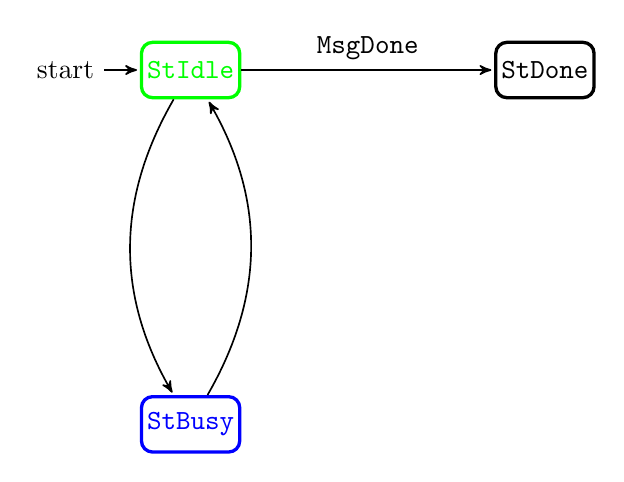
\begin{tikzpicture}[->,>=stealth',shorten >=1pt,auto,node distance=4.5cm, semithick]
  \tikzstyle{every state}=[fill=red,draw=none,text=white]
  \node[state, green, initial]                            (Idle)      {\StIdle};
  \node[state, right of=Idle]                             (Done)      {\StDone};
  \node[state, blue, below of=Idle]                       (Busy)      {\StBusy};

  \draw (Idle)         edge[above]               node{\MsgDone}                  (Done);
  \draw (Idle)         edge[left, bend right]    node{\Ping}                     (Busy);
  \draw (Busy)         edge[right, bend right]   node{\Pong}                     (Idle);
\end{tikzpicture}

\begin{figure}[ht]
\begin{tabular}{|l|l|} \hline
\multicolumn{2}{|c|}{Agency} \\ \hline
  Client has Agency & \StIdle \\  \hline
  Server has Agency & \StBusy \\  \hline
\end{tabular}
\end{figure}

The protocol uses the following messages.
The messages of the Ping-Pong protocol do not carry any data.
\begin{description}
\item [\Ping]
      The client sends a Ping request to the server.
\item [\Pong]
      The server replies to a Ping with a Pong.
\item [\MsgDone]
      Terminate the protocol.
\end{description}

\begin{tabular}{|l|l|l|}
  \hline
  \multicolumn{3}{|c|}{Transition table} \\ \hline
  from state   & message            & to state    \\ \hline\hline
  \StIdle        & \Ping              & \StBusy   \\ \hline
  \StBusy        & \Pong              & \StIdle   \\ \hline
  \StIdle        & \MsgDone           & \StDone       \\ \hline
\end{tabular}

\subsection{Request Response Protocol}
\label{request-response-protocol}
\haddockref{Network.TypedProtocol.ReqResp.Type}{typed-protocols-examples/Network-TypedProtocol-ReqResp-Type.html\#t:ReqResp}
\renewcommand{\StIdle}{\state{StIdle}}
\renewcommand{\StBusy}{\state{StBusy}}
\renewcommand{\StDone}{\state{StDone}}
\newcommand{\Request}{\msg{MsgReq}}
\newcommand{\Response}{\msg{MsgResp}}
\newcommand{\RespDone}{\msg{MsgDone}}

\subsubsection{Description}
The request response protocol is polymorphic in the request and response data that is being transmitted.
This means that there are different possible applications of this protocol and the
application of the protocol determines the types of the requests and responses.

\subsubsection{State machine}
\begin{tabular}{|l|l|}
  \hline
  \multicolumn{2}{|c|}{Agency} \\ \hline
  Client has Agency & \StIdle \\  \hline
  Server has Agency & \StBusy \\ \hline
\end{tabular}
{\vskip 10pt}
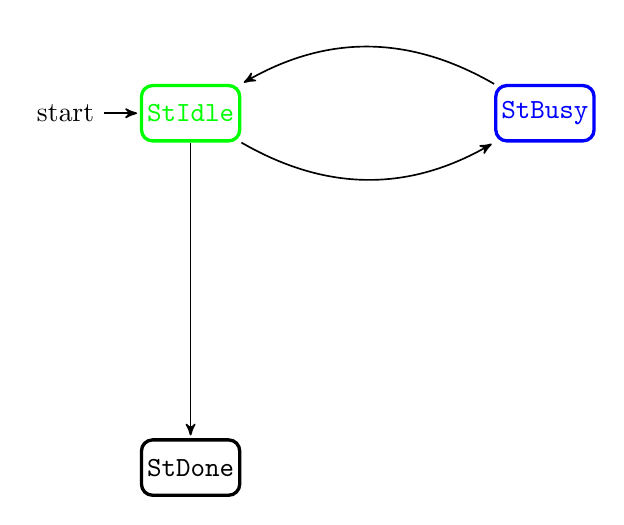
\begin{tikzpicture}[->,>=stealth',shorten >=1pt,auto,node distance=4.5cm, semithick]
  \tikzstyle{every state}=[fill=red,draw=none,text=white]
  \node[state, green, initial]                                   (Idle)      {\StIdle};
  \node[state, blue, right of=Idle]                              (Busy)      {\StBusy};
  \node[state, below of=Idle]                                    (Done)      {\StDone};

  \draw (Idle)         edge[below, bend right] node{\Request}    (Busy);
  \draw (Busy)         edge[above, bend right] node{\Response}   (Idle);
  \draw (Idle)         edge[right]             node{\RespDone}   (Done);
\end{tikzpicture}
{\vskip 10pt}
The protocol uses the following messages.
\begin{description}
\item [\Request{} $(request)$]
      The client sends a request to the server.
\item [\Response{} $(response)$]
      The server replies with a response.
\item [\RespDone{} $(done)$]
      Terminate the protocol.
\end{description}

\begin{tabular}{|l|l|l|l|} \hline
\multicolumn{4}{|c|}{Transition table} \\ \hline
  from           & message            & parameters             & to          \\ \hline\hline
  \StIdle        & \Request           & $request$              & \StBusy     \\ \hline
  \StBusy        & \Response          & $response$             & \StIdle     \\ \hline
  \StIdle        & \RespDone          &                        & \StDone     \\ \hline
\end{tabular}

\section{Handshake Mini Protocol}
\haddockref{Ouroboros.Network.Protocol.Handshake.Type}{ouroboros-network-framework/Ouroboros-Network-Protocol-Handshake-Type\#t:Handshake}
\label{handshake-protocol}
\newcommand{\StPropose}{\state{StPropose}}
\newcommand{\StConfirm}{\state{StConfirm}}
\newcommand{\MsgProposeVersions}{\msg{MsgProposeVersions}}
\newcommand{\MsgAcceptVersion}{\msg{MsgAcceptVersion}}
\newcommand{\MsgRefuse}{\msg{MsgRefuse}}

\newcommand{\VersionMismatch}{\msg{VersionMismatch}}
\newcommand{\HandshakeDecodeError}{\msg{HandshakeDecodeError}}
\newcommand{\Refused}{\msg{Refused}}

\subsection{Description}
The handshake mini protocol is used to negotiate the protocol version
and the protocol parameters that are used by the client and the server.
It is run exactly once when a new connection is initialised
and consists of a single request from the client and a single reply from the server.
Section \ref{peer-setup-section} explains the live cycle of a connection and the role of
the handshake mini protocol in more detail.

The handshake mini protocol is a generic protocol that can negotiate any kind protocol parameters.
It only assumes that protocol parameters can be encoded to, and decoded from, CBOR terms.
A node, that runs the handshake protocol, must instantiate it with the set of
supported protocol versions and callback functions for handling the protocol parameters.
These callback functions are specific for the supported protocol versions.

\subsection{State machine}

\begin{tabular}{|l|l|}
  \hline
  \multicolumn{2}{|c|}{Agency} \\ \hline
  Client has Agency & \StPropose \\ \hline
  Server has Agency & \StConfirm \\  \hline
\end{tabular}

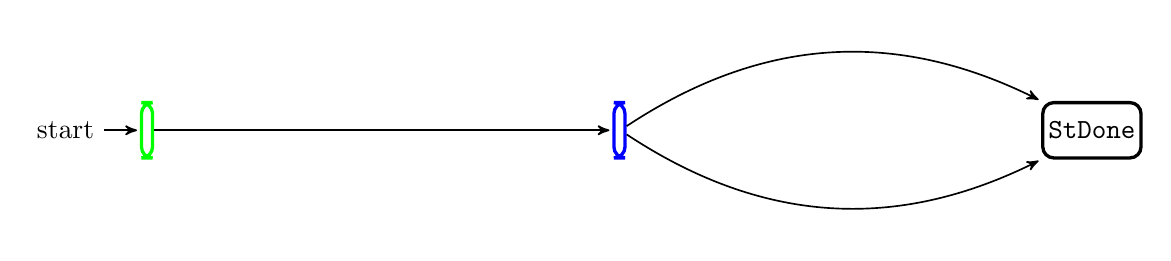
\begin{tikzpicture}[->,>=stealth',shorten >=1pt,auto,node distance=6cm, semithick]
  \tikzstyle{every state}=[fill=red,draw=none,text=white]
  \node[state, green, initial]                                     (Propose)    {\StPropose};
  \node[state, blue, right of=Propose]                             (Confirm)    {\StConfirm};
  \node[state, right of=Confirm]                                   (Done)       {\StDone};

  \draw (Propose)      edge[]      node{\MsgProposeVersions}          (Confirm);
  \draw (Confirm)      edge[above, bend left]       node{\MsgAcceptVersion}     (Done);
  \draw (Confirm)      edge[below, bend right]      node{\MsgRefuse}            (Done);

\end{tikzpicture}

Messages of the protocol:
\begin{description}
\item [\MsgProposeVersions{} {\boldmath $(versionTable)$}]
      The client proposes a number of possible versions and protocol parameters.
\item [\MsgAcceptVersion{} {\boldmath $(versionNumber,extraParameters)$}]
      The server accepts $versionNumber$ and returns possible extra protocol parameters.
\item [\MsgRefuse{} {\boldmath $(reason)$}]
      The server refuses the proposed versions.
\end{description}

\begin{tabular}{|l|l|l|l|} \hline
\multicolumn{4}{|c|}{Transition table} \\ \hline
  from        & message/event      & parameters                   & to          \\ \hline\hline
  \StPropose    & \MsgProposeVersions   & $versionTable$          & \StConfirm    \\ \hline
  \StConfirm    & \MsgAcceptVersion     & $(versionNumber,extraParameters)$ & \StDone \\ \hline
  \StConfirm    & \MsgRefuse            & $reason$                & \StDone \\ \hline
\end{tabular}

\subsection{Client and Server Implementation}
Section~\ref{handshake-cddl} contains the CDDL-specification of the binary format of the handshake messages.
The version table is encoded as a CBOR table with the version number as key
and the protocol parameters as value.
The handshake protocol requires that the version numbers ( i.e. the keys) in the version table are unique
and appear in ascending order.
(Note, that CDDL is not expressive enough to precisely specify that requirement on the keys of the CBOR
table. Therefor the CDDL-specification uses a table with keys from 1 to 4 as an example.)

In a run of the handshake mini protocol the peers exchange only two messages:
The client requests to connect with a \MsgProposeVersions{} message that contains information about
all protocol versions it wants to support.
The server replies either with an \MsgAcceptVersion{} message containing the negotiated
version number and extra parameters or a \MsgRefuse{} message.
The \MsgRefuse{} message contains one of three alternative refuse reasons:
\VersionMismatch{}, \HandshakeDecodeError{} or just \Refused{}.

When a server receives a \MsgProposeVersions{} message it uses the following algorithm to
compute the response:
\begin{enumerate}
\item
  Compute the intersection of the set of protocol version numbers that the server support
  and the version numbers requested by the client.
\item
  If the intersection is empty:
  Reply with \MsgRefuse(\VersionMismatch) and the list of protocol numbers the server supports.
\item
  Otherwise:
  Select the protocol with the highest version number in the intersection.
\item
  Run the protocol specific decoder on the CBOR term that contains the protocol parameters.
\item
  If the decoder fails:
  Reply with \MsgRefuse(\HandshakeDecodeError), the selected version number and an error message.
\item
  Otherwise: Test the proposed protocol parameters of the selected protocol version
\item
  If the test refuses the parameters:
  Reply with \MsgRefuse(\Refused), the selected version number and an error message.
\item
  Otherwise:
  Encode the extra parameters and
  reply with \MsgAcceptVersion, the selected version number and the extra parameters.
\end{enumerate}
Note, that in step 4), 6) and 8) the handshake protocol uses the callback functions that are specific
for set of protocols that the server supports.
The handshake protocol is designed,
such that a server can always handle requests for protocol versions that it does not support.
The server simply ignores the CBOR terms that represent the protocol parameters of unsupported
version.

The handshake mini protocol runs before the MUX/DEMUX itself is initialised.
Each message is transmitted within a single MUX segment, i.e. with a proper
segment header, but, as the MUX/DEMUX is not yet running the messages must not
be split into multiple segments.  These MUX segments are using a reserved
protocol id $0$ (\texttt{Muxcontrol}).

\subsection{CDDL encoding specification}\label{handshake-cddl}
There are two flavours of the mini-protocol which only differ with type
instatiations, e.g. different protocol versions and version data carried in
messages.  First one is used by the node to node protocol the other by node to
client protocol.

\subsubsection{Node to node handshake mini-protocol}
\lstinputlisting[style=cddl]{../../ouroboros-network/test-cddl/specs/handshake-node-to-node.cddl}
\subsubsection{Node to client handshake mini-protocol}
\lstinputlisting[style=cddl]{../../ouroboros-network/test-cddl/specs/handshake-node-to-client.cddl}

\section{Chain-Sync Protocol}
\label{chain-sync-protocol}
\haddockref{Ouroboros.Network.Protocol.ChainSync.Type}{ouroboros-network/Ouroboros-Network-Protocol-ChainSync-Type\#t:ChainSync}
\newcommand{\StCanAwait}{\state{StCanAwait}}
\newcommand{\StMustReply}{\state{StMustReply}}
\newcommand{\StIntersect}{\state{StIntersect}}
\newcommand{\MsgRequestNext}{\msg{MsgRequestNext}}
\newcommand{\MsgAwaitReply}{\msg{MsgAwaitReply}}
\newcommand{\MsgRollForward}{\msg{MsgRollForward}}
\newcommand{\MsgRollBackward}{\msg{MsgRollBackward}}
\newcommand{\MsgFindIntersect}{\msg{MsgFindIntersect}}
\newcommand{\MsgIntersectFound}{\msg{MsgIntersectFound}}
\newcommand{\MsgIntersectNotFound}{\msg{MsgIntersectNotFound}}

\subsection{Description}
The chain synchronisation protocol is used by a block chain consumer
to replicate the producer's block chain locally.
A node communicates with several upstream and downstream nodes
and runs an independent client instance and a independent server instance for every
other node it communicates with.
(See Figure~\ref{node-diagram-concurrency}.)

The chain synchronisation protocol is polymorphic.
The (full)-node to client protocol uses an instance of the chain synchronisation protocol
that transfers full blocks, while the node-to-node instance only transfers block headers.
In the node-to-node case, the block fetch protocol (Section \ref{block-fetch-protocol})
is used to transfer full blocks.

\subsection{State Machine}

\begin{tabular}{|l|l|}
  \hline
  \multicolumn{2}{|c|}{Agency} \\ \hline
  Client has Agency & \StIdle \\  \hline
  Server has Agency & \StCanAwait, \StMustReply, \StIntersect \\ \hline
\end{tabular}

\begin{figure}[ht]
\begin{tikzpicture}[->,>=stealth',shorten >=1pt,auto,node distance=5.5cm, semithick]
  \tikzstyle{every state}=[fill=red,draw=none,text=white]
  \node[state, green, initial]                            (Idle)      {\StIdle};
  \node[state, right of=Idle]                             (Done)      {\StDone};
  \node[state, blue, below left of=Idle]                  (CanAwait)  {\StCanAwait};
  \node[state, blue, right of=CanAwait]                   (MustReply) {\StMustReply};
  \node[state, blue, above of=Idle]                       (Intersect) {\StIntersect};

  \draw (Idle)         edge[left, bend right]      node{\MsgRequestNext}           (CanAwait);
  \draw (CanAwait)     edge[below, bend right]     node{\MsgAwaitReply}            (MustReply);
  \draw (CanAwait)     edge[above,bend right=45]   node{\MsgRollForward}           (Idle);
  \draw (MustReply)    edge[right,bend right=45]   node{\MsgRollForward}           (Idle);
  \draw (CanAwait)     edge[above,bend right=80]   node{\MsgRollBackward}          (Idle);
  \draw (MustReply)    edge[right,bend right=80]   node{\MsgRollBackward}          (Idle);
  \draw (Idle)         edge[right, bend right]     node{\MsgFindIntersect}         (Intersect);
  \draw (Intersect)    edge[above, bend right=45]  node[below = 4mm]{\MsgIntersectFound}     (Idle);
  \draw (Intersect)    edge[above, bend right=80]  node[above = 4mm]{\MsgIntersectNotFound}  (Idle);
  \draw (Idle)         edge[above]                 node{\MsgDone}                  (Done);
\end{tikzpicture}
\caption{State machine of the chain sync protocol.}
\label{chain-sync-automata}
\end{figure}

The protocol uses the following messages:
\begin{description}
\item [\MsgRequestNext]
      Request the next update from the producer.
\item [\MsgAwaitReply]
      Acknowledge the request but require the consumer to wait for the next update.
      This means that the consumer is synced with the producer, and
      the producer is waiting for its own chain state to change.
\item [\MsgRollForward{} {\boldmath $(header, tip)$}]
      Tell the consumer to extend their chain with the given $header$.
      The message also tells the consumer about the $tip$ of the producers chain.
\item [\MsgRollBackward{} {\boldmath $(point_{old}, tip$}]
      Tell the consumer to roll back to a given $point_{old}$ on their chain.
      The message also tells the consumer about the current  $tip$ of the chain the producer is following.
\item [\MsgFindIntersect{} {\boldmath $\langle point_{head} \rangle $}]
      Ask the producer to try to find an improved intersection point between
      the consumer and producer's chains.
      The consumer sends a sequence {\boldmath $\langle point \rangle $}
      and it is up to the producer
      to find the first intersection point on its chain and send it back to the consumer.
\item [\MsgIntersectFound{} {\boldmath $(point_{intersect} ,tip)$}]
      The producer replies with the first point of the request that is on his current chain.
      The consumer can decide whether to send more points.
      The message also tells the consumer about the $tip$ of the producer.
\item [\MsgIntersectNotFound{} {\boldmath $(tip)$}]
      The reply to the consumer that no intersection was found: none of the
      points the consumer supplied are on the producer chain.
      The message only contains the $tip$ of the producer chain.
\item [\MsgDone]
      Terminate the protocol.
\end{description}

\begin{tabular}{|l|l|l|l|}
  \hline
  \multicolumn{4}{|c|}{Transition table} \\ \hline
  from state & message             & parameters                          & to state    \\ \hline\hline
  \StIdle      & \MsgRequestNext        &                                     & \StCanAwait   \\ \hline
  \StIdle      & \MsgFindIntersect      & $\langle point\rangle$              & \StIntersect  \\ \hline
  \StIdle      & \MsgDone            &                                     & \StDone       \\ \hline
  \StCanAwait  & \MsgAwaitReply         &                                     & \StMustReply  \\ \hline
  \StCanAwait  & \MsgRollForward        & $header$, $tip$                     & \StIdle       \\ \hline
  \StCanAwait  & \MsgRollBackward       & $header_{old}$, $tip$                & \StIdle       \\ \hline
  \StMustReply & \MsgRollForward        & $header$, $tip$                     & \StIdle       \\ \hline
  \StMustReply & \MsgRollBackward       & $point_{old}$, $tip$                 & \StIdle       \\ \hline
  \StIntersect & \MsgIntersectFound     & $point_{intersect}$, $tip$            & \StIdle       \\ \hline
  \StIntersect & \MsgIntersectNotFound  & $tip$                               & \StIdle       \\ \hline

\end{tabular}

\newcommand{\readpointer}{\emph{read-pointer}}
\subsection{Implementation of the Chain Producer}
\hide{The trade-offs between the robustness and efficiency of possible chain-sync protocols are
discussed in Section~\ref{chain-sync-discussion}.
}
This section describes a state-full implementation of a chain producer that is suitable for a setting where
the producer cannot trust the chain consumer.
An important requirement in this setting
is that a chain consumer must never be able to cause excessive resource use on the producer side.
The presented implementation meets this requirement.
It uses a constant amount of memory to store the state that the producer maintains
per chain consumer.  This protocol is only used to reproduce the producer
chain locally by consumer.  By running many instances of this protocol against
different peers, a node can reproduce chains in the network and
do chain selection which by design is not part of this protocol.
Note, that when we refer to the consumer's chain in this section, we mean
the chain that is reproduced by the consumer with the instance of
the chain-sync protocol under consideration and not the result of the chain selection algorithm.

We call the state which the producer maintains about the consumer the \readpointer{}.
The \readpointer{} basically tracks what the producer knows about the head of
the consumer's chain without storing it locally.
It points to a block on the current chain of the chain producer.
The \readpointer{}s are part of the shared state of the node (Figure~\ref{node-diagram-concurrency}) and
\readpointer{}s are concurrently updated by the thread that runs the chain-sync mini-protocol and the
chain tracking logic of the node itself.

We first describe how the mini-protocol updates a \readpointer{} and later address what happens in case
of a fork.
\subparagraph{Initializing the \readpointer{}.}
The chain producer assumes that a consumer, which has just connected,
only knows the genesis block and initialises the \readpointer{} of that consumer
with a pointer to the genesis block on its chain.

\subparagraph{Downloading a chain of blocks}
A typical situation is when the consumer follows the chain of the producer but is not yet at the head of the
chain (this also covers a consumer booting from genesis).
In this case, the protocol follows a simple, consumer-driven, request-response pattern.
The consumer sends \MsgRequestNext{} messages to ask for the next block.
If the \readpointer{} is not yet at the head of the chain,
the producer replies with a \MsgRollForward{} and advances the \readpointer{} to
the next block (optimistically assuming that the client will update its chain
accordingly).
The \MsgRollForward{} message contains the next block and also the head-point of the producer.
The protocol follows this pattern until the \readpointer{} reaches the end of its chain.

\begin{figure}[ht]
\pgfdeclareimage[height=7cm]{read-pointer-consumer-driver}{figure/read-pointer-consumer-driven.pdf}
\begin{center}
\pgfuseimage{read-pointer-consumer-driver}
\end{center}
\caption{Consumer driven block download.}
\label{read-pointer-consumer-driver}
\end{figure}

\subparagraph{Producer driven updates}
If the \readpointer{} points to the end of the chain and the producer receives
a \MsgRequestNext{}
the consumers chain is already up to date.
The producer informs the consumer with an \MsgAwaitReply{} that no new data is available.
After receiving a \MsgAwaitReply, the consumer just waits for a new message and the producer keeps agency.
The \MsgAwaitReply{} switches from a consumer driven phase to a producer driven phase.

The producer waits until new data becomes available.
When a new block is available, the producer will
send a \MsgRollForward{} message and give agency back to the consumer.
The producer can also get unblocked when its node switches to a new chain fork.

\subparagraph{Producer switches to a new fork}
The node of the chain producer can switch to a new fork at any time, independent of the
state machine.
A chain switch can cause an update of the \readpointer{},
which is part of the mutable state that is shared between the thread that runs
the chain sync protocol and the thread that implements the chain following logic of the node.
There are two cases:

1) If the \readpointer{} points to a block that is on the common prefix of the new
fork and the old fork, no update of the \readpointer{} is needed.

2) If the \readpointer{} points to a block that is no longer part of the chain that is followed by the node,
the \readpointer{} is set to the last block that is common between the new and the old chain.
The node also sets a flag that signals the chain-sync thread to send a \MsgRollBackward{} instead
of a \MsgRollForward.
Finally the producer thread must unblock if it is in the \StMustReply{} state.

\begin{figure}[ht]
\pgfdeclareimage[height=5cm]{read-pointer-rollback}{figure/read-pointer-rollback.pdf}
\begin{center}
\pgfuseimage{read-pointer-rollback}
\end{center}
\caption{\readpointer{} update for a fork switch in case of a rollback.}
\label{read-pointer-rollback}
\end{figure}

Figure~\ref{read-pointer-rollback} illustrates a fork switch that requires an update of the \readpointer{}
for one of the chain consumers, i.e. an example for case 2.
Before the switch, the \readpointer{} of the consumer points to block $0x660f$.
The producer switches to a new chain with the head of the chain at block $0xcdf0$.
The node must update the \readpointer{} to block $0xfa40$ and the next message to the consumer
will be a \MsgRollBackward.

Note, that a node typically communicates with several consumers. For each consumer it runs an independent
version of the chain-sync-protocol state machine in an independent thread and with its own \readpointer{}.
Each of those \readpointer{}s has to be updated independently and for each consumer
either case 1) or case 2) can apply.

\subparagraph{Consumer starts with an arbitrary fork}
Typically, the consumer already knows some fork of the block chain when it
starts to track the producer.
The protocol provides an efficient method to search for the longest common prefix (here called intersection)
between the fork of the producer and the fork that is known to the consumer.

To do so, the consumer sends a \MsgFindIntersect{} message with a list of chain
points on the chain known to the consumer.
If the producer does not know any of the points it replies with \MsgIntersectNotFound.
Otherwise it replies with \MsgIntersectFound{} and the best (i.e. the newest) of the points that it knows
and also updates the \readpointer{} accordingly.
For efficiency, the consumer should use a binary search scheme to search for the longest common
prefix.

It is advised that the consumer always starts with \MsgFindIntersect{} in a fresh connection
and it is free to use \MsgFindIntersect{} at any time later as seems beneficial.
If the consumer does not know anything about the producer's chain,
it can start the search with the following list of points:
$\langle point(b), point(b-1), point(b-2), point(b-4), point (b-8),\ldots \rangle$
where $point(b-i)$ is the point of the $i$th predecessor of block $b$ and
$b$ is the head of the consumer fork.
Maximum depth of a fork in Ouroboros is bounded and the intersection will always be found with a small number of
iterations of this algorithm.

\subsection{Implementation of the Chain Consumer}
In principle, the chain consumer has to guard against a malicious chain producer
as much as the other way around.
However, two aspects of the protocol play in favour of the consumer here.
\begin{itemize}
  \item The protocol is basically consumer driven, i.e. the producer has no way to send unsolicited
data to the consumer (within the protocol).
  \item The consumer can verify the response data itself.
\end{itemize}
Here are some cases to consider:
\begin{description}
\item[\MsgFindIntersect~Phase]
  The consumer and the producer play a number guessing game, so the consumer can easily detect
  inconsistent behaviour.
\item[The producer replies with a \MsgRollForward] The consumer can verify the block itself
  with the help of the ledger layer.
  (The consumer may need to download the block first, if the protocol only sends block headers.)
\item[The producer replies with a \MsgRollBackward] The consumer tracks several producers, so
  if the producer sends false \MsgRollBackward{} messages the consumer's node
  will, at some point, just switch to a longer chain fork.
\item[The Producer is just passive/slow] The consumer's node will switch to
  a longer chain coming from another producer via another instance of
    chain-sync protocol.
\end{description}

\subsection{CDDL encoding specification}
\lstinputlisting[style=cddl]{../../ouroboros-network/test-cddl/specs/chain-sync.cddl}
See appendix \ref{cddl-common} for common definitions.

\section{Block Fetch Protocol}
\label{block-fetch-protocol}
\haddockref{Ouroboros.Network.Protocol.BlockFetch.Type}{ouroboros-network/Ouroboros-Network-Protocol-BlockFetch-Type\#t:BlockFetch}

\renewcommand{\StIdle}{\state{StIdle}}
\renewcommand{\StBusy}{\state{StBusy}}
\newcommand{\StStreaming}{\state{StStreaming}}
\renewcommand{\StDone}{\state{StDone}}
\newcommand{\MsgRequestRange}{\msg{MsgRequestRange}}
\newcommand{\MsgStartBatch}{\msg{MsgStartBatch}}
\newcommand{\MsgNoBlocks}{\msg{MsgNoBlocks}}
\newcommand{\MsgBlock}{\msg{MsgBlock}}
\newcommand{\MsgBatchDone}{\msg{MsgBatchDone}}
\newcommand{\MsgClientDone}{\msg{MsgClientDone}}

\subsection{Description}

The block fetching mechanism enables a node to download a range of blocks.

\subsection{State machine}

\begin{tabular}{|l|l|}
  \hline
  \multicolumn{2}{|c|}{Agency} \\ \hline
  Client has Agency & \StIdle            \\  \hline
  Server has Agency & \StBusy, \StStreaming \\ \hline
\end{tabular}

\begin{tikzpicture}[->,>=stealth',shorten >=1pt,auto,node distance=4.5cm, semithick]
  \tikzstyle{every state}=[fill=red,draw=none,text=white]
  \node[state, green,initial] at (-1cm,0cm)  (Idle)      {\StIdle};
  \node[state]                at (4cm,0cm)   (Done)      {\StDone};
  \node[state, blue]          at (-3cm,-3cm) (Busy)      {\StBusy};
  \node[state, blue]          at (4cm,-3cm)  (Streaming) {\StStreaming};

  \draw (Idle)         edge[above]                node{\MsgClientDone}                  (Done);
  \draw (Idle)         edge[left,bend right]      node{\MsgRequestRange}                (Busy);
  \draw (Busy)         edge[above,bend right]     node{\MsgNoBlocks}                    (Idle);
  \draw (Busy)         edge[below]                node{\MsgStartBatch}                  (Streaming);
  \draw (Streaming)    edge[loop right]           node{\MsgBlock}                       (Streaming);
  \draw (Streaming)    edge[right]                node{\MsgBatchDone}                   (Idle);
\end{tikzpicture}

\begin{description}
\item [\MsgRequestRange{} {\boldmath $(range)$}]
  The client requests a {\boldmath $range$} of blocks from the server.
\item [\MsgNoBlocks]
  The server tells the client that it does not have blocks.
\item [\MsgStartBatch]
  The server starts block streaming.
\item [\MsgBlock{} {\boldmath $(body)$}]
  Stream a single block's body.
\item [\MsgBatchDone]
  The server ends block streaming.
\item [\MsgClientDone]
  The client terminates the protocol.
\end{description}

Transition table:

\begin{tabular}{|l|l|l|l|}
  \hline
  \multicolumn{4}{|c|}{Transition table} \\ \hline
  from state   & message             & parameters             & to state    \\ \hline\hline
  \StIdle        & \MsgClientDone         &                        & \StDone       \\ \hline
  \StIdle        & \MsgRequestRange       & $range$                & \StBusy       \\ \hline
  \StBusy        & \MsgNoBlocks           &                        & \StIdle       \\ \hline
  \StBusy        & \MsgStartBatch         &                        & \StStreaming  \\ \hline
  \StStreaming   & \MsgBlock              & $body$                 & \StStreaming  \\ \hline
  \StStreaming   & \MsgBatchDone          &                        & \StIdle       \\ \hline
\end{tabular}

\subsection{CDDL encoding specification}
\lstinputlisting[style=cddl]{../../ouroboros-network/test-cddl/specs/block-fetch.cddl}
See appendix \ref{cddl-common} for common definitions.

\section{TxSubmission Protocol}
\subsection{Version 1}
\haddockref{Ouroboros.Network.Protocol.TxSubmission.Type}{ouroboros-network/Ouroboros-Network-Protocol-TxSubmission-Type\#t:TxSubmission}
\label{tx-submission-protocol}
\newcommand{\TxIdsBlocking}   {\state{StTxIdsBlocking}}
\newcommand{\TxIdsNonBlocking}{\state{StTxIdsNonBlocking}}
\newcommand{\Txs}             {\state{StTxs}}
\newcommand{\RequestTxIdsNB}  {\trans{MsgRequestTxIdsNonBlocking}}
\newcommand{\RequestTxIdsB}   {\trans{MsgRequestTxIdsBlocking}}
\newcommand{\ReplyTxIds}      {\trans{MsgReplyTxIds}}
\newcommand{\RequestTxs}      {\trans{MsgRequestTxs}}
\newcommand{\ReplyTxs}        {\trans{MsgReplyTxs}}

\subsubsection{Description}
The node-to-node transaction submission protocol is used to transfer transactions between full nodes.
The protocol follows a pull-based strategy where the initiator asks for new transactions and the responder
replies with the transactions.
It is suitable for a trustless setting where both sides need to guard against resource consumption attacks from
the other side.
The local transaction submission protocol, which is used when the server trusts a local client,
is described in Section \ref{local-tx-submission-protocol}.
The implementation of the node-to-node transaction mini protocol is based on a generic mini protocol framework
(the same as for all other mini protocols).
For technical reasons however the roles of the initiator and the responder are reversed with respect to
the way the other mini protocols are implemented in the frame work.
In other words: The Server is the initiator and ask for new transactions
and the Client is the responder and replies with the transactions.

The version 1 of the protocol is only used by the node-to-node protocol version
5 and earlier.
\subsubsection{State machine}

\begin{tabular}{|l|l|}
  \hline
  \multicolumn{2}{|c|}{Agency} \\ \hline
  Server has Agency & \StIdle \\  \hline
  Client has Agency & \TxIdsBlocking, \TxIdsNonBlocking, \Txs \\ \hline
\end{tabular}

\begin{figure}[h]
\begin{tikzpicture}[->,>=stealth',shorten >=1pt,auto,node distance=5.5cm, semithick]
  \tikzstyle{every state}=[fill=red,draw=none,text=white]
  \node[state, blue, initial](A) at ( 0,  0) {\StIdle};
  \node[state]               (B) at ( 8, -4) {\StDone};
  \node[state, green]        (C) at ( 4, -4) {\TxIdsBlocking};
  \node[state, green]        (D) at (-4, -4) {\TxIdsNonBlocking};
  \node[state, green]        (E) at ( 0,  4) {\Txs};
  \draw (C)  edge[above]                    node[below]{\MsgDone}                                 (B);
  \draw (A)  edge[left, bend left=45]       node[fill = white, anchor = center]{\RequestTxIdsB}   (C);
  \draw (C)  edge[right, bend left=15]      node[fill = white, anchor = center, above = 2pt]{\ReplyTxIds}     (A);
  \draw (A)  edge[right, bend left=15]      node[fill = white, anchor = center, below = 2pt]{\RequestTxIdsNB} (D);
  \draw (D)  edge[right, bend left=45]      node[fill = white, anchor = center]{\ReplyTxIds}      (A);
  \draw (A)  edge[left, bend right=45]      node[fill = white, anchor = center]{\RequestTxs}      (E);
  \draw (E)  edge[right,bend right=45]      node[fill = white, anchor = center]{\ReplyTxs}        (A);
\end{tikzpicture}
\caption{State machine of the transaction submission protocol.}
\label{tx-submission-automata}
\end{figure}
Messages of the protocol:
\begin{description}
\item [\RequestTxIdsB{} {\boldmath $(ack,req)$}]
      The server asks for new transaction ids and acknowledges old ids.
      The client will block until new transactions are available.
\item [\RequestTxIdsNB{} {\boldmath $(ack,req)$}]
      The server asks for new transaction ids and acknowledges old ids.
      The client immediately replies (possible with an empty list).
\item [\ReplyTxIds{} {\boldmath ($\langle (id, size) \rangle$) }]
      The client replies with a list of available transactions.
      The list contains pairs of transactions ids and the corresponding size of the transaction in bytes.
      In the blocking case the reply is guaranteed to contain at least one transaction.
      In the non-blocking case, the reply may contain an empty list.
\item [\RequestTxs{} {\boldmath ($\langle ids \rangle$)}]
      The server requests transactions by sending a list of transaction-ids.
\item [\ReplyTxs{} {\boldmath ($\langle txs \rangle$})]
      The client replies with a list transaction.
\item [\MsgDone]
      The client terminates the mini protocol.
\end{description}

\begin{tabular}{|l|l|l|l|}
  \hline
  \multicolumn{4}{|c|}{Transition table} \\ \hline
  from state        & message             & parameters                    & to state          \\ \hline\hline
  \StIdle             & \RequestTxIdsB      & $ack$,$req$                   & \TxIdsBlocking    \\ \hline
  \TxIdsBlocking    & \ReplyTxIds         & $\langle (id, size) \rangle$  & \StIdle             \\ \hline
  \StIdle             & \RequestTxIdsNB     & $ack$,$req$                   & \TxIdsNonBlocking \\ \hline
  \TxIdsNonBlocking & \ReplyTxIds         & $\langle (id, size) \rangle$  & \StIdle             \\ \hline
  \StIdle             & \RequestTxs         & $\langle ids \rangle$         & \Txs              \\ \hline
  \Txs              & \ReplyTxs           & $\langle txs \rangle$         & \StIdle             \\ \hline
  \RequestTxIdsB    & \MsgDone            &                               & \StDone             \\ \hline
\end{tabular}
\subsubsection{CDDL encoding specification}\label{tx-submission-cddl}
\lstinputlisting[style=cddl]{../../ouroboros-network/test-cddl/specs/tx-submission.cddl}
See appendix \ref{cddl-common} for common definitions.

\subsection{Version 2}
\haddockref{Ouroboros.Network.Protocol.TxSubmission2.Type}{ouroboros-network/Ouroboros-Network-Protocol-TxSubmission2-Type\#t:TxSubmission2}
\label{tx-submission-protocol2}
\newcommand{\Hello}  {\state{Hello}}
\newcommand{\MsgHello} {\trans{MsgHello}}

\subsubsection{Description}
This mini-protocol changes the initial state of the transaction submission
mini-protocol v1.  The new initial state, unlike the previous version, has
agency on the client side.  One the client initialises the mini-protocol
conversation with \MsgHello{} the version 1 of the protocol takes over.

The version 2 is used by version 6 of node-to-node protocol.
\subsubsection{State machine}

\begin{tabular}{|l|l|}
  \hline
  \multicolumn{2}{|c|}{Agency} \\ \hline
  Server has Agency & \StIdle \\  \hline
  Client has Agency & \TxIdsBlocking, \TxIdsNonBlocking, \Txs \\ \hline
\end{tabular}

\begin{figure}[h]
\begin{tikzpicture}[->,>=stealth',shorten >=1pt,auto,node distance=4.5cm, semithick]
  \tikzstyle{every state}=[fill=red,draw=none,text=white]
  \node[state, green, initial] (I) at (-4,  0) {\Hello};
  \node[state, blue]           (A) at ( 0,  0) {\StIdle};
  \node[state]                 (B) at ( 8, -4) {\StDone};
  \node[state, green]          (C) at ( 4, -4) {\TxIdsBlocking};
  \node[state, green]          (D) at (-4, -4) {\TxIdsNonBlocking};
  \node[state, green]          (E) at ( 0,  4) {\Txs};
  \draw (I)  edge[above]                    node[above]{\MsgHello}                                (A);
  \draw (C)  edge[above]                    node[below]{\MsgDone}                                 (B);
  \draw (A)  edge[left, bend left=45]       node[fill = white, anchor = center]{\RequestTxIdsB}   (C);
  \draw (C)  edge[right, bend left=15]      node[fill = white, anchor = center, above = 2pt]{\ReplyTxIds}     (A);
  \draw (A)  edge[right, bend left=15]      node[fill = white, anchor = center, below = 2pt]{\RequestTxIdsNB} (D);
  \draw (D)  edge[right, bend left=45]      node[fill = white, anchor = center]{\ReplyTxIds}      (A);
  \draw (A)  edge[left, bend right=45]      node[fill = white, anchor = center]{\RequestTxs}      (E);
  \draw (E)  edge[right,bend right=45]      node[fill = white, anchor = center]{\ReplyTxs}        (A);
\end{tikzpicture}
\caption{State machine of the transaction submission protocol.}
\label{tx-submission-automata}
\end{figure}
Messages of the protocol:
\begin{description}
\item [\MsgHello] initial message of the protocol
\end{description}

\begin{tabular}{|l|l|l|l|}
  \hline
  \multicolumn{4}{|c|}{Transition table} \\ \hline
  from state        & message             & parameters                    & to state          \\ \hline\hline
  \Hello            & \MsgHello           &                               & \StIdle             \\ \hline
  \StIdle             & \RequestTxIdsB      & $ack$,$req$                   & \TxIdsBlocking    \\ \hline
  \TxIdsBlocking    & \ReplyTxIds         & $\langle (id, size) \rangle$  & \StIdle             \\ \hline
  \StIdle             & \RequestTxIdsNB     & $ack$,$req$                   & \TxIdsNonBlocking \\ \hline
  \TxIdsNonBlocking & \ReplyTxIds         & $\langle (id, size) \rangle$  & \StIdle             \\ \hline
  \StIdle             & \RequestTxs         & $\langle ids \rangle$         & \Txs              \\ \hline
  \Txs              & \ReplyTxs           & $\langle txs \rangle$         & \StIdle             \\ \hline
  \RequestTxIdsB    & \MsgDone            &                               & \StDone             \\ \hline
\end{tabular}
\subsubsection{CDDL encoding specification}\label{tx-submission2-cddl}
\lstinputlisting[style=cddl]{../../ouroboros-network/test-cddl/specs/tx-submission2.cddl}
See version 1 of the mini-protocol in section~\ref{tx-submission-cddl} and
appendix \ref{cddl-common} for common definitions.

\subsection{Client and Server Implementation}
The protocol has two design goals: It must diffuse transactions with high efficiency
and, at the same time, it must rule out
asymmetric resource attacks from the transaction consumer against the transaction provider.

The protocol is based on two pull-based operations.
The transaction consumer can ask for a number of transaction ids and it can use these
transaction ids to request a batch of transactions.
The transaction consumer has flexibility in the number of transaction ids it requests,
whether to actually download the transaction body of a given id
and flexibility in how it batches the download of transactions.
The transaction consumer can also switch between requesting transaction ids and downloading
transaction bodies at any time.
It must however observe several constraints that are necessary for a memory efficient implementation
of the transaction provider.

Conceptually, the provider maintains a limited size FIFO of outstanding transactions per consumer.
(The actual implementation can of course use the data structure that works best).
The maximum FIFO size is a protocol parameter.
The protocol guarantees that, at any time, the consumer and producer agree on the current size of
that FIFO and on the outstanding transaction ids.
The consumer can use a variety of heuristics for requesting transaction ids and transactions.
One possible implementation for a consumer is to maintain a FIFO which mirrors the producers FIFO
but only contains the transaction ids (and the size of the transaction) and not the full transactions.

After the consumer requests new transaction ids, the provider replies with a list of transaction ids and
puts these transactions in its FIFO.
As part of a request a consumer also acknowledges the number of old transactions,
which are removed from the FIFO at the same time.
The provider checks that the size of the FIFO, i.e. the number of outstanding transactions,
never exceeds the protocol limit and aborts the connection if a request violates the limits.
The consumer can request any batch of transactions from the current FIFO in any order.
Note however, that the reply will omit any transactions that have become invalid in the meantime.
(More precisely the server will omit invalid transactions from the reply but they will still be counted in the FIFO
size and they still require a acknowledgement from the consumer).

The protocol supports blocking and non-blocking requests for new transactions ids.
If the FIFO is empty the consumer must use a blocking request
otherwise a non-blocking request.
The producer must reply immediately (i.e. within a small timeout) to a non-blocking request.
It replies with not more then the requested number of ids (possible with an empty list).
A blocking request on the other side, waits until at least one transaction is available.

\section{Keep Alive Mini Protocol}
\haddockref{Ouroboros.Network.Protocol.KeepAlive.Type}{ouroboros-network/Ouroboros-Network-Protocol-KeepAlive-Type\#t:KeepAlive}
\label{keep-alive-protocol}
\subsection{Description}
Keep alive mini-protocol is a member of node-to-node protocol.  It is used for
two purposes: to provide keep alive messages, and do round trip time
measurments.

% \newcommand{\StDone}{\state{Done}}
\newcommand{\Client}{\state{StClient}}
\newcommand{\Server}{\state{StServer}}
\newcommand{\MsgKeepAlive}{\trans{MsgKeepAlive}}
\newcommand{\MsgKeepAliveResponse}{\trans{MsgKeepAliveResponse}}
% \newcommand{\MsgDone}{\trans{MsgDone}}
\subsection{State machine}

\begin{figure}[h]
\begin{tabular}{|l|l|}
  \hline
  \multicolumn{2}{|c|}{Agency} \\ \hline
  Client has Agency & \Client  \\ \hline
  Server has Agency & \Server  \\ \hline
\end{tabular}
\end{figure}

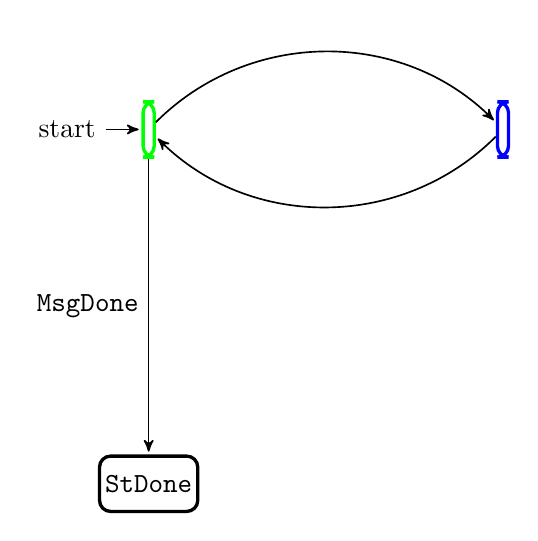
\begin{tikzpicture}[->,>=stealth',shorten >=1pt,auto,node distance=4.5cm, semithick]
  \tikzstyle{every state}=[fill=red,draw=none,text=white]
  \node[state, green, initial]        (Client)  {\Client};
  \node[state, blue, right of=Client] (Server)  {\Server};
  \node[state, below of=Client]       (Done)    {\StDone};

  \draw (Client) edge[above, bend left=45] node{\MsgKeepAlive}         (Server);
  \draw (Server) edge[below, bend left=45] node{\MsgKeepAliveResponse} (Client);
  \draw (Client) edge[left]                node{\MsgDone}              (Done);
\end{tikzpicture}

\begin{description}
\item [\MsgKeepAlive{} $cookie$]
  Keep alive message.  The $cookie$ value is a \texttt{Word16} value which allows to
  match requests with responses.  It is a protocol error if the cookie received
  back with \MsgKeepAliveResponse{} does not match the value sent with
  \MsgKeepAlive{}.
\item [\MsgKeepAliveResponse{} $cookie$]
  Keep alive response message. 
\item [\MsgDone]
  Terminating message.
\end{description}

\subsection{CDDL encoding specification}
\lstinputlisting[style=cddl]{../../ouroboros-network/test-cddl/specs/keep-alive.cddl}

\section{Local Transaction Submission Mini Protocol}
\haddockref{Ouroboros.Network.Protocol.LocalTxSubmission.Type}{ouroboros-network/Ouroboros-Network-Protocol-LocalTxSubmission-Type\#t:LocalTxSubmission}
\label{local-tx-submission-protocol}
\subsection{Description}
The local transaction submission mini protocol is used by local clients,
for example wallets or CLI tools, to submit transactions to a local node.
The protocol is {\bf not} used to forward transactions from one core node to an other.
The protocol for the transfer of transactions between full nodes
is described in Section \ref{tx-submission-protocol}.

The protocol follows a simple request-response pattern:
\begin{enumerate}
\item The client sends a request with a single transaction.
\item The Server either accepts the transaction (returning a confirmation) or rejects it (returning the
  reason).
\end{enumerate}
Note, that the local transaction submission protocol is a push based protocol where the client
creates a workload for the server.
This is acceptable because is protocol is only for use between a node and local client.
\newcommand{\SubmitTx}{\trans{SubmitTx}}
\newcommand{\AcceptTx}{\trans{AcceptTx}}
\newcommand{\RejectTx}{\trans{RejectTx}}
\subsection{State machine}

\begin{tabular}{|l|l|}
  \hline
  \multicolumn{2}{|c|}{Agency} \\ \hline
  Client has Agency & \StIdle \\ \hline
  Server has Agency & \StBusy \\  \hline
\end{tabular}

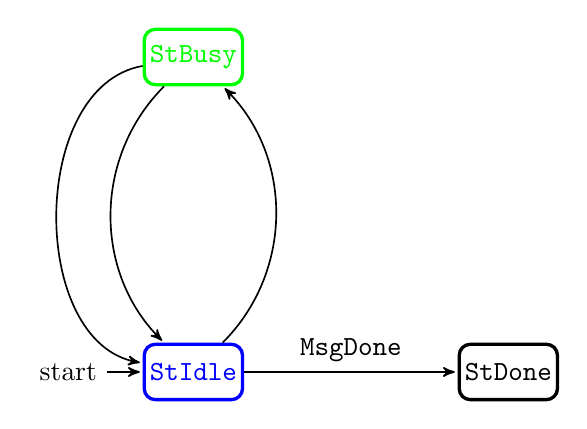
\begin{tikzpicture}[->,>=stealth',shorten >=1pt,auto,node distance=4cm, semithick]
  \tikzstyle{every state}=[fill=red,draw=none,text=white]
  \node[state, blue, initial]                                     (Idle)     {\StIdle};
  \node[state, right of=Idle]                                     (Done)     {\StDone};
  \node[state, green, above of=Idle]                              (Busy)     {\StBusy};

  \draw (Idle)         edge[]                          node{\MsgDone}           (Done);
  \draw (Idle)         edge[right, bend right=45]      node{\SubmitTx}          (Busy);
  \draw (Busy)         edge[left, bend right=45]       node[below = 3mm]{\AcceptTx}          (Idle);
  \draw (Busy)         edge[left, bend right=80]       node[above = 3mm]{\RejectTx}          (Idle);
\end{tikzpicture}

Messages of the protocol:
\begin{description}
\item [\SubmitTx{} {\boldmath $(t)$}]
      The client submits a transaction.
\item [\AcceptTx]
      The server accepts the transaction.
\item [\RejectTx{} {\boldmath $(reason)$}]
      The server rejects the transactions and replies with the $reason$.
\item [\MsgDone]
      The client terminates the mini protocol.
\end{description}

\section{Local State Query Mini Protocol}
\label{local-state-query-protocol}
\haddockref{Ouroboros.Network.Protocol.LocalStateQuery.Type}{ouroboros-network/Ouroboros-Network-Protocol-LocalStateQuery-Type\#t:LocalStateQuery}
\newcommand{\StAcquiring}{\state{Acquiring}}
\newcommand{\StAcquired}{\state{Acquired}}
\newcommand{\StQuerying}{\state{Querying}}
\newcommand{\MsgAcquire}{\trans{MsgAcquire}}
\newcommand{\MsgAcquired}{\trans{MsgAcquired}}
\newcommand{\MsgFailure}{\trans{MsgFailure}}
\newcommand{\MsgQuery}{\trans{MsgQuery}}
\newcommand{\MsgResult}{\trans{MsgResult}}
\newcommand{\MsgRelease}{\trans{MsgRelease}}
\newcommand{\MsgReAcquire}{\trans{MsgReAcquire}}

\subsection{Description}
Local State Query mini-protocol allows to query the consensus \/ ledger state.
This mini protocol is part of the Node-to-Client protocol, hence it is only
used by local (and thus trusted) clients.  Possible queries depend on the era
(Byron, Shelly, etc) and are not specified in this document.  The protocol
specifies basic operations like acquiring / releaseing the consensus \/ ledger
state which is done by the server, or running queries against the acquired
ledger state.

\subsection{State machine}

\begin{figure}[h]
\begin{tabular}{|l|l|}
  \hline
  \multicolumn{2}{|c|}{Agency} \\ \hline
  Server has Agency & \StIdle{}, \StAcquired{} \\ \hline
  Client has Agency & \StAcquiring{}, \StQuerying{} \\ \hline
\end{tabular}
\end{figure}

\begin{figure}[h]
\begin{tikzpicture}[->,=>stealth',shorten >=1pt,auto,node distance=4cm,semithick]
  \tikzstyle{every state}=[fill=red,draw,none,text=white]
  \node[state, green, initial] (Idle) {\StIdle};
  \node[state, blue, right of=Idle] (Acquiring) {\StAcquiring};
  \node[state, green, right of=Acquiring] (Acquired) {\StAcquired};
  \node[state, blue, right of=Acquired] (Querying) {\StQuerying};

  \draw (Idle)      edge[bend left=45] node{\MsgAcquire}   (Acquiring);
  \draw (Acquiring) edge[bend left=45] node{\MsgFailure}   (Idle);
  \draw (Acquiring) edge[bend left=45] node{\MsgAcquired}  (Acquired);
  \draw (Acquired)  edge[bend left=45] node{\MsgReAcquire} (Acquiring);
  \draw (Acquired)  edge[bend left=45] node{\MsgQuery}     (Querying);
  \draw (Querying)  edge[bend left=45] node{\MsgResult}    (Acquired);
\end{tikzpicture}
\end{figure}

\begin{figure}[h]
\begin{tabular}{|l|l|l|l|}
  \hline
  \multicolumn{4}{|c|}{Transition table} \\ \hline
  from state          & message             & parameters          & to state \\ \hline\hline
  \StIdle             & \MsgAcquire         & $Maybe\ point$      & \StAcquiring \\\hline
  \StAcquiring        & \MsgFailure         & $AcquireFailure$    & \StIdle      \\\hline
  \StAcquiring        & \MsgAcquired        &                     & \StAcquired  \\\hline
  \StAcquired         & \MsgReAcquire       & $Maybe\ point$      & \StAcquiring \\\hline
  \StAcquired         & \MsgQuery           & $query$             & \StQuerying  \\\hline
  \StQuerying         & \MsgResult          & $result$            & \StAcquired  \\\hline
\end{tabular}
\end{figure}

where $AcquireFailure$ is either $AcquireFailurePointTooOld$ or
$AcquireFailurePointNotOnChain$.

\subsection{CDDL encoding specification}
\lstinputlisting[style=cddl]{../../ouroboros-network/test-cddl/specs/local-state-query.cddl}
See appendix \ref{cddl-common} for common definitions.

\section{Pipelining of Mini Protocols}
\label{pipelining}
Protocol pipelining is a technique that improves the performance of some protocols.
The underlying idea is that a client, which wants to perform several requests,
just transmits those requests in sequence without blocking and waiting for the reply from the server.
In the reference implementation, pipelining is used by the clients of all mini protocol except Chain-Sync.
Those mini protocols follow a request-response pattern that is amenable to pipelining such
that pipelining becomes a feature of the client implementation that does not require any
modifications of the server implementation.

As an example, let's consider the Block-Fetch mini protocol.
When a client follows the protocol and sends a sequence of \MsgRequestRange~messages to the server
the data stream from the client to the server will only consist of \MsgRequestRange~messages
(and a final \MsgClientDone~message) and no other message types.
The server can simply follow the state machine of the protocol and process the messages in turn,
regardless whether the client uses pipelining or not.
The MUX/DEMUX layer (Section~\ref{multiplexing-section}) guarantees
that messages of the same mini protocol are delivered in transmission order,
and therefore the client can determine which response belongs to which request.

The MUX/DEMUX layer also provides a fixed size buffer between the egress of DEMUX and the ingress
of mini protocol thread.
The size of this buffer is a protocol parameter that determines how many messages
a client can send before waiting for a reply from the server (see Section~\ref{mux-flow-control}).
The protocol requires that a client must never cause a overrun of these buffers on a server node.
If a message arrives at the server that would cause the buffer to overrun,
the server treats this case as a protocol violation of the peer
(and closes the connection to the peer).
\hide{
The buffer sizes are listed in Table~\ref{bla} in Section~\ref{blub}.
}

\section{Node-to-node protocol}
\haddockref{Ouroboros.Network.NodeToNode}{ouroboros-network/Ouroboros-Network-NodeToNode}\newline
\haddockref{Ouroboros.Network.NodeToNode.Version}{ouroboros-network/Ouroboros-Network-NodeToNode-Version}\newline

The node-to-node protocol consists of the following protocols:

\begin{itemize}
  \item chain synchronisation mini-protocol for headers
  \item block fetch mini-protocol
  \item transaction submission mini-protocol (from $NodeToNodeV\_6$ the version
        2 is used)
  \item keep alive mini-protocol (from $NodeToNodeV\_3$)
\end{itemize}

Currently there are the following versions of the node-to-node protocol:
\begin{figure}[h]
\begin{tabular}{l|l}
  version         & description \\\hline\hline
  $NodeToNodeV\_1$ & initial version \\\hline
  $NodeToNodeV\_2$ & block size hints \\\hline
  $NodeToNodeV\_3$ & introduction of keep-alive mini-protocol \\\hline
  $NodeToNodeV\_4$ & introduction of diffusion mode in handshake mini-protocol \\\hline
  $NodeToNodeV\_5$ & \\\hline
  $NodeToNodeV\_6$ & transaction submission version 2 \\\hline
\end{tabular}
\end{figure}

\section{Node-to-client protocol}
\haddockref{Ouroboros.Network.NodeToClient}{ouroboros-network/Ouroboros-Network-NodeToClient}\newline
\haddockref{Ouroboros.Network.NodeToClient.Version}{ouroboros-network/Ouroboros-Network-NodeToClient-Version}\newline

The node-to-client protocol consists of the following protocols:
\begin{itemize}
  \item chains synchronisation mini-protocols for blocks
  \item local transaction submission mini-protocol
  \item local state query mini-protocol (from version $NodeToClient\_2$)
\end{itemize}

Currenty there are the following version of the node-to-client protocol:
\begin{figure}[h]
\begin{tabular}{l|l}
  version & description \\\hline\hline
  $NodeToClientV\_1$ & initial version\\\hline
  $NodeToClientV\_2$ & added local-query mini-protocol\\\hline
  $NodeToClientV\_3$ & \\\hline
  $NodeToClientV\_4$ & new queries added to local state query mini-protocol\\\hline
  $NodeToClientV\_5$ & allegra \\\hline
  $NodeToClientV\_6$ & mary \\\hline
  $NodeToClientV\_7$ & new queries added to local state query mini-protocol\\\hline
  $NodeToClientV\_8$ & codec changed for local state query mini-protocol\\\hline
\end{tabular}
\end{figure}



% \wip{
  % \section{DeltaQ Mini Protocol}

  % WIP : Explain DeltaQ measurement back pressure and how we deal with slow
  % connection.  See Section % ~\ref{deltaq-discussion}.  The DeltaQ mini
  % protocol does not transmit is own messages.  Instead it relies on the time
  % stamps that the multiplexing layer (Section~\ref{multiplexing-section}) adds
  % to the messages of other mini protocols.
% }


% TODO:
% Discussion of interaction between inbound protocol governor and connection
% manager when a new outbound connection is requested.

% TODO:
% I realised that it would be nicer to structure the spec a bit differently.
% First describe each transition in general terms, without referring to the
% implementation, and in a subsequent section introduce implementation details.

\chapter{Connection Manager State Machine Specification}
\label{chapter:connection-manager}

\tikzstyle{decision} =
  [ diamond
  , fill=DarkSeaGreen1
  , text width=4.5em
  , text badly centered
  , node distance=3cm
  , inner sep=0pt
  ]
\tikzstyle{outbound_state} =
  [ rectangle
  , rounded corners
  , fill=DodgerBlue1
  , minimum height=2em
  ]
\tikzstyle{inbound_outbound_state} =
  [ rectangle
  , rounded corners
  , fill=HotPink3
  , minimum height=2em
  ]
\tikzstyle{inbound_state} =
  [ rectangle
  , rounded corners
  , fill=DarkOliveGreen3
  , minimum height=2em
  ]
\tikzstyle{impossible_outbound_state} =
  [ rectangle
  , rounded corners
  , fill=LightBlue2
  , rounded corners
  , minimum height=2em
  ]
\tikzstyle{line} =
  [ draw
  , -latex'
  ]
\tikzstyle{error} =
  [ rectangle
  , rounded corners
  , fill=red!255!blue!20
  , minimum height=2em
  ]
\tikzstyle{requestOutboundArr}      = [ color = DodgerBlue1 ]
\tikzstyle{registerInboundArr}      = [ color = HotPink3 ]
\tikzstyle{promotedToWarmRemoteArr} = [ color = DarkOliveGreen3 ]
\tikzstyle{demotedToColdRemoteArr}  = [ color = Orange2 ]
\tikzstyle{unregisterOutboundArr}   = [ color = Turquoise ]
\tikzstyle{unregisterInboundArr}    = [ color = DarkOrchid2 ]

\def\TCP{\textsf{TCP}}
\def\ipvfour{\textsf{ipv4}}
\def\ipvsix{\textsf{ipv6}}

% Connection manager's states
\def\InitialState{\textbullet}
\def\FinalState{\textbullet}
\def\ReservedOutboundState{\texttt{ReservedOutboundState}}
\def\UnnegotiatedStateOut{\texttt{UnnegotiatedState Outbound}}
\def\UnnegotiatedStateIn{\texttt{UnnegotiatedState Inbound}}
\def\UnnegotiatedStateAny{\texttt{UnnegotiatedState prov}}
\def\OutboundStateUni{\texttt{OutboundState Unidirectional}}
\def\OutboundStateDup{\texttt{OutboundState Duplex}}
\def\OutboundStateDupTau{\texttt{OutboundState\textsuperscript{$\tau$} Duplex}}
\def\OutboundStateDupP{\texttt{OutboundState\phantom{\textsuperscript{$\tau$}} Duplex}}
\def\OutboundStateUniTau{\texttt{OutboundState\textsuperscript{$\tau$} Unidirectional}}
\def\OutboundStateAny{\texttt{OutboundState dataFlow}}
\def\OutboundStateAnyTau{\texttt{OutboundState\textsuperscript{$\tau$} dataFlow}}
\def\DuplexState{\texttt{DuplexState}}
\def\InboundStateUni{\texttt{InboundState Unidirectional}}
\def\InboundStateDup{\texttt{InboundState Duplex}}
\def\InboundStateAny{\texttt{InboundState dataFlow}}
\def\WaitRemoteIdle{\texttt{WaitRemoteIdleState}}
\def\InboundIdleStateUni{\texttt{InboundIdleState\textsuperscript{$\tau$} Unidirectional}}
\def\InboundIdleStateDup{\texttt{InboundIdleState\textsuperscript{$\tau$} Duplex}}
\def\InboundIdleStateAny{\texttt{InboundIdleState\textsuperscript{$\tau$} dataFlow}}
\def\OutboundIdleStateUni{\texttt{OutboundIdleState\textsuperscript{$\tau$} Unidirectional}}
\def\OutboundIdleStateDup{\texttt{OutboundIdleState\textsuperscript{$\tau$} Duplex}}
\def\OutboundIdleStateAny{\texttt{OutboundIdleState\textsuperscript{$\tau$} dataFlow}}
\def\TerminatingState{\texttt{TerminatingState\textsuperscript{$\tau$}}}
\def\TerminatedState{\texttt{TerminatedState}}

% Connection manager's ransitions
\def\Reserve{\textsf{Reserve}}
\def\Connected{\textsf{Connected}}
\def\Accepted{\textsf{Accepted}}
\def\Overwritten{\textsf{Overwritten}}
\def\NegotiatedUniOut{\textsf{Negotiated}\textsuperscript{\textsf{Unidirectional}}\textsubscript{\textsf{Outbound}}}
\def\NegotiatedDupOut{\textsf{Negotiated}\textsuperscript{\textsf{Duplex}}\textsubscript{\textsf{Outbound}}}
\def\NegotiatedUniIn{\textsf{Negotiated}\textsuperscript{\textsf{Unidirectional}}\textsubscript{\textsf{Inbound}}}
\def\NegotiatedDupIn{\textsf{Negotiated}\textsuperscript{\textsf{Duplex}}\textsubscript{\textsf{Inbound}}}
\def\NegotiatedAnyIn{\textsf{Negotiated}\textsuperscript{\textsf{dataFlow}}\textsubscript{\textsf{Inbound}}}
\def\PromotedToWarmDupLoc{\textsf{PromotedToWarm}\textsuperscript{\textsf{Duplex}}\textsubscript{\textsf{Local}}}
\def\PromotedToWarmDupRem{\textsf{PromotedToWarm}\textsuperscript{\textsf{Duplex}}\textsubscript{\textsf{Remote}}}
\def\PromotedToWarmAnyRem{\textsf{PromotedToWarm}\textsuperscript{\textsf{dataFlow}}\textsubscript{\textsf{Remote}}}
\def\DemotedToColdDupLoc{\textsf{DemotedToCold}\textsuperscript{\textsf{Duplex}}\textsubscript{\textsf{Local}}}
\def\DemotedToColdAnyLoc{\textsf{DemotedToCold}\textsuperscript{\textsf{dataFlow}}\textsubscript{\textsf{Local}}}
\def\DemotedToColdDupRem{\textsf{DemotedToCold}\textsuperscript{\textsf{Duplex}}\textsubscript{\textsf{Remote}}}
\def\TimeoutExpired{\textsf{TimeoutExpired}}
\def\DemotedToColdAnyRem{\textsf{DemotedToCold}\textsuperscript{\textsf{dataFlow}}\textsubscript{\textsf{Remote}}}
\def\DemotedToColdUniLoc{\textsf{DemotedToCold}\textsuperscript{\textsf{Unidirectional}}\textsubscript{\textsf{Local}}}
\def\DemotedToColdUniRem{\textsf{DemotedToCold}\textsuperscript{\textsf{Unidirectional}}\textsubscript{\textsf{Remote}}}
\def\Restart{\textsf{Restart}}
\def\Prune{\textsf{Prune}}
\def\CommitDupRem{\textsf{Commit}\textsuperscript{\textsf{Duplex}}\textsubscript{\textsf{Remote}}}
\def\CommitUniRem{\textsf{Commit}\textsuperscript{\textsf{Unidirectional}}\textsubscript{\textsf{Remote}}}
\def\CommitAnyRem{\textsf{Commit}\textsuperscript{\textsf{dataFlow}}\textsubscript{\textsf{Remote}}}
\def\AwakeDupRem{\textsf{Awake}\textsuperscript{\textsf{Duplex}}\textsubscript{\textsf{Remote}}}
\def\AwakeUniRem{\textsf{Awake}\textsuperscript{\textsf{Unidirectional}}\textsubscript{\textsf{Remote}}}
\def\AwakeAnyRem{\textsf{Awake}\textsuperscript{\textsf{dataFlow}}\textsubscript{\textsf{Remote}}}
\def\AwakeDupLoc{\textsf{Awake}\textsuperscript{\textsf{Duplex}}\textsubscript{\textsf{Local}}}
\def\CommitAnyLoc{\textsf{Commit}\textsuperscript{\textsf{dataFlow}}\textsubscript{\textsf{Local}}}
\def\CommitDupLoc{\textsf{Commit}\textsuperscript{\textsf{Duplex}}\textsubscript{\textsf{Local}}}
\def\CommitUniLoc{\textsf{Commit}\textsuperscript{\textsf{Unidirectional}}\textsubscript{\textsf{Local}}}
\def\Terminate{\textsf{Terminate}}
\def\Timeout{\textsf{Timeout}}

% Inbound governor states
\def\RemoteEstablished{\textsf{RemoteEstablished}}
\def\RemoteIdle{\textsf{RemoteIdle}\textsuperscript{$\tau$}}
\def\RemoteCold{\textsf{RemoteCold}}

% Inbound governor transitions
\def\NewInboundConnection{\textsf{NewConnection Inbound}}
\def\NewOutboundConnection{\textsf{NewConnection Outbound}}
\def\NewConnectionAny{\textsf{NewConnection provenance}}
\def\AwakeRemote{\textsf{AwakeRemote}}
\def\RemoteToCold{\textsf{RemoteToCold}}
\def\CommitRemote{\textsf{CommitRemote}}

% Peer states
\def\cold{\textit{cold}}
\def\warm{\textit{warm}}
\def\hot{\textit{hot}}
\def\established{\textit{established}}

% Protocol names
\def\keepAlive{\textsf{keep-alive}}
\def\tipSample{\textsf{tip-sample}}

% Component names
\def\ptopgov{\textit{p2p governor}}
\def\mux{\textit{mux}}
\def\inbgov{\textit{inbound protocol governor}}
\def\Inbgov{\textit{Inbound protocol governor}}
\def\connmngr{\textit{connection manager}}
\def\Connmngr{\textit{Connection manager}}
\def\True{\texttt{True}}
\def\False{\texttt{False}}

% Utils

% TODO notes for the implementation
\newcommand{\todoimpl}[1]{\todo[backgroundcolor=red,linecolor=red]{#1}}
\newenvironment{detail}
  {
    \begin{center}
    \begin{minipage}{0.9\textwidth}
      \begin{shaded}
      \small
      \noindent Implementation detail
      \vspace{0.3em}
      \newline
      \itshape
  }
  {
  \end{shaded}
  \end{minipage}
  \end{center}
  \vspace{1em}
  }

\section{Introduction}

As described in the \href{https://hydra.iohk.io/build/5866649/download/1/network-design.pdf}{Network Design} document, the goal is to transition to a more
decentralized network. To make that happen, a plan was designed to come up with a P2P
network that is capable to achieve desired network properties. One key component of
such design is the \ptopgov{}, which is responsible for managing the \cold{}/\warm{}/\hot{}
peer selection and managing the churn of these groups, and adjusting the targets in order for
the network to reach the desired properties. However, having \warm{} and \hot{} peers implies
establishing a bearer connection; \hot{} peers need to run several mini-protocols, and each
mini-protocol runs 2 instances (client and server). Which means that with a large enough
warm/hot peer target, there's going to be a lot of resource waste when it comes to file
descriptor usage. There's also the problem of firewalls, where it matters who tries to
start a communication with whom (if it's the client or the server).

Knowing this, it would be good to make the most of each connection and, in order to do so the
\Connmngr{} was designed.

\section{Components}

Figure \ref{tik:components} illustrates the 3 main components of the decentralization
process, from the perspective of a local node. In the \texttt{Outbound} side, the
\ptopgov{}, as said previously, takes care of all connection initiation (outbound
connections) and decides which mini-protocols to run (\established{}, \warm{} or \hot{}).
In the \texttt{Inbound} side, the \texttt{Server} is just a simple loop, responsible for accepting incoming
connections; and the \texttt{Inbound Protocol Governor} role is to detect if its local peer was
added as a \warm{}/\hot{} peer in some other remote node, starting/restarting the required
mini-protocols. Another role of the \texttt{Inbound Protocol Governor} is to setup timers in
some cases, e.g. if the remote end opened a connection, and did not sent any message, the
\texttt{Inbound Protocol Governor} will timeout after some time and close the connection.
The arrows in Figure \ref{tik:components} represent dependencies between components:
server accepts a connection which is then given to \Connmngr{}. \Connmngr{} exposes methods to update its state,
whenever the \texttt{Inbound Protocol Governor} notices that the connection was used
(could be used due to \warm{}\\hot{} transitions).

\begin{figure}[h]
  \footnotesize
  \def\xa{-2.0}
  \def\xb{2.0}
  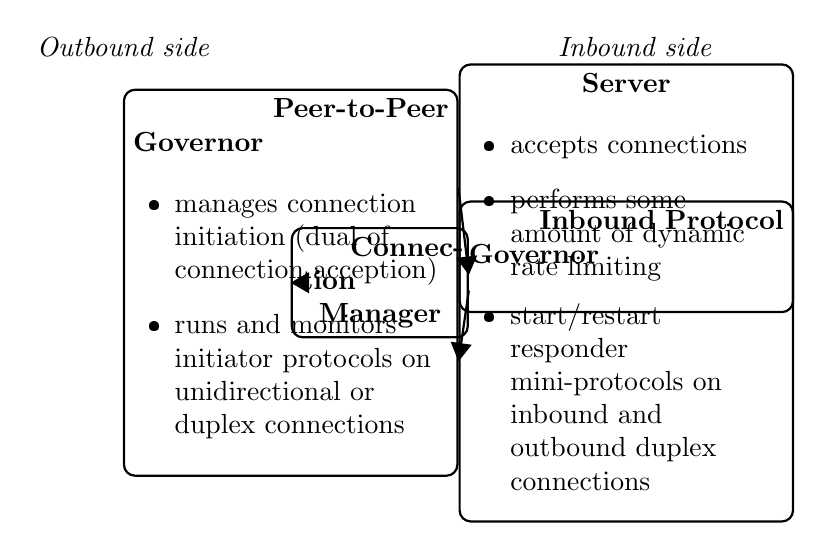
\begin{tikzpicture}
    \node at (-3.25, 0)  {\textit{Outbound side}};
    \node at ( 3.25, 0)  {\textit{Inbound side}};

    \node[rounded corners, rectangle, draw, minimum height=3cm,anchor=east, text width=4cm] (p2p_governor) at (\xa, -3)
     {
       \hfil\textbf{Peer-to-Peer Governor}\hfil\\
       \setlength{\leftmargini}{15pt}
       \begin{itemize}
        \item manages connection initiation (dual of connection acception)
        \item runs and monitors initiator protocols on unidirectional or duplex connections
      \end{itemize}
      \vspace{5pt}
      };

    \node[rounded corners, rectangle, draw, anchor=west, text width=4cm] (server) at (\xb, -1.80)
      {
        \hfill{\textbf{Server}}\hfill
        \vspace{0.2em}
        \setlength{\leftmargini}{15pt}
        \begin{itemize}
          \item accepts connections
          \item performs some amount of dynamic rate limiting
        \end{itemize}
        \vspace{5pt}
      };

    \node[rounded corners, rectangle, draw, anchor=west, text width=4cm] (inbound_governor) at (\xb, -4)
      {
        \hfill{\textbf{Inbound Protocol Governor}}\hfill
        \vspace{0.2em}
        \setlength{\leftmargini}{15pt}
        \begin{itemize}
          \item start/restart responder mini-protocols on inbound and
            outbound duplex connections
        \end{itemize}
        \vspace{5pt}
      };

    \node[rounded corners, rectangle, draw, minimum height=1cm, text width=2cm] (connection_manager) at (0, -3)
      {
        \hfil\textbf{Connection}\hfil\\
        \hfil\textbf{Manager}\hfil
      };

    \draw[<-] (p2p_governor)           -- (connection_manager);
    \draw[->] (server.west)            -- (connection_manager.5);
    \draw[->] (connection_manager.355) -- (inbound_governor.west);
  \end{tikzpicture}
  \caption{3 main components}
  \label{tik:components}
\end{figure}

One simple illustration of how these 3 components interact together:

\begin{itemize}
    \item Server accepts a connection;
    \item Server registers that connection to the connection manager (which puts the
      connection in \UnnegotiatedStateIn{});
    \item Assuming the handshake was successful, the connection is put in
      \InboundIdleStateDup{};
    \item The remote end transitions the local node to warm (using the connection) within expected timeout;
    \item IPG (Inbound Protocol Governor) notifies the \Connmngr{} about this state
      change, via \texttt{promotedToWarmRemote}. Now the connection is
      in \InboundStateDup{};
    \item \Connmngr{} is asked for an outbound connection to that peer (by the \ptopgov{}), it notices
      that it already has a connection with that peer in \InboundStateDup{}, so it gives
      that connection to \ptopgov{} and updates its state to \DuplexState{}.
\end{itemize}

You can find more information about the possible different connection states in section
\ref{sec:connection-state}.

\begin{figure}
    \centering
    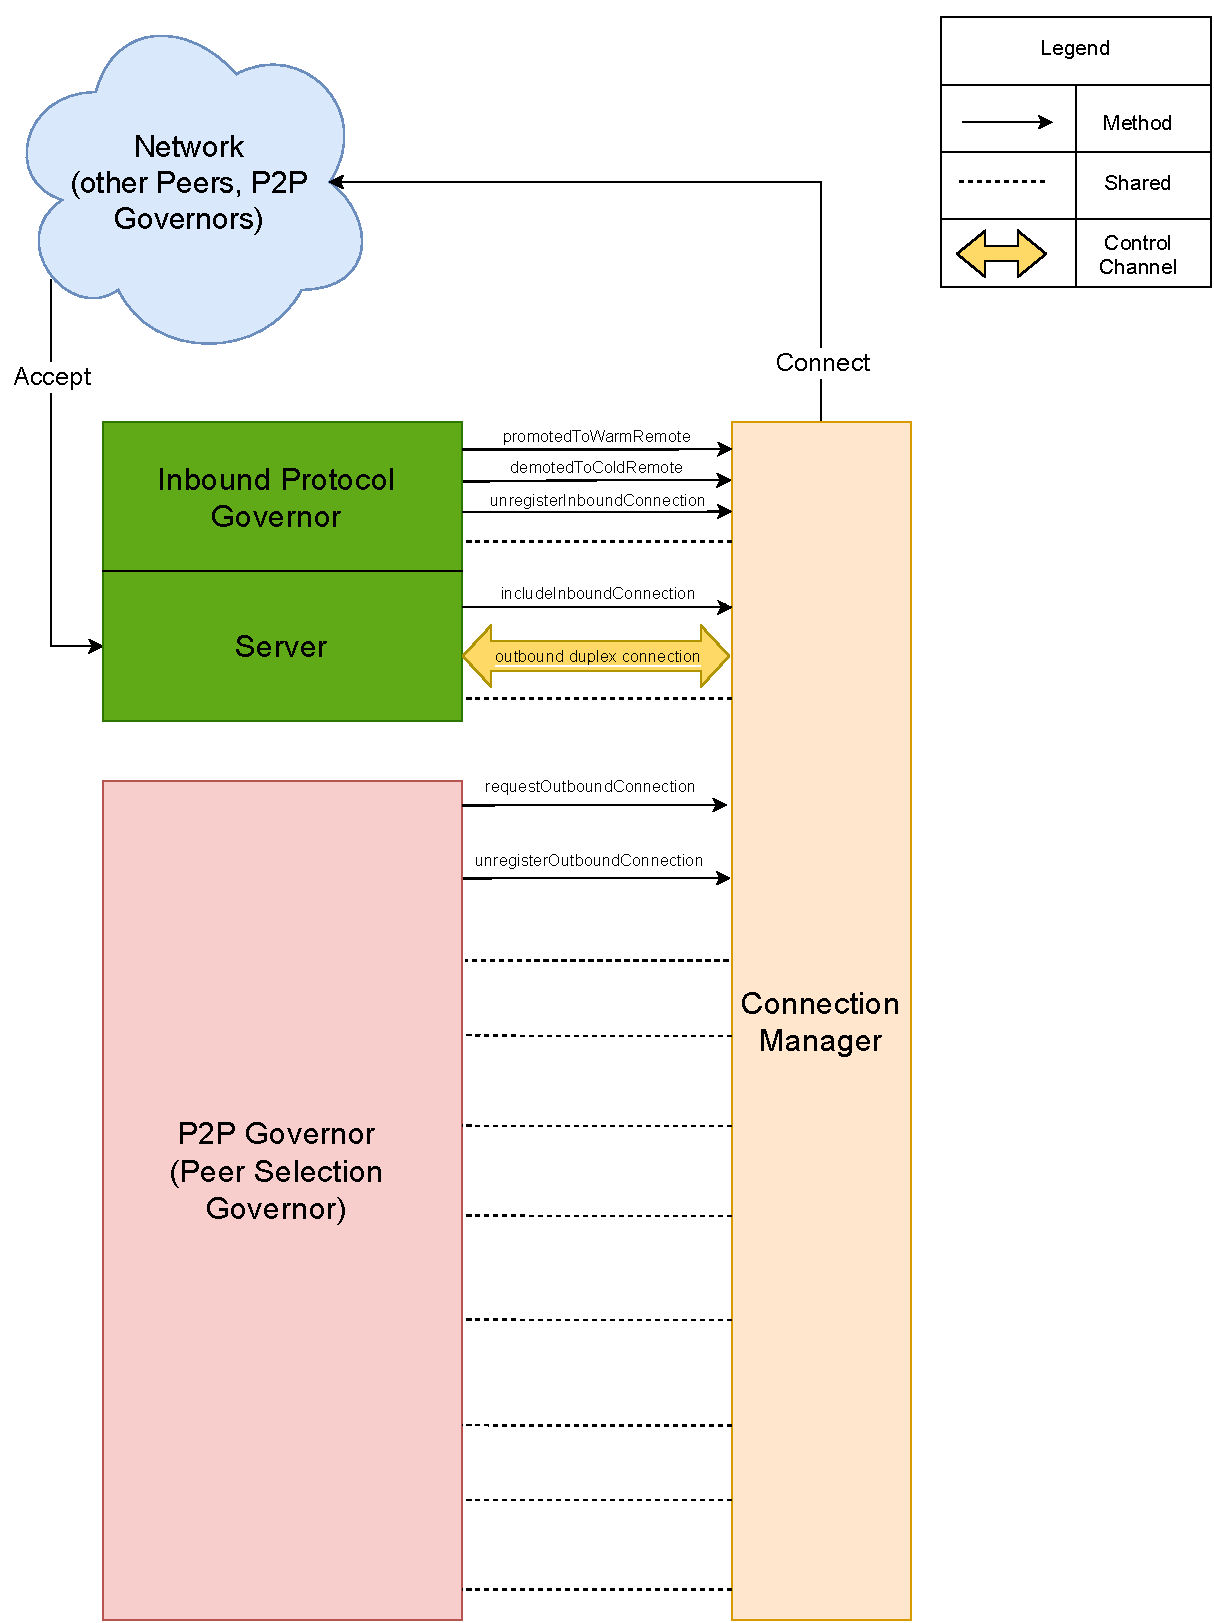
\includegraphics[width=\linewidth]{figure/ConnectionManagerInteractions.pdf}
    \caption{High-level architecture of how the 3 components interact}
    \label{fig:high-level-arch}
\end{figure}

Figure \ref{fig:high-level-arch} shows the high-level architecture of how the 3 components mentioned interact
with each other. A single \Connmngr{} is shared between the \emph{Server} and \ptopgov{},
where, in case of an \emph{Outbound Duplex} connection is negotiated, the \emph{Server} is
notified via a control channel. Although in this document we will use Server and IPG
interchangeably, it is worth to keep them separate concepts for possible future
developments.

\section{Connection Manager}

\subsection{Overview}

\Connmngr{} is a lower-level component responsible for managing connections and its
resources. Its responsibilities consist of:

\begin{itemize}
    \item Tracking each connection, in order to keep an eye on the bounded resources;
    \item Starting new connections, negotiating if the connection should be
      \emph{full-duplex} or \emph{half-duplex}, through the \emph{Connection Handler};
    \item Be aware of \warm{}/\hot{} transitions, in order to try and reuse already established
      connections;
    \item Negotiating which direction, which mini-protocol is going to run
      (Client $\rightarrow$ Server, Server$\rightarrow$Client, or both);
    \item Taking care of a particularity of TCP connection termination (lingering
      connections).
\end{itemize}

The \Connmngr{} creates and records accepted connections and keeps track of their state
as negotiations, for the connection and start/stop mini-protocols, are made. There's an
\emph{internal state machine} that helps the \Connmngr{} keep track of the state of each
connection, and help it make decisions when it comes to resource management and
connection reusing.

The \emph{Connection Handler} drives through handshake negotiation and starts the multiplexer. The
outcome of the handshake negotiation is:

\begin{itemize}
    \item the negotiated version of the protocol
    \item negotiated parameters, which includes the mode in which the connection will be
      run (\texttt{InitiatorOnlyMode}, \texttt{ResponderOnlyMode},\\
      \texttt{InitiatorAndResponderMode} - the first two are \emph{half-duplex}, the last
      one is \emph{full-duplex} mode)
    \item Handshake might error
\end{itemize}

\begin{figure}
    \centering
    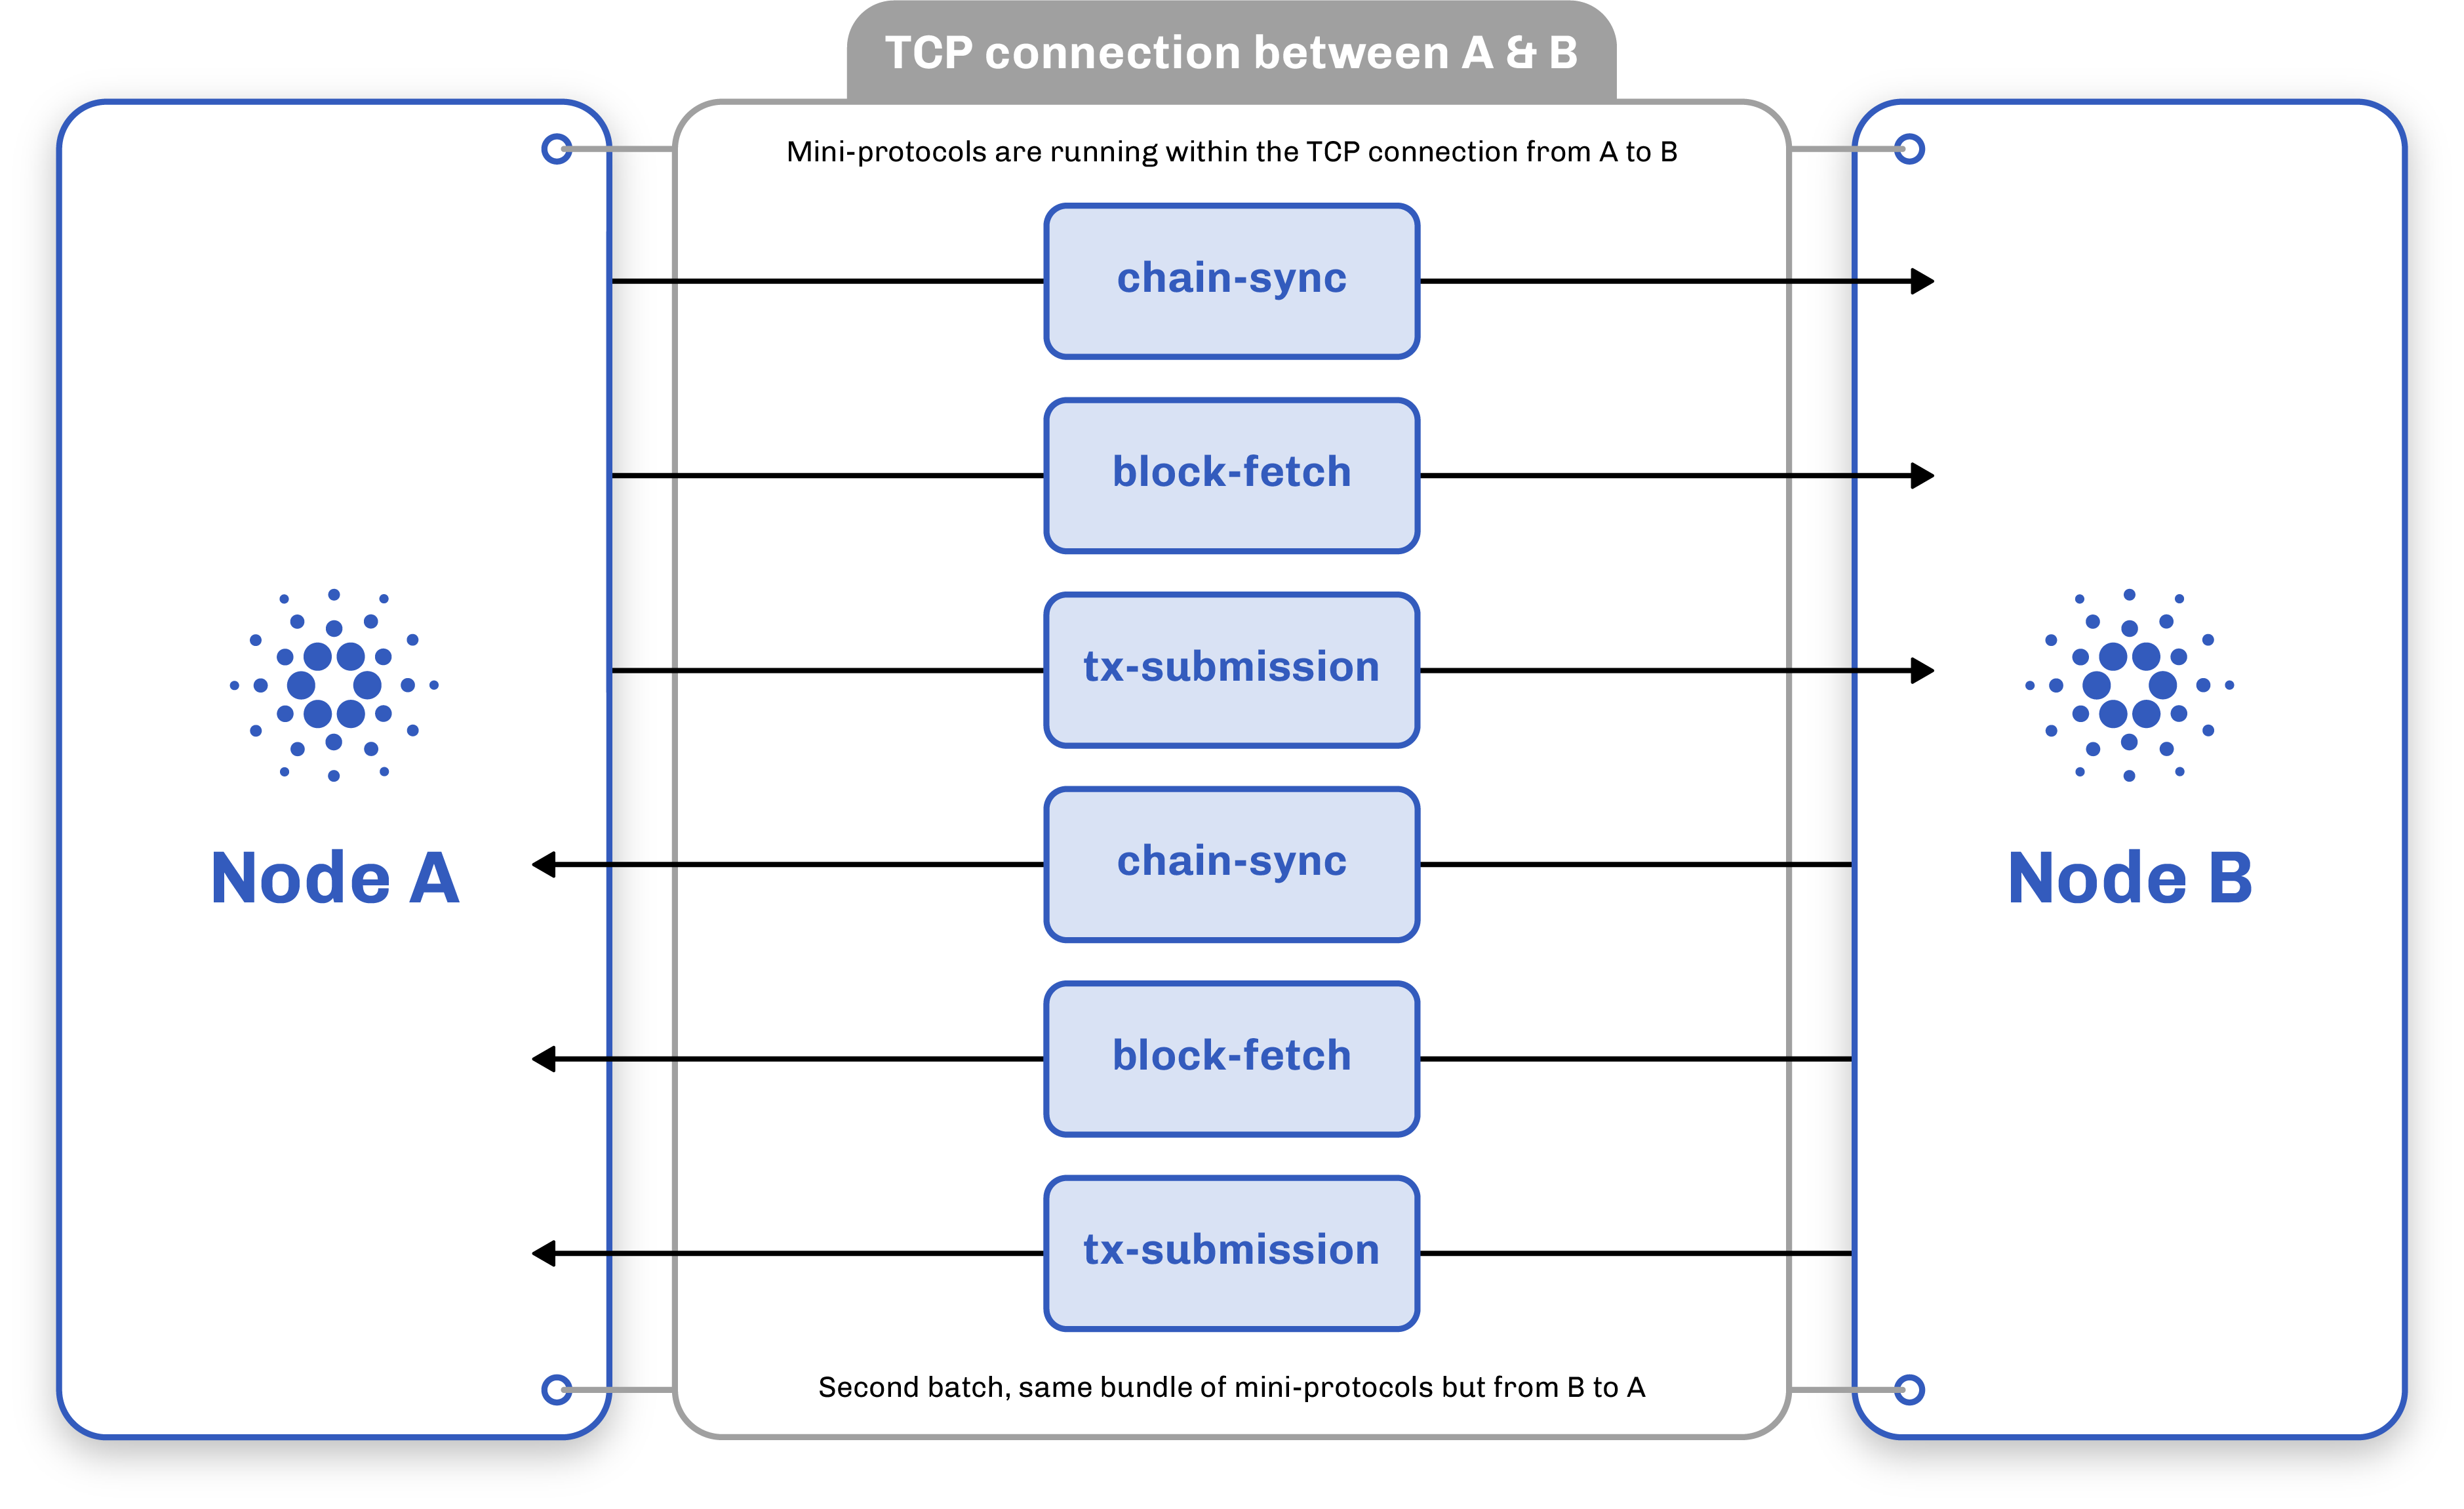
\includegraphics[width=\linewidth]{figure/node-to-node-ipc.png}
    \caption{Duplex connection running severall mini-protocols}
    \label{fig:protocol-diagram}
\end{figure}

The \emph{Connection Handler} notifies the \Connmngr{} about the result of a negotiation, which
triggers a state transition. If we can run the connection in full-duplex mode,
then it is possible to run the bundles of mini-protocols in both directions, and otherwise only in one direction.
So, Figure \ref{fig:protocol-diagram} shows $6$ mini protocols running, $3$ in each direction.
If we negotiated only a unidirectional connection, then we'd only be running $3$
(with the direction being based on which peer established the connection).

From the point of view of the \connmngr{}, it only
matters whether an \emph{unidirectional} or \emph{duplex} connection was negotiated.
Unidirectional connections, are the ones which run either the initiator or responder
side of mini-protocols, exclusively, while duplex connections can run either or
both initiator and responder protocols. Note that in the outbound direction (initiator side),
it is the \ptopgov{} responsibility to decide which set of mini-protocols:
\established{}, \warm{} or \hot{}, are running. On the inbound side (responder
mini-protocols), we have no choice but to run all of them.

The \connmngr{} should only be run in two \texttt{MuxMode}s:

\begin{itemize}
  \item \texttt{ResponderMode} or
  \item \texttt{InitiatorAndResponderMode}
\end{itemize}

\noindent, the \texttt{InitiatorMode} is not allowed, since that mode is reserved for
special leaf nodes in the network (such as the blockchain explorer, for example) and it doesn't make
sense to run a node-to-client client side.

The duplex mode: \texttt{InitiatorAndResponderMode} is useful for managing
connection with external nodes (\textit{node-to-node protocol}), while
\texttt{ResponderMode} is useful for running a server which responds to local
connections (server side of \textit{node-to-client protocol}).


\Connmngr{} can use at most one \ipvfour{} and at most one \ipvsix{}
address. It will bind to the correct address depending on the remote address
type (\ipvfour{}/\ipvsix{}).

In this specification we will often need to speak about two nodes communicating
via a \TCP{} connection.  We will often call them local and remote ends of the
connection or local \slash{} remote nodes; we will usually take the
perspective of the local node.


\subsection{Types} % Not sure about this naming

\Connmngr{} exposes two methods to register a connection:

\begin{lstlisting}
data Connected peerAddr handle handleError
  -- | We are connected and mux is running.
  = Connected    !(ConnectionId peerAddr) !handle

  -- | There was an error during handshake negotiation.
  | Disconnected !(ConnectionId peerAddr) !(Maybe handleError)

-- | Include outbound connection into 'ConnectionManager'.

--   This executes:
--
-- * \(Reserve\) to \(Negotiated^{*}_{Outbound}\) transitions
-- * \(PromotedToWarm^{Duplex}_{Local}\) transition
-- * \(Awake^{Duplex}_{Local}\) transition
requestOutboundConnection
  *'$\coloncolon$'* HasInitiator muxMode ~ True
  *'$\Rightarrow$'* ConnectionManager muxMode socket peerAddr handle handleError m
  *'$\rightarrow$'* peerAddr *'$\rightarrow$'* m (Connected peerAddr handle handleError)

-- | Include an inbound connection into 'ConnectionManager'.

--   This executes:
--
-- * \(Accepted\) \/ \(Overwritten\) to \(Negotiated^{*}_{Inbound}\) transitions
includeInboundConnection
  *'$\coloncolon$'* HasResponder muxMode ~ True
  *'$\Rightarrow$'* ConnectionManager muxMode socket peerAddr handle handleError m
  *'$\rightarrow$'* socket *'$\rightarrow$'* peerAddr *'$\rightarrow$'* m (Connected peerAddr handle handleError)
\end{lstlisting}

The first one asks the \connmngr{} to either connect to an outbound peer or, if
possible, reuse a duplex connection. The other one allows to register an
inbound connection, which was \texttt{accepted}. Both methods are blocking
operations and return either an error (handshake negotiation error or
a multiplexer error) or a handle to a \textit{negotiated} connection.

Other methods which are discussed in this specification:

\begin{lstlisting}
-- | Custom either type for result of various methods.
data OperationResult a
    = UnsupportedState !InState
    | OperationSuccess a

-- | Enumeration of states, used for reporting; constructors elided from this
-- specification.
data InState

-- | Unregister an outbound connection.
--
--   This executes:
--
-- * \(DemotedToCold^{*}_{Local}\) transitions
unregisterOutboundConnection
  *'$\coloncolon$'* HasInitiator muxMode ~ True
  *'$\Rightarrow$'* ConnectionManager muxMode socket peerAddr handle handleError m
  *'$\rightarrow$'* peerAddr *'$\rightarrow$'* m (OperationResult ())

-- | Notify the 'ConnectionManager' that a remote end promoted us to a
-- /warm peer/.
--
-- This executes:
--
-- * \(PromotedToWarm^{Duplex}_{Remote}\) transition,
-- * \(Awake^{*}_{Remote}\) transition.
promotedToWarmRemote
  *'$\coloncolon$'* HasInitiator muxMode ~ True
  *'$\Rightarrow$'* ConnectionManager muxMode socket peerAddr handle handleError m
  *'$\rightarrow$'* peerAddr *'$\rightarrow$'* m (OperationResult InState)

-- | Notify the 'ConnectionManager' that a remote end demoted us to a /cold
-- peer/.
--
-- This executes:
--
-- * \(DemotedToCold^{*}_{Remote}\) transition.
demotedToColdRemote
  *'$\coloncolon$'* HasResponder muxMode ~ True
  *'$\Rightarrow$'* ConnectionManager muxMode socket peerAddr handle handleError m
  *'$\rightarrow$'* peerAddr -> m (OperationResult InState)

-- | Unregister outbound connection. Returns if the operation was successul.
--
-- This executes:
--
-- * \(Commit*{*}\) transition
-- * \(TimeoutExpired\) transition
unregisterInboundConnection
  *'$\coloncolon$'* HasResponder muxMode ~ True
  *'$\Rightarrow$'* ConnectionManager muxMode socket peerAddr handle handleError m
  *'$\rightarrow$'* peerAddr *'$\rightarrow$'* m (OperationResult DemotedToColdRemoteTr)

-- | Number of connections tracked by the server.
numberOfConnections
  *'$\coloncolon$'* HasResponder muxMode ~ True
  *'$\Rightarrow$'* ConnectionManager muxMode socket peerAddr handle handleError m
  *'$\rightarrow$'* STM m Int
\end{lstlisting}

\subsection{Connection states}\label{sec:connection-state}

Each connection is either initiated by \texttt{Inbound} or \texttt{Outbound} side.

\begin{lstlisting}
data Provenance
  = Inbound
  | Outbound
\end{lstlisting}
Each connection negotiates \texttt{dataFlow}:
\begin{lstlisting}
data DataFlow
  = Unidirectional
  | Duplex
\end{lstlisting}

In \texttt{Unidirectional} data flow, the connection is only used in one direction:
the outbound side runs initiator side of mini-protocols, the inbound side runs
responders; in \texttt{Duplex} mode, both inbound and outbound side runs
initiator and responder side of each mini-protocol. Negotiation of
\texttt{DataFlow} is done by the handshake protocol, the final result depends
on two factors: negotiated version and \texttt{InitiatorOnly} flag which is
announced through handshake. Each connection can be in one of the following
states:

\begin{lstlisting}
data ConnectionState
  -- Connection manger is about to connect to a peer.
  = ReservedOutboundState

  -- Connected to a peer, handshake negotiation is ongoing.
  | UnnegotiatedState Provenance

  -- Outbound connection, inbound idle timeout is ticking.
  | OutboundState*'$^\tau$'* DataFlow

  -- Outbound connection, inbound idle timeout expired.
  | OutboundState DataFlow

  -- Inbound connection, but not yet used.
  | InboundIdleState*'$^\tau$'* DataFlow

  -- Active inbound connection.
  | InboundState DataFlow

  -- Connection runs in duplex mode: either outbound connection negotiated
  -- 'Duplex' data flow, or 'InboundState Duplex' was reused.
  | DuplexState

  -- Connection manager is about to close (reset) the connection, before it
  -- will do that it will put the connection in 'OutboundIdleState' and start
  -- a timeout.
  | OutboundIdleState*'$^\tau$'*

  -- Connection has terminated; socket is closed, thread running the
  -- connection is killed.  For some delay (`TIME_WAIT`) the connection is kept
  -- in this state until the kernel releases all the resources.
  | TerminatingState

  -- Connection is forgotten.
  | TerminatedState
\end{lstlisting}

The above type is a simplified version of what is implemented. The real
implementation tracks more detail, e.g. connection id (the quadruple of ip
addresses and ports), multiplexer handle, thread id etc., which we do not need
to take care in this specification. The rule of thumb is that all states that
have some kind of timeout should be annotated with a $\tau$. In these cases we
are waiting for any message that would indicate a \warm{} or \hot{} transition.
If that does not happen within a timeout we will close the connection.

In this specification we represent \OutboundStateUniTau{} which is not used,
the implementation avoids this constructor, for the same reasons that were given above,
regarding \texttt{InitiatorMode}.

\begin{figure}[p]
  {\begin{tikzpicture}[scale=0.66]
    \node                                     (init)                       at ( 2,   2)     {\small\InitialState};
    \node[outbound_state]                     (ReservedOutboundState)      at ( 0,-0.25)    {\small\ReservedOutboundState};
    \node[outbound_state,anchor=east]         (UnnegotiatedStateOut)       at (-1,  -3)     {\small\UnnegotiatedStateOut};
    \node[inbound_state]                      (UnnegotiatedStateIn)        at ( 5.5, -3)    {\small\UnnegotiatedStateIn};
    \node[inbound_outbound_state,anchor=west] (InboundIdleStateDup)        at ( 1, -6.0)    {\small\InboundIdleStateDup};
    \node[inbound_state,anchor=west]          (InboundIdleStateUni)        at ( 5, -8)      {\small\InboundIdleStateUni};
    \node[outbound_state,anchor=east]         (OutboundStateUni)           at (-2, -7.5)    {\small\OutboundStateUni};
    \node[inbound_outbound_state,anchor=east] (OutboundStateDupTau)        at (-1, -10.5)   {\small\OutboundStateDupTau};
    \node[inbound_outbound_state,anchor=east] (OutboundStateDup)           at (-1,  -14.0)  {\small\OutboundStateDupP};
    \node[inbound_state,anchor=west]          (InboundStateUni)            at ( 5, -16.0)   {\small\InboundStateUni};
    \node[inbound_outbound_state,anchor=west] (InboundStateDup)            at ( 1,  -13.5)  {\small\InboundStateDup};
    \node[inbound_outbound_state]             (DuplexState)                at (-1.5, -21.5) {\small\DuplexState};
    \node[inbound_outbound_state]             (OutboundIdleStateDup)       at ( 5,  -23)    {\small\OutboundIdleStateDup};
    \node[outbound_state]                     (OutboundIdleStateUni)       at (-5,  -24.5)  {\small\OutboundIdleStateUni};
    \node[inbound_outbound_state]             (TerminatingState)           at ( 3,  -27)    {\small\TerminatingState};
    \node[inbound_outbound_state]             (TerminatedState)            at ( 3,  -30)    {\small\TerminatedState};


    \draw[->] (init) -- node[fill=white,pos=0.425,above left]{\small\Reserve}                                          (ReservedOutboundState);
    \draw[->] (init) to [out=310, in=90] node[fill=white, above right]{\small\Accepted}                                (UnnegotiatedStateIn.30);

    \draw[->] (ReservedOutboundState)          -- node[fill=white,above left] {\small\Connected}                       (UnnegotiatedStateOut);
    \draw[->] (ReservedOutboundState)          -- node[fill=white,above right] {\small\Overwritten}                    (UnnegotiatedStateIn);

    \draw[->] (UnnegotiatedStateOut)           -- node[fill=white,left=-42pt] {\small\NegotiatedUniOut}                (OutboundStateUni.165);
    \draw[->] (UnnegotiatedStateOut.340)       to [out=-60, in=90]
                                               node[fill=white,right=-30pt,pos=0.23]{\small\NegotiatedDupOut}          (OutboundStateDupTau.13);

    \draw[->]         (UnnegotiatedStateIn)    -- node[fill=white,left=-12pt]{\small\NegotiatedDupIn}                  (InboundIdleStateDup.150);
    \draw[->]         (UnnegotiatedStateIn)    -- node[fill=white,pos=0.35,right=-28pt]{\small\NegotiatedUniIn}        (InboundIdleStateUni.60);

    \draw[->]         (InboundIdleStateUni.320) to [out=-90,in=40]
                                                node[fill=white,pos=0.5,rotate=70,left=-15pt]{\small\CommitUniRem}     (TerminatingState.0);
    \draw[->, dashed] (InboundStateUni.10)      -- node[pos=0.3,fill=white,right=-45pt]{\small\DemotedToColdUniRem}    (InboundIdleStateUni.350);
    \draw[->]         (InboundIdleStateDup.195) -- node[fill=white,pos=0.4]{\small\AwakeDupLoc}                        (OutboundStateDupTau.10);

    \draw[->, dashed] (InboundIdleStateDup.200) -- node[fill=white,pos=0.65]{\small\AwakeDupRem}                       (InboundStateDup.160);
    \draw[->]         (OutboundStateDupTau.150) to [out=90,in=-170]
                                                node[fill=white,pos=0.10,left=-56pt]{\small\DemotedToColdDupLoc}       (InboundIdleStateDup.180);
    \draw[->]         (OutboundStateDup.192)    to [out=-90,in=180,looseness=2]
                                                node[fill=white,rotate=90,pos=0.2]{\small\DemotedToColdDupLoc}         (OutboundIdleStateDup.180);
    \draw[->]         (OutboundStateDupTau.192) --
                                                node[fill=white] {\small\TimeoutExpired}
                                                (OutboundStateDup.168);
    \draw[->]         (InboundStateDup)         to [out=-110,in=40]
                                                node[pos=0.9,right=20pt,rotate=70]{\footnotesize\PromotedToWarmDupLoc}     (DuplexState.10);
    \draw[->, dashed] (OutboundIdleStateDup.60) to [out=90, in=270]
                                                node[fill=white,rotate=90,pos=0.6,below=30pt]{\footnotesize\AwakeDupRem}   (InboundStateDup.345);
    \draw[->]         (DuplexState)             to [out=50,in=220]
                                                node[fill=white,pos=0.90,left=24pt,rotate=65]{\small\DemotedToColdDupLoc}  (InboundStateDup);
    \draw[->, dashed] (DuplexState.155)         to [out=90,in=-40]
                                                node[fill=white,right=10pt,pos=0.01,rotate=80]{\small\DemotedToColdDupRem} (OutboundStateDupTau);

    \draw[dashed] (OutboundStateDupTau)         -- (OutboundStateDup.south);
    \filldraw (OutboundStateDupTau.south) circle [radius=3pt];
    \filldraw (OutboundStateDup.south)    circle [radius=3pt];
    \draw[->, dashed] (OutboundStateDup)        to [out=-90,in=180]
                                                node[left,pos=0.05,left=10pt,rotate=80]{\small\PromotedToWarmDupRem}  (DuplexState);

    \draw[->]         (InboundIdleStateDup.270) to [out=-80,in=80]
                                                      node[fill=white,pos=0.5,left=-10pt,rotate=80]{\small\CommitDupRem} (TerminatingState.155);
    \draw[->, dashed] (InboundIdleStateUni.200) -- node[fill=white,right=-15pt]{\small\AwakeUniRem}                   (InboundStateUni.160);
    \draw[->, dashed] (InboundStateDup.15)      -- node[fill=white,left=-75pt,pos=0.5]{\small\DemotedToColdDupRem}    (InboundIdleStateDup.345);
    \draw[->]         (OutboundStateUni.190)    to [out=270, in=90,pos=0.23,looseness=2]
                                                node[fill=white,rotate=88,pos=0.3]{\small\DemotedToColdUniLoc}        (OutboundIdleStateUni.173);

    \draw[->]         (OutboundIdleStateUni)       to [out=300, in=180] node[fill=white,below left]{\CommitUniLoc}         (TerminatingState.180);
    \draw[->]         (OutboundIdleStateDup.280)   -- node[fill=white,pos=.4]{\CommitDupLoc}                          (TerminatingState.40);
    \draw[->]         (TerminatingState)           -- node[left]{\Terminate}                                          (TerminatedState);
  \end{tikzpicture}}
  \caption{\textit{Outbound} (blue \& violet) and \textit{inbound} (green \&
  violet) connection states and allowed transitions.}
  \label{fig:statediagram}
\end{figure}

Figure~\ref{fig:statediagram} shows all the transitions between
\texttt{ConnectionState}s. Blue and Violet states represent states of
an \textit{Outbound} connection, Green and Violet states represent states of an
\textit{Inbound} connection. Dashed arrows indicate asynchronous
transitions that are triggered, either by a remote node or by the connection
manager itself.

Note that the vertical symmetry in the graph corresponds to local vs remote
state of the connection, see table~\ref{table:symmetry}. The symmetry is only
broken by \InboundIdleStateAny{} which does not have a corresponding
local equivalent. This is simply because, locally we immediately know when we
start initiator-protocols, and the implementation is supposed to do that
promptly. This however, cannot be assumed about the inbound side.

\begin{table}[h]
  \begin{tabular}[h]{l|l}
    \textit{local connection state} & \textit{remote connection state} \\ [0.3em]
    \hline \\
    \UnnegotiatedStateOut{}         & \UnnegotiatedStateIn{}           \\ [0.2em]
    \OutboundIdleStateAny{}         & \InboundIdleStateAny{}           \\ [0.2em]
    \OutboundStateAny{}             & \InboundStateAny{}               \\ [0.2em]
    \OutboundStateAnyTau{}          & \InboundStateAny{}               \\ [0.2em]
    \InboundStateAny{}              & \OutboundStateAny{}              \\ [0.2em]
    \DuplexState{}                  & \DuplexState{}                   \\ [0.2em]
  \end{tabular}
  \caption{Symmetry between local and remote states}
  \label{table:symmetry}
\end{table}

Another symmetry that we tried to preserve is between \texttt{Unidirectional}
and \texttt{Duplex} connections. The \texttt{Duplex} side is considerably more
complex as it includes interaction between \texttt{Inbound} and
\texttt{Outbound} connections (in the sense that inbound connection can migrate
to outbound only and vice versa). However, the state machine for an inbound
only connection is the same whether it is \texttt{Duplex} or
\texttt{Unidirectional}, see Figure~\ref{fig:statediagram-inbound-only}.
A \connmngr{} running in \texttt{ResponderMode} will use this state
machine.

For \textit{node-to-client} server it will be even simpler, as there
we only allow for unidirectional connections. Nevertheless, this symmetry
simplifies the implementation.

\begin{figure}[p]
  {\begin{tikzpicture}[scale=0.66]
    \node                                     (init)                       at ( 2,   2)   {\small\InitialState};
    \node[inbound_outbound_state]             (ReservedOutboundState)      at ( 0,-0.25)  {\small\ReservedOutboundState};
    \node[inbound_outbound_state]             (UnnegotiatedStateIn)        at ( 5.5, -3)  {\small\UnnegotiatedStateIn};
    \node[inbound_outbound_state,anchor=west] (InboundIdleStateDup)        at ( 0, -7.0)  {\small\InboundIdleStateDup};
    \node[inbound_state,anchor=west]          (InboundIdleStateUni)        at ( 8, -7)    {\small\InboundIdleStateUni};
    \node[inbound_state,anchor=west]          (InboundStateUni)            at ( 7.5, -12) {\small\InboundStateUni};
    \node[inbound_outbound_state,anchor=west] (InboundStateDup)            at ( 0,  -12)  {\small\InboundStateDup};
    \node[inbound_outbound_state]             (TerminatingState)           at ( 6,  -16)  {\small\TerminatingState};
    \node[inbound_outbound_state]             (TerminatedState)            at ( 6,  -19)  {\small\TerminatedState};


    \draw[->] (init) -- node[fill=white,pos=0.425,above left]{\small\Reserve}                                      (ReservedOutboundState);
    \draw[->] (init) to [out=310, in=90] node[fill=white, above right]{\small\Accepted}                            (UnnegotiatedStateIn.30);

    \draw[->] (ReservedOutboundState)          -- node[fill=white,above right] {\small\Overwritten}                (UnnegotiatedStateIn);

    \draw[->]         (UnnegotiatedStateIn)  -- node[fill=white,left=-12pt]{\small\NegotiatedDupIn}                (InboundIdleStateDup.150);
    \draw[->]         (UnnegotiatedStateIn)  -- node[fill=white,pos=0.35,right=-28pt]{\small\NegotiatedUniIn}      (InboundIdleStateUni.60);
    \draw[->, dashed] (InboundIdleStateUni.347) -- node[fill=white,pos=0.35,right=-15pt]{\small\AwakeUniRem}       (InboundStateUni.15);


    \draw[->, dashed] (InboundIdleStateDup.200) -- node[fill=white,pos=0.65]{\small\AwakeDupRem}                   (InboundStateDup.160);

    \draw[->]         (InboundIdleStateDup.270) to [out=-80,in=110]
                                                      node[fill=white,pos=0.8]{\small\CommitDupRem}                (TerminatingState.170);
    \draw[->]         (InboundIdleStateUni.320) to [out=-90,in=50]
                                                      node[fill=white,pos=0.8]{\small\CommitUniRem}                (TerminatingState.10);
    \draw[->, dashed] (InboundStateDup.15)      -- node[fill=white,left=-85pt,pos=0.6]{\small\DemotedToColdDupRem} (InboundIdleStateDup.345);
    \draw[->, dashed] (InboundStateUni.165)     -- node[pos=0.3,fill=white]{\small\DemotedToColdUniRem}            (InboundIdleStateUni.200);
    % \draw[->]         (OutboundStateUni.195)    to [out=270, in=180,pos=0.23,looseness=2]
                                                      % node[right=12pt,rotate=88,pos=0.3]{\small\DemotedToColdUniLoc}  (TerminatingState.175);

\def\OutboundStateDup{\texttt{OutboundState Duplex}}
    \draw[->] (TerminatingState) -- node[fill=white]{\Terminate} (TerminatedState);
  \end{tikzpicture}}
  \caption{Sub-graph of inbound states.}
  \label{fig:statediagram-inbound-only}
\end{figure}


\subsection{Transitions}


\subsubsection{\Reserve{}}
When \connmngr{} is asked for an outbound connection, it reserves a slot
in its state for that connection.  If any other thread asks for the same
outbound connection, the \connmngr{} will raise an exception in that thread.
Reservation is done to guarantee exclusiveness for state transitions to
a single outbound thread.

\subsubsection{\Connected{}}
This transition is executed once an outbound connection successfully performed the
\texttt{connect} system call.

\subsubsection{\Accepted{} and \Overwritten{}}
Transition driven by the \texttt{accept} system call. Once it returns, the
\connmngr{} might either not know about such connection or, there might be one
in \ReservedOutboundState{}. The \Accepted{} transition represents the former
situation, while the latter is captured by the \Overwritten{} transition.

Let us note that if \Overwritten{} transition happened, then on the outbound
side, the scheduled \texttt{connect} call will fail. In this case the
\ptopgov{} will recover, putting the peer in a queue of failed peers, and
will either try to connect to another peer, or reconnect to that peer after some
time, in which case it would re-use the accepted connection (assuming that
a duplex connection was negotiated).

\subsubsection{\NegotiatedUniOut{} and \NegotiatedDupOut{}}
Once an outbound connection has been negotiated one of \NegotiatedUniOut{} or
\NegotiatedDupOut{} transition is performed, depending on the result of handshake
negotiation. Duplex connections are negotiated only for node-to-node protocol
versions higher than \texttt{NodeToNodeV\_7}\todoimpl{the exact version number
might change} and neither side declared that it is an \emph{initiator} only.

If duplex outbound connection was negotiated, the \connmngr{} needs to ask the
\inbgov{} to start and monitor responder mini-protocols on the outbound
connection.

\begin{detail}
This transition is done by the \texttt{requestOutboundConnection}.
\end{detail}


\subsubsection{\NegotiatedUniIn{} and \NegotiatedDupIn{}}
This transition is performed once handshake negotiated an unidirectional or
duplex connection on an inbound connection.

For \NegotiatedUniIn{}, \NegotiatedDupIn{}, \NegotiatedDupOut{}
transitions, the \textit{inbound protocol governor} will restart all responder
mini-protocols (for all \established{}, \warm{} and \hot{} groups of
mini-protocols) and keep monitoring them.

\begin{detail}
This transition is done by the \texttt{includeInboundConnection}.
\end{detail}

\begin{detail}
  Whenever a mini-protocol terminates it is immediately restarted using
  an on-demand strategy. All \textit{node-to-node} protocols have initial agency
  on the client side, hence restarting them on-demand does not send any
  message.
\end{detail}


\subsubsection{\AwakeDupLoc{}, \AwakeDupRem{} and \AwakeUniRem{}}
All the awake transitions start either at \InboundIdleStateAny{}, the
\AwakeDupRem{} can also be triggered on \OutboundIdleStateDup{}.

\begin{detail}
  \AwakeDupLoc{} transition is done by \texttt{requestOutboundConnection} on
  the request of \ptopgov{}, while \AwakeDupRem{} and \AwakeUniRem{} are
  triggered by incoming traffic on any of responder mini-protocols (asynchronously if
  detected any \warm{}/\hot{} transition).
\end{detail}


\subsubsection{\CommitUniRem{}, \CommitDupRem{}}\label{sec:tr_commit}
Both commit transitions happen after \textit{protocol idle timeout} of
inactivity (as the \TimeoutExpired{} transition does). They transition to
\TerminatingState{} (closing the bearer). For duplex connections a normal
shutdown procedure goes through \InboundIdleStateDup{}
via \CommitDupRem{} - which gave the name to this transition.

These transitions are triggered by inactivity of responder mini-protocols. They
both protect against a client that connects but never sends any data through
the bearer; also, as part of a termination sequence, it is protecting us from
shutting down a connection which is transitioning between \warm{} and \hot{}
states.

Both commit transitions:
\begin{itemize}
  \item \CommitDupRem{}
  \item \CommitUniRem{}
\end{itemize}
need to detect idleness during time interval (which we call: \text{protocol
idle timeout}). If during this time frame inbound traffic on any responder
mini-protocol is detected, one of the \AwakeDupRem{} or \AwakeUniRem{}
transition is performed. The idleness detection might also be interrupted by
the local \AwakeDupLoc{} transition.

\begin{detail}
  These transitions can be triggered by \texttt{unregisterInboundConnection} and
  \texttt{unregisterOutboundConnection} (both are non-blocking), but the
  stateful idleness detection during \textit{protocol idle timeout} is
  implemented by the server.

  The implementation is relaying on two properties:
  \begin{itemize}
    \item the multiplexer being able to start mini-protocols on-demand, which
      allows us to restart a mini-protocol as soon as it returns, without
      disturbing idleness detection;
    \item the initial agency for any mini-protocol is on the client.
  \end{itemize}
\end{detail}

\begin{detail}
  Whenever an outbound connection is requested, we notify the server about
  a new connection.  We do that also when the connection manager hands over an
  existing connection.  If \inbgov{} is already tracking that connection,
  we need to make sure that
  \begin{itemize}
    \item \inbgov{} preserves its internal state of that connection;
    \item \inbgov{} does not starts mini-protocols, as they are already running
      (we restart responders as soon as the stop, using the on-demand
      strategy).
  \end{itemize}
\end{detail}


\subsubsection{\DemotedToColdUniLoc{}, \DemotedToColdDupLoc{}}
This transitions is driven by the \ptopgov{} when it decides to demote the peer
to \cold{} state, its domain is \OutboundStateAny{} or \OutboundStateDupTau{}.
The target state is \OutboundIdleStateAny{} in which the connection manager
sets up a timeout.  When the timeout expires connection manager will do
\CommitAnyLoc{} transition, which will reset the connection.

\begin{detail}
This transition is done by \texttt{unregisterOutboundConnection}.
\end{detail}


\subsubsection{\DemotedToColdUniRem{}, \DemotedToColdDupRem{}}
Both transitions are edge-triggered, the connection manager is notified by the
\inbgov{} once it notices that all responders became idle. Detection of
idleness during \textit{protocol idle timeout} is done in a separate step which
is triggered immediately, see section~\ref{sec:tr_commit_rem} for details.

\begin{detail}
  Both transitions are done by \texttt{demotedToColdRemote}.
\end{detail}


\subsubsection{\PromotedToWarmDupLoc{}}
This transition is driven by the local \ptopgov{} when it promotes a \cold{} peer
to \warm{} state. \connmngr{} will provide a handle to an existing connection, so that
\ptopgov{} can drive its state.

\begin{detail}
This transition is done by \texttt{requestOutboundConnection}.
\end{detail}


\subsubsection{\TimeoutExpired{}}
This transition is triggered when the protocol idleness timeout expires while
the connection is in \OutboundStateDupTau{}. The server starts this timeout
when it triggers \DemotedToColdAnyRem{} transition. The connection manager
tracks the state of this timeout so we can decide if a connection in outbound
state can terminate or it needs to await for that timeout to expire.

\begin{detail}
  This transition is done by \texttt{unregisterInboundConnection}.
\end{detail}


\subsubsection{\PromotedToWarmDupRem{}}
This asynchronous transition is triggered by the remote peer.  The \inbgov{}
can notice it by observing multiplexer ingress side of running mini-protocols.
It then should notify the \connmngr{}.

\begin{detail}
  This transition is done by \texttt{promotedToWarmRemote}.

  The implementation relies on two properties:
  \begin{itemize}
    \item all initial states of node-to-node mini-protocols have client agency, i.e. the
      server expects an initial message;
    \item all mini-protocols are started using on-demand strategy, which allows
      to detect when a mini-protocol is brought to life by the multiplexer.
  \end{itemize}
\end{detail}


\subsubsection{\Prune{} transitions}
First let us note that a connection in \InboundStateDup{}, could have been
initiated by either side (Outbound or Inbound). This means that even though a node might have not
accepted any connection, it could end up serving peers and possibly go beyond
server hard limit, thus exceeding the number of file descriptors. This is
possible via the following path:

\begin{itemize}
  \item[] \Connected{},
  \item[] \NegotiatedDupOut{},
  \item[] \PromotedToWarmDupRem{},
  \item[] \DemotedToColdDupLoc{}
\end{itemize}

which leads from the initial state \InitialState{} to \InboundStateDup{}, the
same state in which accepted duplex connections end up. Even though the server
rate limits connections based on how many connections are in this state, we
could end up exceeding server hard limit.

These are all transitions that potentially could lead to exceeding server hard limit,
all of them are transitions from some outbound / duplex state into an inbound / duplex state:
\begin{itemize}
  \item \DuplexState{} to \InboundStateDup{} (via \DemotedToColdDupLoc{})
  \item \OutboundStateDupTau{} to \InboundStateDup{} (via \DemotedToColdDupLoc{})
  \item \OutboundIdleStateDup{} to \InboundStateDup{} (via \AwakeDupRem{})
  \item \OutboundStateDupTau{} to \DuplexState{} (via \PromotedToWarmDupRem{})
  \item \OutboundStateDup{} to \DuplexState{} (via \PromotedToWarmDupRem{})
\end{itemize}

To solve this problem, when a connection is transitioned from
\DuplexState{} to \InboundStateDup{} (via \DemotedToColdDupLoc{}), for example,
the \connmngr{} will check if the server hard limit was exceeded. If that
happened, the \connmngr{} will reset an arbitrary connection (with some preference).

The reason why going from \OutboundStateDupTau{} (or \OutboundStateDup{}, or
\OutboundIdleStateDup{}) to \InboundStateDup{} might exceed the server hard limit
is exacty the same as the \DuplexState{} to \InboundStateDup{} one.
However, the reason why going from \OutboundStateDupTau{} to \DuplexState{} might
exceed the limit is more tricky.  To reach a \DuplexState{} one assumes there must
have been an incoming \textit{accepted} connection, but there's another way that two
end-points can establish a connection without a node accepting it. If two nodes try
to request an outbound connection simultaneously, it is possible, for two applications
to both perform an active open to each other at the same time.  This is called a
\href{https://flylib.com/books/en/3.223.1.190/1/}{\textit{simultaneous open}}.
In a simultaneous TCP open, we can have 2 nodes establishing a connection without any of
them having explicitly accepted a connection, which can make a server violate its file
descriptor limit.

Given this, we prefer to reset an inbound connection rather than close an outbound
connection because from a systemic point of view, outbound connections are more
valuable than inbound ones. If we keep the number of \established{} peers to
be smaller than the server hard limit, with a right policy we should never need
to reset a connection in \DuplexState{}. However, when dealing with a connection that
transitions from \OutboundStateDupTau{} to \DuplexState{}, we actually need to
make sure this connection is closed, because we have no way to know for sure
if this connection is the result of a TCP simultaneous open and there might
not be any other connection available to prune that can make space for this one.

The \textit{inbound protocol governor} is in position to make an educated
decision about which connection to reset. Initially, we aim for a decision driven by
randomness, but other choices are possible\footnote{We can take into account
whether we are \hot{} to the remote end, or for how long we have been \hot{} to
to the remote node.} and the implementation should allow to easily extend the
initial choice.


\subsubsection{\CommitUniRem{}, \CommitDupRem{}}\label{sec:tr_commit_rem}
Both commit transitions happen after \textit{protocol idle timeout} of
inactivity (as the \TimeoutExpired{} transition does). They transition to
\TerminatingState{} (closing the bearer). For duplex connections a normal
shutdown procedure goes through \InboundIdleStateDup{}
via \CommitDupRem{} - which gave the name to this transition, or through
\OutboundIdleStateDup{} via \CommitDupLoc{} transition.

These transitions are triggered by inactivity of responder mini-protocols. They
both protect against a client that connects but never sends any data through
the bearer; also, as part of a termination sequence, it is protecting us from
shutting down a connection which is transitioning between \warm{} and \hot{}
states.

Both commit transitions:
\begin{itemize}
  \item \CommitDupRem{}
  \item \CommitUniRem{}
\end{itemize}

need to detect idleness during time interval (which we call: \text{protocol
idle timeout}). If during this time frame inbound traffic on any responder
mini-protocol is detected, one of the \AwakeDupRem{} or \AwakeUniRem{}
transition is performed. The idleness detection might also be interrupted by
the local \AwakeDupLoc{} transition.

\begin{detail}
  These transitions can be triggered by \texttt{unregisterInboundConnection} and
  \texttt{unregisterOutboundConnection} (both are non-blocking), but the
  stateful idleness detection during \textit{protocol idle timeout} is
  implemented by the \inbgov{}.  The implementation is relying on two
  properties:
  \begin{itemize}
    \item the multiplexer being able to start mini-protocols on-demand, which
      allows us to restart a mini-protocol as soon as it returns, without
      disturbing idleness detection;
    \item the initial agency for any mini-protocol is on the client.
  \end{itemize}
\end{detail}

\begin{detail}
  Whenever an outbound connection is requested, we notify the server about
  a new connection.  We do that also when the connection manager hands over an
  existing connection.  If \inbgov{} is already tracking that connection,
  we need to make sure that
  \begin{itemize}
    \item \inbgov{} preserves its internal state of that connection;
    \item \inbgov{} does not starts mini-protocols, as they are already running
      (we restart responders as soon as the stop, using the on-demand
      strategy).
  \end{itemize}
\end{detail}


\subsubsection{\CommitUniLoc{}, \CommitDupLoc{}}\label{sec:tr_commit_loc}
As previous two transitions, these also are trigged after \textit{protocol idle
timeout}, but this time are triggered on the outbound side.  These transition
will reset the connection, and the timeout make sure that the remote end will
be able to clear its ingress queue before the \TCP{} reset arrives.  For a more
detailed analysis see~\ref{sec:connection-close} section.


\subsubsection{\Terminate{}}
After a connection was closed, we keep it in \TerminatingState{} for the
duration of \textit{wait time timeout}.  When the timeout expires the
connection is forgotten.  \todo[inline]{Add a haddock link to \texttt{daTimeWaitTimeout}}


\subsection{Protocol errors}
If a mini-protocol errors, on either side, connection will be reset, and put in
\TerminatedState{}. This can happen in any connection state.


\subsection{Closing connection}\label{sec:connection-close}

By default when operating system is closing a socket it is done in the
background, but when \texttt{SO\_LINGER} option is set, the \texttt{close}
system call blocks until either all messages are sent or the specified linger
timeout fires. Unfortunately, our experiments showed that if the remote side
(not the one that called \texttt{close}), delays reading the packets, then even
with \texttt{SO\_LINGER} option set, the socket is kept in the background by
the OS.  On \texttt{FreeBSD} it is eventually closed cleanly, on \texttt{Linux}
and \texttt{OSX} it is reset. This behaviour gives the power to the
remote end to keep resources for extended amount of time, which we want to
avoid. We thus decided to always use \texttt{SO\_LINGER} option with timeout
set to \texttt{0}, which always resets the connection (i.e. it sets the
\texttt{RST} \TCP{} flag). This has the following consequences:

\begin{itemize}
  \item Four-way handshake used by \TCP{} termination will not be used. The
    four-way handshake allows to close each side of the connection separately.
    With reset, the OS is instructed to forget the state of the connection
    immediately (including freeing unread ingress buffer).
  \item the system will not keep the socket in \texttt{TIME\_WAIT} state, which
    was designed to:
    \begin{itemize}
      \item provide enough time for final \texttt{ACK} to be received;
      \item protect the connection from packets that arrive late. Such
        packets could interfere with a new connection
        (see~\cite{stevens2003unix}).
    \end{itemize}
\end{itemize}

The connection state machine makes sure that we close a connection only when
both sides are not using the connection for some time: for outbound connections
this is configured by the timeout on the \OutboundIdleStateAny{}, while for
inbound connections by the timeout on the \InboundIdleStateAny{}.
\todo{Add haddock link to \texttt{daProtocolIdleTimeout}}
This ensures that the application is able to read from ingress buffers
before the \texttt{RST} packet arrives.  Excluding protocol errors and prune
transitions, which uncooperatively reset the connection.

We also provide application level \texttt{TIME\_WAIT} state:
\TerminatingState{}, in which we keep a connection which should also protect us
from late packets from a previous connection. However the connection manager
does allow to accept new connections during \TerminatingState{} - it is
the responsibility of the client to not re-connect too early. For example,
\ptopgov{} enforces 60s idle period before it can reconnect to the same peer, after
either a protocol error or a connection failure.

From an operational point of view it's important that connections are not held in
\texttt{TIME\_WAIT} state for too long. This would be problematic when
restarting a node (without rebooting the system) (e.g. when adjusting
configuration). Since we reset connections, this is not a concern.


\subsection{\textit{Outbound} connection}

If the connection state is in either \ReservedOutboundState{},
\UnnegotiatedStateIn{} or \InboundStateDup{} then, when calling
\texttt{requestOutboundConnection} the state of a connection leads to either
\OutboundStateUni{} or \DuplexState{}.

If \texttt{Unidirectional} connection was
negotiated, \texttt{requestOutboundConnection} must error. If \texttt{Duplex}
connection was negotiated it can use the egress side of this connection leading
to \DuplexState{}.

\paragraph{\textnormal{initial state (\InitialState{})}:} the \connmngr{} does not have
  a connection with that peer. The connection is put in \ReservedOutboundState{}
  before \connmngr{} connects to that peer;

\paragraph{\UnnegotiatedStateIn{}:} if the \connmngr{} accepted
  a connection from that peer, handshake is ongoing;
  \texttt{requestOutboundConnection} will await until the connection state
  changes to \InboundStateAny{}.

\paragraph{\InboundStateUni{}:} if \texttt{requestOutboundConnection} finds
a connection in this state it will error.

\paragraph{\InboundStateDup{}:} if \connmngr{} accepted connection from
  that peer and handshake negotiated a \texttt{Duplex} data flow;
  \texttt{requestOutboundConnection} transitions to \DuplexState{}.

\paragraph{\TerminatingState{}:} block until \TerminatedState{} and start from
the initial state.

\paragraph{\textnormal{Otherwise}:} if \connmngr{} is asked to connect to
peer and there exists a connection which is in any other state, e.g.
\UnnegotiatedStateOut{}, \OutboundStateAny{}, \DuplexState{}, \connmngr{} signals the caller with an error, see
section~\ref{table:requestOutboundConnection}.

Figure~\ref{fig:outbound_flow} shows outbound connection state evolution,  e.g.
the flow graph of \texttt{requestOutboundConnection}.

\begin{figure}[p]
  \footnotesize{\begin{tikzpicture}[scale=0.8]
    \node[decision]               (init)      at (0,0) {Has a connection to that peer?};
    \node[inbound_outbound_state] (not_found) at (-5, 0) {\ReservedOutboundState{}};

    % Connection not found flow
    \draw[->] (init) -- node[above] {\textbf{no}}  (not_found);
    \node[outbound_state] (connected) at (-5, -3) {\UnnegotiatedStateOut{}};
    \draw[->] (not_found) -- node[left] {\textbf{\texttt{connect}}} (connected);

    % This may be influenced by `initiator only` flag or version of the connection.
    \node[decision]               (handshake_decision_outbound) at (-5, -6.5) {Which data flow was negotiated?};
    \node[outbound_state]         (outbound_unidf)              at (-8.5, -9)   {\OutboundStateUni{}};
    \draw (connected) -- node[left] {\textbf{\textbf{handshake}}} (handshake_decision_outbound);

    \node[inbound_outbound_state] (outbound_dupdf)             at (-8, -11)  {\OutboundStateDup{}};
    \draw[->] (handshake_decision_outbound.west) -| node[left, near end] {\textbf{\texttt{Unidirectional}}} (outbound_unidf);
    \draw[->] (handshake_decision_outbound) |- node[right, near start] {\textbf{\texttt{Duplex}}} (outbound_dupdf);

    % Connection found flow

    \node[decision] (found) at (0, -5)     {What is the current state?};
    \draw (init) -- node[right] {\textbf{yes}} (found);

    \node[inbound_outbound_state,anchor=west] (reserved_outbound) at (1, -8)  {\ReservedOutboundState};
    \node[circle,fill=black] (x0) at (0, -8) {};
    \node[error,anchor=west]                  (termination_c)     at (4, -9) {\textbf{error \texttt{ConnectionExists}}};
    \draw (x0) |- (reserved_outbound);
    \draw[] (reserved_outbound) |- (termination_c);

    \node[inbound_outbound_state,anchor=west] (unnegotiated_inbound) at (1, -10) {\UnnegotiatedStateIn};
    \node[circle,fill=black] (x1) at (0, -10) {};
    \draw (x1) |- (unnegotiated_inbound);
    \draw[->] (unnegotiated_inbound) to[out=90,in=0] node[above right] {\textbf{await for handshake}} (found.east);

    \node[inbound_state,anchor=west] (inbound_unidf) at (1, -11) {\InboundStateUni};
    \node[circle,fill=black] (x2) at (0, -11) {};
    \node[error,anchor=west] (termination_unidf) at (4, -12) {\textbf{error \texttt{ForbiddenConnection}}};
    \draw (x2) |- (inbound_unidf);
    \draw[] (inbound_unidf.200) |- (termination_unidf);

    \node[inbound_state,anchor=west] (inboundidle_unidf)       at (1, -13) {\InboundIdleStateUni};
    \node[circle,fill=black] (x3) at (0, -13) {};
    \node[error,anchor=west] (termination_inboundidle) at (4, -14) {\textbf{error \texttt{ForbiddenConnection}}};
    \draw (x3) |- (inboundidle_unidf);
    \draw (inboundidle_unidf.200) |- (termination_inboundidle);

    \node[inbound_outbound_state,anchor=west] (inboundidle_dupdf)         at (1, -15) {\InboundIdleStateDup};
    \node[circle,fill=black] (x4) at (0, -15) {};
    \node[inbound_outbound_state,anchor=west] (outbound_dupdf_2) at (4, -16) {\OutboundStateDup};
    \draw (x4) |- (inboundidle_dupdf);
    \draw (inboundidle_dupdf.225) |- (outbound_dupdf_2);

    \node[inbound_outbound_state,anchor=west] (inbound_dupdf) at (1, -17) {\InboundStateDup};
    \node[circle,fill=black] (x5) at (0, -17) {};
    \node[inbound_outbound_state,anchor=west] (duplex)        at (4, -18) {\DuplexState};
    \draw (x5) |- (inbound_dupdf);
    \draw (inbound_dupdf) |- (duplex);

    \node[impossible_outbound_state,anchor=west] (outbound_uni) at (1, -19) {\OutboundStateUni};
    \node[circle,fill=black] (x6) at (0, -19) {};
    \node[error,anchor=west] (termination_outuni) at (4, -20) {\textbf{error \texttt{ConnectionExists}}};
    \draw (x6) |- (outbound_uni);
    \draw (outbound_uni.200) |- (termination_outuni.west);

    \node[impossible_outbound_state,anchor=west] (duplex_imp)   at (1, -21) {\DuplexState};
    \node[circle,fill=black] (x7) at (0, -21) {};
    \node[error,anchor=west] (termination_dupuni) at (4, -22) {\textbf{error \texttt{ConnectionExists}}};
    \draw (x7) |- (duplex_imp);
    \draw (duplex_imp) |- (termination_dupuni.west);

    \node[inbound_outbound_state,anchor=west] (outboundidle) at (1, -23) {\OutboundIdleStateAny};
    \node[circle,fill=black] (x8) at (0,-23) {};
    \node[error,anchor=west] (termination_outboundidle) at (4,-24) {\textbf{error \texttt{ForbiddenOperation}}};
    \draw (x8) |- (outboundidle);
    \draw (outboundidle.200) |- (termination_outboundidle);

    \node[inbound_outbound_state,anchor=west] (terminating) at (1, -25) {\TerminatingState};
    \node[circle,fill=black] (x9) at (0, -25) {};
    \draw (x9) |- (terminating);
    \draw[->] (terminating.0) to [out=30,in=340] node[above right,pos=0.8,looseness=2] {\textbf{await wait time timeout}} (init.east);

    \node[inbound_outbound_state,anchor=west] (terminated)  at (1, -26) {\TerminatedState};
    \node[circle,fill=black] (x10) at (0, -26) {};
    \draw (x10) |- (terminated);
    \draw[->] (terminated) to [out=90,in=315] (not_found);

    \draw (found.south) |- (x10);

  \end{tikzpicture}}
  \caption{\textit{Outbound} connection flow graph}
  \label{fig:outbound_flow}
\end{figure}

\subsubsection{\OutboundStateDup{} and \DuplexState{}}
Once an outbound connection negotiates \texttt{Duplex} data flow it transfers
to \OutboundStateDup{}.  At this point we need to start responder protocols.
This means that the \connmngr{} needs a way to inform server (which
accepts and monitors inbound connections), to start the protocols and monitor
that connection.  This connection will transition to \DuplexState{} only once
we notice incoming traffic on any of \established{} protocols. Since this connection might
have been established via TCP simultaneous open, this transition to \DuplexState{} can
also trigger \Prune{} transitions if the number of inbound connections becomes above
the limit.

\begin{detail}
  The implementation is using a \texttt{TBQueue}. Server is using this channel
  for incoming duplex outbound and all inbound connections.
\end{detail}

\subsubsection{Termination}\label{sec:outbound_termination}

When \ptopgov{} demotes a peer to \cold{} state, an outbound
connection needs to transition from either:

\begin{itemize}
  \item \OutboundStateAny{} to \OutboundIdleStateAny{}
  \item \OutboundStateDupTau{} to \InboundIdleStateDup{}
  \item \DuplexState{} to \InboundStateDup{}
\end{itemize}

To support that the \connmngr{} exposes a method:

\begin{lstlisting}
unregisterOutboundConnection *'$\coloncolon$'* peerAddr *'$\rightarrow$'* m ()
\end{lstlisting}
This method performs \DemotedToColdUniLoc{} or
\DemotedToColdDupLoc{} transition. In the former case it will shut down the
multiplexer and close the \TCP{} connection, in the latter case, beside
changing the connection state, it will also trigger \Prune{} transitions if
the number of inbound connections becomes above the limit.

\subsubsection{Connection manager methods}

The tables~\ref{table:requestOutboundConnection}
and~\ref{table:unregisterOutboundConnection} show transitions performed by
\begin{itemize}
  \item \texttt{requestOutboundConnection} and
  \item \texttt{unregisterOutboundConnection}
\end{itemize}
respectively.

\begin{table}
  \begin{tabular}[h]{ll}
    \textit{State}           & \textit{Action} \\\hline\\[2pt]
    \InitialState{}          &
      \begin{minipage}[t]{8cm}
        \begin{itemize}
          \item \ReservedOutboundState{},
          \item \Connected{},
          \item start connection thread (handshake, \mux{})
          \item \NegotiatedUniOut{} or \NegotiatedDupOut{}
        \end{itemize}
      \end{minipage}
      \vspace{8pt}\\
    \ReservedOutboundState{} & error \texttt{ConnectionExists} \\[8pt]
    \UnnegotiatedStateOut{}  & error \texttt{ConnectionExists} \\[8pt]
    \UnnegotiatedStateIn{  } &
      \begin{minipage}[t]{7cm}
        await for \InboundStateAny{}, if negotiated duplex connection
        transition to \DuplexState{}, otherwise error
        \texttt{ForbiddenConnection}
      \end{minipage}
      \vspace{8pt}\\
    \OutboundStateAny{}      & error \texttt{ConnectionExists}    \\[8pt]
    \OutboundStateDupTau{}   & error \texttt{ConnectionExists}    \\[8pt]
    \OutboundIdleStateAny{}  & error \texttt{ForbiddenOperation}  \\[8pt]
    \InboundIdleStateUni{}   & error \texttt{ForbiddenConnection} \\[8pt]
    \InboundIdleStateDup{}   & transition to \OutboundStateDup{}  \\[8pt]
    \InboundStateUni{}       & error \texttt{ForbiddenConnection} \\[8pt]
    \InboundStateDup{}       & transition to \DuplexState{}       \\[8pt]
    \DuplexState{}           & error \texttt{ConnectionExists}    \\[8pt]
    \TerminatingState{}      & await for \TerminatedState{}       \\[8pt]
    \TerminatedState{}       & can be treated as initial state    \\[8pt]
  \end{tabular}
  \caption{\texttt{requestOutboundConnection}; states indicated with a \textsuperscript{$\dagger$} are forbidden by \TCP{}.}
  \label{table:requestOutboundConnection}
\end{table}

\begin{table}
  \begin{tabular}[h]{ll}
    \textit{State}           & \textit{Action} \\\hline\\[2pt]
    \InitialState{}          & \texttt{no-op} \\[8pt]
    \ReservedOutboundState{} & error \texttt{ForbiddenOperation} \\[8pt]
    \UnnegotiatedStateOut{}  & error \texttt{ForbiddenOperation} \\[8pt]
    \UnnegotiatedStateIn{}   & error \texttt{ForbiddenOperation} \\[8pt]
    \OutboundStateAny{}      & \DemotedToColdAnyLoc{} \\[8pt]
    \OutboundStateDupTau{}   & \Prune{} or \DemotedToColdDupLoc{} \\[8pt]
    \OutboundIdleStateAny{}  & \texttt{no-op} \\[8pt]
    \InboundIdleStateUni{}   & assertion error \\[8pt]
    \InboundIdleStateDup{}   & \texttt{no-op} \\[8pt]
    \InboundStateUni{}       & assertion error \\[8pt]
    \InboundStateDup{}       & \texttt{no-op} \\[8pt]
    \DuplexState{}           & \Prune{} or \DemotedToColdDupLoc{} \\[8pt]
    \TerminatingState{}      & \texttt{no-op} \\[8pt]
    \TerminatedState{}       & \texttt{no-op} \\[8pt]
  \end{tabular}
  \caption{\texttt{unregisterOutboundConnection}}
  \label{table:unregisterOutboundConnection}
\end{table}

The choice between \texttt{no-op} and error is solved by the following rule: if
the calling component (e.g. \ptopgov{}), is able to keep its state in
a consistent state with \connmngr{} then use \texttt{no-op}, otherwise
error.  Since both \inbgov{} and \ptopgov{} are using \mux{} to track the state
of the connection its actually impossible that the state would be inconsistent.

\subsection{\textit{Inbound} connection}
Initial states for inbound connection are either:
\begin{itemize}
  \item initial state \InitialState{};
  \item \ReservedOutboundState{}:
    this can happen when \texttt{requestOutboundConnection}
    reserves a connection with \ReservedOutboundState{}, but before it calls
    \texttt{connect} the \texttt{accept} call returned.  In this case, the
    \texttt{connect} call will fail and, as a consequence,
    \texttt{requestOutboundConnection} will fail too. Any mutable variables
    used by it can be disposed, since there is no thread that could be blocked
    on it: if there was another thread that asked for an outbound connection
    with that peer it would see \ReservedOutboundState{} and throw
    \texttt{ConnectionExists} exception.

    To make sure that this case is uncommon, we need to guarantee that the
    \connmngr{} does not block between putting the connection in the
    \ReservedOutboundState{} and calling the \texttt{connect} system call.
\end{itemize}

\begin{figure}[h]
  \footnotesize{\begin{tikzpicture}[scale=0.8]
    \node (init) at (2, 0) {\small\InitialState};
    \node[inbound_outbound_state,draw] (reserved_outbound)    at (-4, 0) {\ReservedOutboundState};
    \node[inbound_outbound_state,draw] (unnegotiated_inbound) at (0, -2) {\UnnegotiatedStateIn};
    \draw[->] (init)              -- (unnegotiated_inbound);
    \draw[->] (reserved_outbound) -- (unnegotiated_inbound);

    \node[decision] (handshake_decision_inbound) at (0, -5) {Which data flow was negotiated?};
    \draw (unnegotiated_inbound) -- (handshake_decision_inbound);
    \node[inbound_state]          (inbound_unidf) at (-3, -8) {\InboundStateUni{}};
    \node[inbound_outbound_state] (inbound_dupdf) at (3,  -8) {\InboundStateDup{}};
    \draw[->] (handshake_decision_inbound.west) -| node[left, near end]{\textbf{\texttt{Unidirectional}}} (inbound_unidf);
    \draw[->] (handshake_decision_inbound.east) -| node[right,near end]{\textbf{\texttt{Duplex}}}         (inbound_dupdf);

    \node[inbound_outbound_state] (duplex) at (3, -11) {\DuplexState{}};
    \draw[->] (inbound_dupdf) -- node[right]{\textbf{\texttt{requestOutboundConnection}}} (duplex);
  \end{tikzpicture}}
  \caption{\textit{Inbound} connection flow graph, where both bordered states:
  \ReservedOutboundState{} and \UnnegotiatedStateIn{} are initial states.}
\end{figure}

\subsubsection{Connection manager methods}

The following tables show transitions of the following connection manager methods:
\begin{itemize}
  \item \texttt{includeInboundConnection}: table~\ref{table:includeInboundConnection}
  \item \texttt{promotedToWarmRemote}: table~\ref{table:promotedToWarmRemote}
  \item \texttt{demotedToColdRemote}: table~\ref{table:demotedToColdRemote}
  \item \texttt{unregisterInboundConnection}: table~\ref{table:unregisterInboundConnection}
\end{itemize}

States indicated by `-` are preserved, though unexpected;
\texttt{promotedToWarmRemote} will use \texttt{UnsupportedState ::
OperationResult a} to indicate that to the caller.

\begin{table}
  \begin{tabular}[h]{ll}
    \textit{State}           & \textit{Action} \\\hline\\[2pt]
    \InitialState{}          &
      \begin{minipage}[t]{8cm}
        \begin{itemize}
          \item start connection thread (handshake, \mux{})
          \item transition to \UnnegotiatedStateIn{}.
          \item await for handshake result
          \item transition to \InboundIdleStateAny{}.
        \end{itemize}
      \end{minipage}
      \vspace{8pt}\\
    \ReservedOutboundState{} & the same as \InitialState{} \\[8pt]
    \UnnegotiatedStateAny{}  & \texttt{impossible state}\textsuperscript{$\dagger$} \\[8pt]
    \InboundIdleStateAny{}   & \texttt{impossible state}\textsuperscript{$\dagger$} \\[8pt]
    \InboundStateAny{}       & \texttt{impossible state}\textsuperscript{$\dagger$} \\[8pt]
    \OutboundStateAny{}      & \texttt{impossible state}\textsuperscript{$\dagger$} \\[8pt]
    \DuplexState{}           & \texttt{impossible state}\textsuperscript{$\dagger$} \\[8pt]
    \TerminatingState{}      & the same as \InitialState{} \\[8pt]
    \TerminatedState{}       & the same as \InitialState{} \\[8pt]
  \end{tabular}
  \caption{\texttt{includeInboundConnection}}
  \label{table:includeInboundConnection}
\end{table}
States indicated with a \textsuperscript{$\dagger$} are forbidden by \TCP{}.

\begin{table}
  \begin{tabular}[h]{llll}
    \textit{StateIn}         & \textit{StateOut} & \textit{transition} \\\hline\\[2pt]
    \InitialState{}          & - & \\[8pt]
    \ReservedOutboundState{} & - & \\[8pt]
    \UnnegotiatedStateAny{}  & - & \\[8pt]
    \OutboundStateUni{}      & - & \\[8pt]
    \OutboundStateDup{}      & \Prune{} or (\DuplexState{} & \PromotedToWarmDupRem{}) \\[8pt]
    \InboundIdleStateUni{}   & \InboundStateUni{} & \AwakeUniRem{} \\[8pt]
    \InboundIdleStateDup{}   & \InboundStateDup{} & \AwakeDupRem{} \\[8pt]
    \InboundStateUni{}       & - & \\[8pt]
    \InboundStateDup{}       & - & \\[8pt]
    \DuplexState{}           & - & \\[8pt]
    \TerminatingState{}      & - & \\[8pt]
    \TerminatedState{}       & - & \\[8pt]
  \end{tabular}
  \caption{\texttt{promotedToWarmRemote}}
  \label{table:promotedToWarmRemote}
\end{table}

\begin{table}
  \begin{tabular}[h]{lll}
    \textit{StateIn}         & \textit{StateOut} & \textit{transition} \\\hline\\[2pt]
    \ReservedOutboundState{} & - & - \\[8pt]
    \UnnegotiatedStateAny{}  & - & - \\[8pt]
    \OutboundStateAny{}      & - & - \\[8pt]
    \InboundIdleStateAny{}   & - & - \\[8pt]
    \InboundStateAny{}       & \InboundIdleStateAny{} & \DemotedToColdAnyRem{} \\[8pt]
    \DuplexState{}           & \OutboundStateDupTau{} & \DemotedToColdDupRem{} \\[8pt]
    \TerminatingState{}      & - & - \\[8pt]
    \TerminatedState{}       & - & - \\[8pt]
  \end{tabular}
  \caption{\texttt{demotedToColdRemote}}
  \label{table:demotedToColdRemote}
\end{table}

\begin{table}
  \begin{tabular}[h]{llll}
    \textit{StateIn}         & \textit{StateOut} & \textit{transition} & \textit{Returned Value}\\\hline\\[2pt]
    \InitialState{}          & - & & - \\[8pt]
    \ReservedOutboundState{} & - & & - \\[8pt]
    \UnnegotiatedStateAny{}  & - & & - \\[8pt]
    \OutboundStateUniTau{}   & $\dagger$ & & - \\[8pt]
    \OutboundStateUni{}      & $\dagger$ & & - \\[8pt]
    \OutboundStateDupTau{}   & \OutboundStateDup{} & & - \\[8pt]
    \OutboundStateDup{}      & $\dagger$ & & - \\[8pt]
    \InboundIdleStateAny{}   & \TerminatingState{} & & \True \\[8pt]
    \InboundStateAny{}       & \TerminatingState{}\textsuperscript{$\dagger$} &
      \begin{minipage}[t]{5cm}
        \begin{itemize}
          \item \DemotedToColdAnyRem{}
          \item \CommitAnyRem{}
        \end{itemize}
      \end{minipage}
        & \True \\[8pt]
    \DuplexState{}           & \OutboundStateDup{} & \DemotedToColdDupRem{}  & \False \\[8pt]
    \TerminatingState{}      & - & & - \\[8pt]
    \TerminatedState{}       & - & & - \\[8pt]
  \end{tabular}
  \caption{\texttt{unregisterInboundConnection}}
  \label{table:unregisterInboundConnection}
\end{table}

Transitions denoted by \textsuperscript{$\dagger$} should not happen.  The
implementation is using assertion, and the production system will trust that
the server side calls \texttt{unregisterInboundConnection} only after all
responder mini-protocols where idle for \textit{protocol idle timeout}.

\noindent\texttt{unregisterInboundConnection} might be called when the connection is in
\OutboundStateDup{}. This can, though very rarely, happen as a race between
\AwakeDupRem{} and \DemotedToColdDupRem{}\footnote{race is not the right term,
these transitions are concurrent and independent}. Lets consider the
following sequence of transitions:

\begin{center}
  \begin{tikzpicture}
    \node (init) at (0, 0) {\small\InitialState};
    \node[inbound_outbound_state] (UnnegotiatedStateIn)  at ( 0, -2) {\small\UnnegotiatedStateIn};
    \node[inbound_outbound_state] (InboundIdleStateDup) at ( 0, -4) {\small\InboundIdleStateDup};
    \node[inbound_outbound_state] (OutboundStateDup) at (0, -6) {\small\OutboundStateDup};

    \draw[->] (init) -- node [right] {\small\Accepted} (UnnegotiatedStateIn);
    \draw[->] (UnnegotiatedStateIn) -- node [right] {\small\NegotiatedDupIn} (InboundIdleStateDup);
    \draw[->] (InboundIdleStateDup) -- node [right] {\small\AwakeDupLoc} (OutboundStateDup);
  \end{tikzpicture}
\end{center}
If the \textit{protocol idle timeout} on the \InboundIdleStateDup{} expires
the \AwakeDupRem{} transition is triggered and the \inbgov{} calls
\texttt{unregisterInboundConnection}.

\begin{figure}[p]
  \begin{tikzpicture}[scale=0.66]
    \node                                     (init)                       at ( 2,   2)     {\small\InitialState};
    \node[outbound_state]                     (ReservedOutboundState)      at ( 0,-0.25)    {\small\ReservedOutboundState};
    \node[outbound_state,anchor=east]         (UnnegotiatedStateOut)       at (-1,  -3)     {\small\UnnegotiatedStateOut};
    \node[inbound_state]                      (UnnegotiatedStateIn)        at ( 5.5, -3)    {\small\UnnegotiatedStateIn};
    \node[inbound_outbound_state,anchor=west] (InboundIdleStateDup)        at ( 1, -6.0)    {\small\InboundIdleStateDup};
    \node[inbound_state,anchor=west]          (InboundIdleStateUni)        at ( 5, -8)      {\small\InboundIdleStateUni};
    \node[outbound_state,anchor=east]         (OutboundStateUni)           at (-2, -7.5)    {\small\OutboundStateUni};
    \node[inbound_outbound_state,anchor=east] (OutboundStateDupTau)        at (-1, -10.5)   {\small\OutboundStateDupTau};
    \node[inbound_outbound_state,anchor=east] (OutboundStateDup)           at (-1,  -14.0)  {\small\OutboundStateDupP};
    \node[inbound_state,anchor=west]          (InboundStateUni)            at ( 5, -16.0)   {\small\InboundStateUni};
    \node[inbound_outbound_state,anchor=west] (InboundStateDup)            at ( 1,  -13.5)  {\small\InboundStateDup};
    \node[inbound_outbound_state]             (DuplexState)                at (-1.5, -21.5) {\small\DuplexState};
    \node[inbound_outbound_state]             (OutboundIdleStateDup)       at ( 5,  -23)    {\small\OutboundIdleStateDup};
    \node[outbound_state]                     (OutboundIdleStateUni)       at (-5,  -24.5)  {\small\OutboundIdleStateUni};
    \node[inbound_outbound_state]             (TerminatingState)           at ( 3,  -27)    {\small\TerminatingState};
    \node[inbound_outbound_state]             (TerminatedState)            at ( 3,  -30)    {\small\TerminatedState};


    % legend
    \node[anchor=west]                         at (8,-25.25) {\textbf{Legend:}};
    \node[requestOutboundArr,anchor=west]      at (8,-26)    {\texttt{requestOutboundConnection}};
    \node[unregisterOutboundArr,anchor=west]   at (8,-26.75) {\texttt{unregisterOutboundConnection}};
    \node[registerInboundArr,anchor=west]       at (8,-27.5)  {\texttt{includeInboundConnection}};
    \node[promotedToWarmRemoteArr,anchor=west] at (8,-28.25) {\texttt{promotedToWarmRemote}};
    \node[demotedToColdRemoteArr,anchor=west]  at (8,-29)    {\texttt{demotedToColdRemote}};
    \node[unregisterInboundArr,anchor=west]    at (8,-29.75) {\texttt{unregisterInboundConnection}};

    \draw[->,requestOutboundArr] (init) -- node[fill=white,pos=0.425,above left]{\small\Reserve}                                          (ReservedOutboundState);
    \draw[->,registerInboundArr] (init) to [out=310, in=90] node[fill=white, above right]{\small\Accepted}                                (UnnegotiatedStateIn.30);

    \draw[->,requestOutboundArr] (ReservedOutboundState)          -- node[fill=white,above left] {\small\Connected}                       (UnnegotiatedStateOut);
    \draw[->,registerInboundArr] (ReservedOutboundState)          -- node[fill=white,above right] {\small\Overwritten}                    (UnnegotiatedStateIn);

    \draw[->,requestOutboundArr] (UnnegotiatedStateOut)           -- node[fill=white,left=-42pt] {\small\NegotiatedUniOut}                (OutboundStateUni.165);
    \draw[->,requestOutboundArr] (UnnegotiatedStateOut.340)       to [out=-60, in=90]
                                               node[fill=white,right=-30pt,pos=0.23]{\small\NegotiatedDupOut}          (OutboundStateDupTau.13);

    \draw[->, registerInboundArr]         (UnnegotiatedStateIn)    -- node[fill=white,left=-12pt]{\small\NegotiatedDupIn}                  (InboundIdleStateDup.150);
    \draw[->, registerInboundArr]         (UnnegotiatedStateIn)    -- node[fill=white,pos=0.35,right=-28pt]{\small\NegotiatedUniIn}        (InboundIdleStateUni.60);

    \draw[->, unregisterInboundArr]         (InboundIdleStateUni.320) to [out=-90,in=40]
                                                node[fill=white,pos=0.5,rotate=70,left=-15pt]{\small\CommitUniRem}     (TerminatingState.0);
    \draw[->, dashed,  demotedToColdRemoteArr] (InboundStateUni.10)      -- node[pos=0.3,fill=white,right=-45pt]{\small\DemotedToColdUniRem}    (InboundIdleStateUni.350);
    \draw[->, requestOutboundArr]         (InboundIdleStateDup.195) -- node[fill=white,pos=0.4]{\small\AwakeDupLoc}                        (OutboundStateDupTau.10);

    \draw[->, dashed, promotedToWarmRemoteArr] (InboundIdleStateDup.200) -- node[fill=white,pos=0.65]{\small\AwakeDupRem}                       (InboundStateDup.160);
    \draw[->, unregisterOutboundArr]         (OutboundStateDupTau.150) to [out=90,in=-170]
                                                node[fill=white,pos=0.10,left=-56pt]{\small\DemotedToColdDupLoc}       (InboundIdleStateDup.180);
    \draw[->, unregisterOutboundArr]         (OutboundStateDup.192)    to [out=-90,in=180,looseness=2]
                                                node[fill=white,rotate=90,pos=0.2]{\small\DemotedToColdDupLoc}         (OutboundIdleStateDup.180);
    \draw[->, unregisterInboundArr]         (OutboundStateDupTau.192) --
                                                node[fill=white] {\small\TimeoutExpired}
                                                (OutboundStateDup.168);
    \draw[->, requestOutboundArr]         (InboundStateDup)         to [out=-110,in=40]
                                                node[pos=0.9,right=20pt,rotate=70]{\footnotesize\PromotedToWarmDupLoc}     (DuplexState.10);
    \draw[->, dashed, promotedToWarmRemoteArr] (OutboundIdleStateDup.60) to [out=90, in=270]
                                                node[fill=white,rotate=90,pos=0.6,below=30pt]{\footnotesize\AwakeDupRem}   (InboundStateDup.345);
    \draw[->, unregisterOutboundArr]         (DuplexState)             to [out=50,in=220]
                                                node[fill=white,pos=0.90,left=24pt,rotate=65]{\small\DemotedToColdDupLoc}  (InboundStateDup);
    \draw[->, dashed, demotedToColdRemoteArr] (DuplexState.155)         to [out=90,in=-40]
                                                node[fill=white,right=10pt,pos=0.01,rotate=80]{\small\DemotedToColdDupRem} (OutboundStateDupTau);

    \draw[dashed, promotedToWarmRemoteArr] (OutboundStateDupTau)         -- (OutboundStateDup.south);
    \filldraw (OutboundStateDupTau.south) circle [radius=3pt];
    \filldraw (OutboundStateDup.south)    circle [radius=3pt];
    \draw[->, dashed, promotedToWarmRemoteArr] (OutboundStateDup)        to [out=-90,in=180]
                                                node[left,pos=0.05,left=10pt,rotate=80]{\small\PromotedToWarmDupRem}  (DuplexState);

    \draw[->, unregisterInboundArr]         (InboundIdleStateDup.270) to [out=-80,in=80]
                                                      node[fill=white,pos=0.5,left=-10pt,rotate=80]{\small\CommitDupRem} (TerminatingState.155);
    \draw[->, dashed, promotedToWarmRemoteArr] (InboundIdleStateUni.200) -- node[fill=white,right=-15pt]{\small\AwakeUniRem}                   (InboundStateUni.160);
    \draw[->, dashed, demotedToColdRemoteArr] (InboundStateDup.15)      -- node[fill=white,left=-75pt,pos=0.5]{\small\DemotedToColdDupRem}    (InboundIdleStateDup.345);
    \draw[->, unregisterOutboundArr]         (OutboundStateUni.190)    to [out=270, in=90,pos=0.23,looseness=2]
                                                node[fill=white,rotate=88,pos=0.3]{\small\DemotedToColdUniLoc}        (OutboundIdleStateUni.173);

    \draw[->, unregisterOutboundArr]         (OutboundIdleStateUni)       to [out=300, in=180] node[fill=white,below left]{\CommitUniLoc}         (TerminatingState.180);
    \draw[->, unregisterOutboundArr]         (OutboundIdleStateDup.280)   -- node[fill=white,pos=.4]{\CommitDupLoc}                          (TerminatingState.40);
    \draw[->]         (TerminatingState)           -- node[left]{\Terminate}                                          (TerminatedState);

  \end{tikzpicture}
  \caption{Transitions classified by connection manager method.}
  \label{fig:methods}
\end{figure}

\section{Server}

The server consists of two components: an accept loop and an \inbgov{}.  The
accept loop is using \texttt{includeInboundConnnection} on incoming
connections, while the \inbgov{} tracks the state of responder side of all
mini-protocols, and it is responsible for starting and restarting
mini-protocols, as well as detecting if they are used, in order to support:

\begin{itemize}
  \item \PromotedToWarmDupRem{},
  \item \DemotedToColdUniRem{},
  \item \CommitUniRem{} and \CommitDupRem{} transitions.
\end{itemize}

The \inbgov{} will always start/restart all the mini-protocols using
\texttt{StartOnDemand} strategy.  When the multiplexer detects
any traffic on its ingress queues, corresponding to responder protocols,
it will do the \PromotedToWarmDupRem{} transition using
\texttt{promotedToWarmRemote} method.

Once all responder mini-protocols become idle, i.e. they all stopped, were
re-started (on-demand) but are not yet running, a \DemotedToColdAnyRem{}
transition is run: the \inbgov{} will notify the \connmngr{} using:

\begin{lstlisting}
-- | Notify the 'ConnectionManager' that a remote end demoted us to a /cold
-- peer/.
--
-- This executes:
--
-- * \(DemotedToCold^{*}_{Remote}\) transition.
demotedToColdRemote
    :: HasResponder muxMode ~ True
    => ConnectionManager muxMode socket peerAddr handle handleError m
    -> peerAddr -> m (OperationResult InState)
\end{lstlisting}

When all responder mini-protocols are idle for \textit{protocol idle timeout},
the \inbgov{} will execute \texttt{unregisterInboundConnection} which will trigger:
\begin{itemize}
  \item \CommitUniRem{} or \CommitDupRem{} if the initial state is
    \InboundIdleStateDup{};
  \item \TimeoutExpired{}  if the initial state is \OutboundStateDupTau{};
  \item \texttt{no-op}  if the initial state is \OutboundStateDup{} or \OutboundIdleStateAny{}.
\end{itemize}

\begin{lstlisting}
-- | Return value of 'unregisterInboundConnection' to inform the caller about
-- the transition.
--
data DemotedToColdRemoteTr =
    -- | @Commit^{dataFlow}@ transition from @'InboundIdleState' dataFlow@.
    --
    CommitTr

    -- | @DemotedToCold^{Remote}@ transition from @'InboundState' dataFlow@
    --
  | DemotedToColdRemoteTr

    -- | Either @DemotedToCold^{Remote}@ transition from @'DuplexState'@, or
    -- a level triggered @Awake^{Duplex}_{Local}@ transition.  In both cases
    -- the server must keep the responder side of all protocols ready.
  | KeepTr
  deriving Show

unregisterInboundConnection *'$\coloncolon$'* peerAddr *'$\Rightarrow$'* m (OperationResult DemotedToColdRemoteTr)
\end{lstlisting}
Both \CommitUniRem{} and \CommitDupRem{} will free resources (terminate the
connection thread, close the socket).


\section{Inbound Protocol Governor}
\textit{Inbound protocol governor} keeps track of responder side of the protocol for
both inbound and outbound duplex connections.  Unidirectional outbound
connections are not tracked by \inbgov{}.  The server and connection manager
are responsible to notify it about new connections once they are negotiated.
Figure~\ref{fig:inbgov-state-machine} presents the state machine that drives
changes to connection states tracked by \inbgov{}.  As in the connection
manager case there is an implicit transition from every state to the
terminating state, which represents mux or mini-protocol failures.

\begin{figure}[h]
  \begin{tikzpicture}
    \node (InitialState)                     at (0, 0)  {\InitialState};
    \node[inbound_state] (RemoteIdle)        at (0, -2) {\RemoteIdle};
    \node[inbound_state] (RemoteEstablished) at (0, -4) {\RemoteEstablished};
    \node[inbound_state] (RemoteCold)        at (0, -6) {\RemoteCold};
    \node (FinalState)                       at (0, -8) {\FinalState};

    \draw[->] (InitialState)        -- node[right]{\NewConnectionAny}      (RemoteIdle);
    \draw[->] (RemoteIdle.205)      -- node[right]{\AwakeRemote} (RemoteEstablished.155);
    \draw[->] (RemoteIdle.185)      to [out=-160,in=130] node[left]{\TimeoutExpired} (RemoteCold.175);
    \draw[->] (RemoteEstablished.5) to [out=60,in=330] node[right]{\RemoteToCold} (RemoteIdle.355);
    \draw[->] (RemoteCold.155)      -- node[right]{\AwakeRemote} (RemoteEstablished.205);
    \draw[->] (RemoteCold)          -- node[right]{\CommitRemote} (FinalState);
  \end{tikzpicture}
  \caption{Inbound protocol governor state machine}
  \label{fig:inbgov-state-machine}
\end{figure}

There is a map \(\Phi\) from the sub-graph of connection manager state machine
which represents negotiated inbound or duplex outbound connections to the
\inbgov{} state machine. \(\Phi\) is specified by the following table:
\begin{align*}
  & \Phi(\text{\InboundIdleStateAny}) & =\; & \text{\RemoteIdle}\\
  & \Phi(\text{\OutboundStateDupTau}) & =\; & \text{\RemoteIdle}\\
  & \Phi(\text{\OutboundStateDup})    & =\; & \text{\RemoteCold} \\
  & \Phi(\text{\DuplexState})         & =\; & \text{\RemoteEstablished} \\
  & \Phi(\text{\InboundStateAny})     & =\; & \text{\RemoteEstablished} \\
  & \Phi(\text{\TerminatingState})    & =\; & \text{\FinalState} \\
  & \Phi(\text{\TerminatedState})     & =\; & \text{\FinalState} \\
\end{align*}
Furthermore, \(\Phi\) gives rise to a functor: any transformation that has
\textsf{Local} subscript is mapped to identity:
\begin{lstlisting}
*'$\Phi$(\textsf{a\textsubscript{Local}}) = \textsf{id}'*
*'$\Phi$(\DemotedToColdAnyRem:\InboundIdleStateAny{}$\rightarrow$\TerminatingState)'*
  = *'$\text{\CommitRemote}\circ\text{\TimeoutExpired}$'*
*'$\Phi$(\DemotedToColdAnyRem:\DuplexState{}$\rightarrow$\OutboundStateDupTau)'*
  = *'\RemoteToCold'*
*'$\Phi$(\PromotedToWarmAnyRem) = \AwakeRemote'*
*'$\Phi$(\TimeoutExpired)       = \TimeoutExpired'*
*'$\Phi$(\AwakeAnyRem)          = \AwakeRemote'*
\end{lstlisting}

\noindent The relation given by \(\Phi\) drives state changes in the connection manager
state machine: if transition \texttt{f} of inbound protocol governor takes
places, the connection manager does the transition
\(\Phi^{-1}(\text{\texttt{f}})\) which starts at the current connection state
(there's only one such\footnote{In categorical terms \(\Phi\) is a discrete
opfibration}).

% \hide{
\chapter{Peer Discovery and Peer Selection}
\wip{
  Peer discovery and peer selection are relatively independent for the core components of a node.
  In a first iteration, it may be enough to specify what data is going from
  the peer selection algorithm to
  the core components and what data is going from the core components to the peer selection.
  Also peer discovery and peer selection are relatively independent from each other.
  }

\chapter{Infrastructure}
\label{infrastructure}
\wip{
  WIP: Specific assumptions about the infrastructure that are relevant for the discussion.
}

\section{Internet}
\section{Network Topology}
\section{DNS,NTP}
\section{Topographical distribution of block creating nodes}
\section{TCP}
\section{IP}
MTU
\section{Operating Systems}
\section{Firewall}
\section{Nodes and Hosting}
}

\hide{
\chapter{Haskell}
While the network protocol itself can be implemented in many programming languages,
it has been developed in parallel with a Haskell reference implementation.
In addition to the language agnostic protocol description in the other parts of this document,
this section discusses key aspects of the Haskell implementation.
This section is most useful for people who work with the Haskell reference implementation and
may give some extra insights for anybody who is interested in implementing the
network component.
For understanding the protocol, it is save to skip this section.
\section{Constant Memory Consumption}
\section{The State Machine Framework}
\label{Haskell-state-machine}
}

\hide{
\chapter{Discussion}
\section{Related Work}
\subsection{Other Crypto Currencies}
\subsubsection{PoW Systems}
\subsubsection{PoS Systems}
\subsection{Generic Peer to Peer Systems}
\subsection{Formal Correctness}
}
\wip{
  The correctness of distributed and concurrent systems has been studied intensively for decades.
\begin{description}
\item [Safety properties]
  Prove that a bad thing will never happen.
  \begin{itemize}
  \item Coins cannot be stolen
  \item Preservation of Money
  \item Nodes will not run out of Memory
  \item (Property: Current state is valid) will always hold / never fail
  \end{itemize}
\item[Liveness properties]
  Prove that a desired event will happen.
  \begin{itemize}
  \item Message will be delivered
  \item Consensus will be reached
  \item Transaction will be confirmed
  \item Fairness : the desired event will happen in time. One does not have to wait forever
  \item Starvation
  \item Deadlocks
  \end{itemize}
\item[Temporal logic]
  Tailor made logic for analysing concurrent systems.
  \begin{itemize}
  \item Argue about the temporal order of events in transition systems.
  \item Express safety properties.
  \item Express liveness properties.
  \item Express Fairness.
  \item Prove with model checkers.
  \item Refinement properties.
  \item CTL computation tree logic (safety)
  \item LTL linear time logic (fairness)
  \end{itemize}
\item[Time]
  How does a concurrent system deal with time ?
  \begin{itemize}
  \item Physical clocks / Wall clock time
  \item Logical clocks / Vector clocks / order of events
  \item Order of events : Before , Concurrent, After
  \item Hybrid approaches, Ouroboros, slot-times
  \end{itemize}
\item[Session Types]
     Model protocols and transition systems in a type system.
\item[Pi-calculus]
\item[Process algebras]
\end{description}
}
\hide{
\wip{WIP: Poldercast,etc}
\section{Overview}
}
\section{Design Discussion}
\subsubsection{Why distinguish between node to node and node-to-consumer IPC}
\label{why_distinguish_protocols}
We use two different sets of protocols for these two use cases.

\begin{description}
\item[node-to-node] IPC between nodes that are engaged in the high level Ouroboros
      blockchain consensus protocol.
\item[node-to-consumer] IPC between a Cardano node and a `chain consumer' component such as a
      wallet, explorer or other custom application.
\end{description}

This section describes the differences between those two variants of IPC and why they use
different protocols.

The node-to-node protocol is conducted in a P2P environment
with very limited trust between peers. The node-to-node protocol utilises
store-and-forward over selected \emph{bearers} which form the underlying
connectivity graph. A concern in this setting is asymmetric resource
consumption attacks. Ease of implementation is desirable, but is
subordinate to the other hard constraints.

A node-to-consumer protocol is intended to support blockchain applications
like wallets and explorers, or Cardano-specific caches or proxies. The setting
here is that a consumer trusts a node (a `chain producer') and just wants to
catch up and keep up with the blockchain of that producer. It is assumed that
a consumer only consumes from one producer (or one of a related set of
producers), so unlike in the node-to-node protocol there is no need to choose
between different available chains. The producer may still not fully trust the
consumer and does not want to be subject to asymmetric resource
consumption attacks. In this use case, because of the wider range of
applications that wish to consume the blockchain, having some options that are
easy to implement is more important, even if this involves a trade-off with
performance. That said, there are also use cases where tight integration is
possible and making the most efficient use of resources is more desirable.

There are a number of applications that simply want to consume the blockchain,
but are able to rely on an upstream trusted or semi-trusted Cardano consensus
node. These applications do not need to engage in the full consensus protocol,
and may be happy to delegate the necessary chain validation.

Examples include 3rd party applications that want to observe the blockchain,
examples being business processes triggered by transactions or analytics.  It
may also include certain kinds of light client that wish to follow the
blockchain but not do full validation.

Once one considers a node-to-consumer protocol as a first class citizen then it
opens up opportunities for different system architecture choices.
The architecture of the original Cardano Mainnet release was entirely homogeneous:
every node behaved the same, each trusted nothing but itself and paid the full
networking and processing cost of engaging in the consensus protocol.  In
particular everything was integrated into a single process: the consensus
algorithm itself, serving data to other peers and components such as the wallet
or explorer. If we were to have a robust and efficient node-to-consumer protocol
then we can make many other choices.

With an efficient \emph{local} IPC protocol we can have applications
like wallets and explorers as separate processes. Even for tightly
integrated components it can make sense to run them in separate OS
processes and using associated OS management tools. Not only are the
timing constraints for a consensus node much easier to manage when
it does not have to share CPU resources with chain consumers,
but it enables sophisticated end-users to use operating system features
to have finer control over resource consumption.
There have been cases in production where a highly loaded wallet component takes
more than its allowed allocation of CPU resources and causes the local
node to miss its deadlines.  By giving a consensus node a dedicated
CPU core it becomes easier to provide the necessary hard real
time guarantees. In addition, scaling on multi-core machines is
significantly easier with multiple OS processes than with a
multi-threaded OS process with a shared-heap. This could allow
larger capacity Cardano relay deployments where there are multiple
network facing proxy processes that all get their chain from a single
local consensus node.

With an efficient \emph{network} IPC protocol we can do similar things
but extend it across multiple machines. This permits: large
organisations to achieve better alignment with their security
policies; clusters of relays operated by a single organisation to use
the more efficient (less resource costly) node-to-consumer protocol
instead of the node-to-node protocol; and wallet
or explorer-like applications that need to scale out, and are able to
make use of a trusted node.

\hide{
\section{Requirements}
\section{Threat Vectors}
\wip{
\begin{description}
\item [Generic Attacks against IP networks]
\item [Attacks against a specific implementation of the protocol]
\item [Attacks against a specific configuration of the system]
\item [Attacks against the network protocol itself]
\item [Attacks against Ouroboros]
\item [Clever combinations of the above]
\end{description}
}
\subsubsection{Asymptotic Resource Consumption}
\section{Results from Simulations}
\section{Pub Sub}
\section{Of the Shelf Protocols}
\section{Congestion Control}
\subsection{DeltaQ and Back-pressure}
\label{deltaq-discussion}
\wip{WIP: discuss DeltaQ and Back-pressure}

\section{Meta Requirements}
\subparagraph{Work in Progress}
This document is evolved in parallel with the work on the protocol design and
the reference implementation.

\subparagraph{The Document should be Comprehensive}
\begin{itemize}
\item Top down approach.
\item Provide the big picture.
\item Usable as a reference point for a broader discussion.
\item Cover every aspect that is related to network connections.
\item Every aspect should at least have a place in the table of contents.
  If there are holes and parts that are not covered the document should say what is missing.
\item Stand alone readable with links to where missing pieces can be found.
\end{itemize}

\subparagraph{Detailed}
\begin{itemize}
\item Sufficient details to allow for new independent implementations that are compatible with
the reference implementation
\item Language agnostic (it is save to skip the Haskell specific parts)
\item Design discussions
\end{itemize}
\subparagraph{Structured}
\begin{itemize}
\item Parts of the document should be in a logical connection
\end{itemize}
\subparagraph{Workflow}
}

\appendix
\chapter{CDDL Specification of the Protocol Messages}
\label{CBOR-section}
\hsref{ouroboros-network/src/Ouroboros/Network/Protocol/PingPong/Codec.hs}
\label{included-cddl}
This Sections contains the CDDL\cite{cddl} specification
of the binary serialisation format of the network protocol messages.

To keep this Section in close sync with the actual Haskell implementation
the names of the Haskell identifiers have been reused for the corresponding
CBOR types (with the first letter converted to lower case).
Note, that, for readability, the previous Sections used simplified message identifiers,
for example {\tt RequestNext} instead of {\tt msgRequestNext}, etc.
Both identifiers refer to the same message format.

All transmitted messages satisfy the shown CDDL specification.
However, CDDL, by design, also permits variants in the encoding that are not valid in the protocol.
In particular, the notation ${\tt [} ... {\tt ]}$ in CDDL can be used for both fixed-length
and variable-length CBOR-list, while only one of the two encodings is valid in the protocol.
We add comments in specification to make clear which encoding must be used.

Note that, in the case of the request-response mini protocol (Section~ref{request-response-protocol})
there in only ever one possible kind of message in each state.
This means that there is no need to tag messages at all
and the protocol can directly transmit the plain request and response data.

\wip{TODO: test that haskell(message) => cddl(message) }
\lstinputlisting{messages.cddl}
\bibliographystyle{apalike}
\bibliography{references}

\hide{
\chapter{Key Figures of the Protocol and the P2P Network}
This section list some key figures of the network protocol.
There is a variety of figures that quantify some aspects of the protocol, for example:
\begin{itemize}
\item Configuration parameters that are explicitly set in the protocol.
\item Requirements and performance targets.
\item Implicit assumptions about about network bandwidths, etc.
\item Estimates from simulations and game theoretic results.
\end{itemize}
These figures can be a fixed value, a possible interval, a distribution of values,
or just a rough estimate and typically these figures depend on each other.
The figures in this section are not set in stone, but they should help to give a baseline that helps
to understand the protocol design.

Block chain parameters:\\
\begin{tabular}{p{4cm}p{1cm}p{6cm}p{1cm}} \hline
  maximum block size   & = & 2 M Bytes                                    &  \\ \hline
  slot time            & = & 20s                                          &  \\ \hline
  epoch length         & = & 22600 slots $\simeq$ 5 days                  &  \\ \hline
  intrinsic probability of a fork & = &                                   &  \\ \hline
  K parameter (maximal roll back) & = &                                   &  \\ \hline
\end{tabular}\\

Transaction:\\
\begin{tabular}{p{4cm}p{1cm}p{6cm}p{1cm}} \hline
  size of a transaction                & = &  some K Bytes               &  \\ \hline
  through-put transactions per second   & = &  15                        &  \\ \hline
\end{tabular}\\

Network topology:\\
\begin{tabular}{p{4cm}p{1cm}p{6cm}p{1cm}} \hline
  maximum hops                         & $\le$ &  5                         &  \\ \hline
  maximum number of neighbours          & = &  5                         &  \\ \hline
\end{tabular}

\begin{tabular}{p{4cm}p{1cm}p{6cm}p{1cm}} \hline
  bandwidth stake pool                             & = &  > 100Mbit/s             &  \\ \hline
  bandwidth small stake holder                    & = &  ~ 100Mbit/s             &  \\ \hline
  bandwidth none staking chain consumer          & = &  5                       &  \\ \hline
  latency  between stake pool nodes                & <10 ms                       &  \\ \hline
\end{tabular}\\


\chapter{Nomenclature}
\begin{description}
\item[Adversary / Adversarial Action]
  acting in way to subvert the correct (or performant) operation of the distributed protocol.
  Note that non-performance of certain functions at appropriate times can
  fall into this category.
\item[Core DIF]
  The set of end points that belong to the (major)
  stakepools; (the term DIF taken from RINA\ref{RINA} where it denotes
  a (potentially closed) set of potential participants.
\item[egress,ingress]
\item[head of line blocking]
\end{description}
}


\appendix
\chapter{Common CDDL definitions}
\label{cddl-common}
\lstinputlisting[style=cddl]{../../ouroboros-network/test-cddl/specs/common.cddl}

\bibliographystyle{apalike}
\bibliography{references}

\end{document}
